\documentclass{article}

% Language setting
% Replace `english' with e.g. `spanish' to change the document language
\usepackage[english]{babel}
\usepackage{longtable} % Add this to your preamble

% Set page size and margins
% Replace `letterpaper' with `a4paper' for UK/EU standard size
\usepackage[letterpaper,top=2cm,bottom=2cm,left=3cm,right=3cm,marginparwidth=1.75cm]{geometry}

% Useful packages
\usepackage{amsmath}
\usepackage{graphicx}
\usepackage[colorlinks=true, allcolors=blue]{hyperref}
\usepackage{titlesec}
\documentclass{article}
\usepackage{algorithm}
\usepackage[noend]{algpseudocode}
\usepackage{amsmath}
\usepackage{placeins}
\usepackage{subcaption}
\usepackage{float}
\restylefloat{algorithm}
\usepackage[utf8]{inputenc}
\usepackage{longtable}
\usepackage{xcolor}
\usepackage[utf8]{inputenc}
\usepackage{longtable}
\usepackage{pdflscape} % For landscape mode
\usepackage{xcolor}
\usepackage{geometry} % To adjust page layout
\geometry{a4paper, margin=1in}
\usepackage{makeidx}
\usepackage{algorithm}
\usepackage[noend]{algpseudocode} % For pseudocode
\usepackage{amsmath} % For math symbols
\usepackage{titlesec}
\usepackage{titling}
\titleclass{\subsubsubsection}{straight}[\subsubsection]
\usepackage{lipsum}
\usepackage{booktabs} % For professional-looking tables
\usepackage{multirow} % For merging rows and columns
\usepackage{authblk} % For authors and affiliations
\renewcommand\Affilfont{\itshape\small} % Set affiliation font style and size

% Title formatting
\titleformat{\subsubsubsection}
  {\normalfont\normalsize\bfseries}{\thesubsubsubsection}{1em}{}
\titlespacing*{\subsubsubsection}
  {0pt}{1em}{0.5em}


\makeatletter
\newenvironment{breakablealgorithm}
  {% \begin{breakablealgorithm}
   \begin{center}
     \refstepcounter{algorithm}% New algorithm
     \hrule height.8pt depth0pt \kern2pt% \@fs@pre for \@fs@ruled
     \renewcommand{\caption}[2][\relax]{% Make a new \caption
       {\raggedright\textbf{\fname@algorithm~\thealgorithm} ##2\par}%
       \ifx\relax##1\relax % #1 is \relax
         \addcontentsline{loa}{algorithm}{\protect\numberline{\thealgorithm}##2}%
       \else % #1 is not \relax
         \addcontentsline{loa}{algorithm}{\protect\numberline{\thealgorithm}##1}%
       \fi
       \kern2pt\hrule\kern2pt
     }
  }{% \end{breakablealgorithm}
     \kern2pt\hrule\relax% \@fs@post for \@fs@ruled
   \end{center}
  }
\makeatother
\newcounter{subsubsubsection}[subsubsection]
\renewcommand\thesubsubsubsection{\thesubsubsection.\arabic{subsubsubsection}}

\makeindex

\titleformat{\subsubsubsection}
  {\normalfont\normalsize\bfseries}{\thesubsubsubsection}{1em}{}
\titlespacing*{\subsubsubsection}
  {0pt}{1em}{0.5em}
%\title{Graph Auto Encoder Gene Network by Combining Different Gene Regulatory Models}
%\author{Nirwan Tandukar}

% Title and author
\title{\textbf{Graph Autoencoder Gene Network by Combining Different Gene Regulatory Models}}
%\author{\textbf{Nirwan Tandukar}}
\author[1,2,3]{\textbf{Nirwan Tandukar}}
\affil[1]{Department of Genetics and Genomics, North Carolina State University, NC}
\affil[2]{Department of Bioinformatics, North Carolina State University, NC}
\affil[3]{Department of Structure and Molecular Biochemistry, North Carolina State University, NC}

\date{}

\begin{document}
\renewcommand{\arraystretch}{1.3}
\setlength{\tabcolsep}{5pt}
% Title Page
\begin{titlepage}
    \centering
    {\Large \textbf{Proposal for PhD Preliminary Examination}}\\[3cm]
    {\Huge \textbf{Graph Autoencoder Gene Network by Combining Different Gene Regulatory Models}}\\[2cm]
    {\Large \textbf{Author:}}\\
    {\large Nirwan Tandukar}\\[1cm]
    {\Large \textbf{Advisor:}}\\
    {\large Dr. Rubén Rellán Álvarez}\\[0.5cm]
    {\Large \textbf{Committee Members:}}\\
    {\large Dr. Jung Ying-Tzeng}\\
    {\large Dr. Lirong Xiang}\\
    {\large Dr. Quentin Read}\\[5cm]
    {\large \today}
\end{titlepage}

% Table of Contents
\newpage
\tableofcontents
\newpage


\maketitle

\section*{GOAL}
The long-term goal of this proposal is to develop and validate a robust and efficient model for identifying a small subset of high-confidence true positive gene interactions. By utilizing a graph autoencoder with a graph convolutional neural network backbone that integrates adjacency matrices from various   modeling algorithms, we aim to enhance the detection of the most important gene interactions or master regulators within a pathway or under specific conditions. This approach will significantly reduce the number of genes requiring further experimental validation, thereby streamlining the research process and resource allocation.


\section{RELEVANT BODY OF KNOWLEDGE}
The advent of advanced genomic technologies has had an exponential increase in the availability and complexity of omics data, including gene expression profiles and gene networks. Analyzing gene expression profiles is pivotal for understanding various genetic mechanisms. Gene networks, which details the relationships between genes and their functions, play a vital role in deciphering biological processes. These networks enable researchers to understand how genes interact with each other contributing to phenotypic outcomes \cite{Mochida2018}. Traditional methods for gene network analysis often rely on a single gene network derived from a specific dataset or condition. However, this approach may not capture the multifaceted complexity of gene interactions, particularly in the context of diverse genetic pathways and varying biological conditions. Moreover, each gene regulatory algorithm may only account for certain types of gene expression patterns \cite{Mochida2018, Zhao2021, Friedman2000}. To address these limitations, it is essential to integrate multiple gene networks obtained from different Gene Regulatory Network (GRN) analyses, encompassing various algorithms.

In this study, we propose the utilization of a Graph Autoencoder (GAE), a specialized form of Graph Neural Network (GNN) that employs a Graph Convolutional Neural Network (GCN) as its backbone, to effectively integrate multiple gene networks derived from diverse GRN analyses \cite{Chen2020}. For simplicity, we will refer to this methodology as GCN throughout the rest of the document. By leveraging the inherent strengths of GCNs, we aim to identify common gene interactions across various algorithms, thereby offering a more comprehensive and accurate representation of underlying gene regulatory mechanisms.

\subsection{Gene Regulatory Network (GRN)}
GRNs are complex systems that represent the interactions between genes, transcription factors, and other biologically relevant molecules, that define the expression patterns of mRNA and proteins \cite{Mochida2018}. GRNs are instrumental in understanding biological processes, including cellular differentiation, development, the pathogenesis of diseases, and cellular responses to environmental stimuli\cite{jiang2018analysis,zhang2022identification, zhu2013predicting}. They consist of nodes—representing genes, proteins, metabolites, or RNA molecules—and edges that signify the regulatory relationships between these nodes, such as protein-protein interactions, gene co-expression, or transcription factor binding. These interactions within GRNs can be either directed, indicating causal relationships (e.g., transcription factors activating or repressing target genes), or undirected, reflecting associations without specified directionality. Moreover, they can encapsulate various types of regulatory mechanisms, including activation, inhibition, feedback loops, and feedforward motifs. GRNs also enable researchers to identify master regulator genes that play crucial roles in controlling overall pathways and networks \cite{chai2014review}.

By understanding the interactions within GRNs, we can identify potential therapeutic targets for drug development, predict cellular responses to environmental stimuli, and design synthetic biological circuits that perform desired functions within living organisms. GRNs provide a foundational framework for both basic biological research and practical applications in medicine and plant sciences \cite{chai2014review,madhamshettiwar2012gene}. 

\subsection{Computational Methods for GRN Inference}
Given the complexity of GRNs, various computational methods have been developed to accurately reconstruct these networks and understand their biological implications. These methods include:

\begin{itemize}
    \item \textbf{Statistical Approaches}: Techniques such as correlation analysis, mutual information, and regression models are used to infer relationships between gene expression profiles.
    \item \textbf{Bayesian Networks}: Probabilistic graphical models that represent the conditional dependencies between variables (genes), allowing for the inference of causal relationships and the incorporation of prior biological knowledge.
    \item \textbf{Machine Learning Techniques}: Methods such as random forests, support vector machines, and neural networks are employed to model non-linear relationships and interactions within the data.
\end{itemize}

In this study, we leverage a multitude of these algorithms to create a robust training dataset for our neural network model, specifically GCN. By utilizing diverse computational methods \cite{chai2014review}, we aim to capture a wide range of potential gene interactions and regulatory mechanisms, enhancing the performance and generalizability of our GCN model.


\begin{longtable}{|p{2cm}|p{5.5cm}|p{3.5cm}|p{2cm}|p{0.5cm}|}
\caption{Various GRN Inference Techniques} \label{tab:GRN_methods} \\ 
\hline
\textbf{Technique} & \textbf{Main Calculation} & \textbf{Algorithm} & \textbf{Software} & \textbf{Ref} \\ \hline
ARACNE & Mutual Information (MI) is computed between genes to identify regulatory interactions and uses the Data Processing Inequality (DPI) to filter indirect connections. & ARACNE algorithm identifies edges with significant MI and eliminates false positives through DPI. & ARACNe-AP & \cite{aracne} \\ \hline
C3NET & Uses conditional mutual information for gene expression data and constructs a consensus network by retaining only the strongest edges for each node. & C3NET algorithm prioritizes the most significant mutual information links for building networks. & R package "c3net" & \cite{c3net} \\ \hline
BC3NET & An extension of C3NET that includes bootstrapping to increase robustness. It calculates consensus networks based on resampling. & BC3NET uses bootstrapping with C3NET to ensure network stability. & R package "bc3net" & \cite{bc3net} \\ \hline
CLR & Builds on mutual information to infer regulatory networks and scales MI scores using the empirical distribution of interactions. & Context Likelihood of Relatedness (CLR) algorithm adjusts MI by considering the background distribution, enhancing the network's specificity. & R package "minet" & \cite{clr} \\ \hline
GENIE3 & Decomposes the task of GRN reconstruction into regression problems for each gene, where predictors are all other genes. Uses Random Forests for this. & GENIE3 algorithm ranks regulatory candidates based on feature importance from Random Forests. & Python and R (GENIE3 package) & \cite{genie3} \\ \hline
dynGENIE3 & Extends GENIE3 to handle time-series gene expression data. Models gene expression over time to capture dynamic regulatory interactions. & Uses Random Forests in a time-lagged framework for temporal gene expression prediction. & Python (dynGENIE3 tool) & \cite{dynGENIE3} \\ \hline
KBOOST & Uses kernel-based methods to infer non-linear dependencies between gene expression profiles. & The KBOOST algorithm combines boosting and kernel methods for flexible dependency modeling. & MATLAB & \cite{kboost} \\ \hline
MRNET & Based on the use of mutual information and minimum redundancy network inference. Employs a heuristic to maximize relevance while minimizing redundancy. & Utilizes feature selection to create a network by linking highly relevant genes with minimal redundancy. & R package "minet" & \cite{minet} \\ \hline
MRNETB & An extension of MRNET with bootstrapping for added robustness to noise and variability in the data. & Applies bootstrapping to MRNET to stabilize inferred networks. & R package "minet" & \cite{minet} \\ \hline
PCIT & Partial correlation-based method that identifies significant gene-to-gene associations by controlling for indirect correlations. & Employs iterative thresholding and partial correlation to identify true gene regulatory interactions. & R package "pcit" & \cite{pcit} \\ \hline
TIGRESS & Uses Lasso regression combined with stability selection for GRN inference. & TIGRESS ranks candidate regulators for each gene based on Lasso coefficient paths. & MATLAB and R (GeneSPIDER) & \cite{tigress} \\ \hline
\end{longtable}


\subsection{Graph Neural Networks (GNNs) and Graph Convolutional Neural Networks (GCNs)}
Graph Neural Networks (GNNs) are a class of neural networks designed to process data represented as graphs, where the data is structured in terms of nodes and edges. In our context, nodes represent genes, and edges denote relationships or interactions between these genes. GNNs extend the traditional neural network framework to accommodate graph-structured data by leveraging the local neighborhood structure of graphs \cite{gcn_review}. They learn representations of nodes by aggregating information from their neighbors through a process known as message passing. This message-passing mechanism allows GNNs to capture both the features of individual nodes and the topology of the graph, enabling them to learn rich embeddings that can be utilized for various tasks such as node classification, link prediction, and graph classification \cite{passing}. GNNs are particularly well-suited for modeling complex relationships and interdependencies among data points, which are prevalent in biological networks.

Graph Convolutional Neural Networks (GCNs) are a specific type of GNN that apply convolutional operations to graphs. GCNs advances the concept of convolution from grid-like data structures to graphs (adjacency matrix), enabling the network to aggregate and transform information from a node's local neighborhood. This approach allows GCNs to effectively capture the hierarchical and spatial relationships within the data, which is crucial for understanding complex biological networks like GRNs. GCNs have shown significant promise in the field of bioinformatics, particularly in inferring gene interactions from various datasets. The Graph-based Matrix Factorization  (GMFGRN) model combines matrix factorization with GNNs to infer GRNs from single-cell RNA sequencing (scRNA-seq) data. By integrating dimensionality reduction techniques with graph-based learning, GMFGRN has demonstrated improvements in identifying gene interactions across multiple datasets \cite{gmfgrn}. Graph Convolutional Networks for Genes (GCNG) leverages spatial transcriptomics data to infer extracellular interactions between genes. By encoding cell locations and gene expression data as a graph, GCNG can predict new interactions, significantly improving upon traditional correlation-based methods. It has been successful in identifying known ligand-receptor pairs and can focus on relevant subsets of data, making it particularly effective in analyzing cell-cell interactions and microenvironmental effects \cite{yuan2020gcng}. The Gene Regulatory Graph Neural Network (GRGNN) model treats the inference of GRNs as a graph classification problem. By extracting subgraphs for each transcription factor-gene pair, GRGNN predicts interactions based on the graph's structure and the features of the nodes involved. This approach considers not only the direct interactions but also the context provided by the surrounding network topology \cite{wang2020inductive}. Our model excels in that it does not directly predict interactions from expression data but rather leverages individual GRNs generated by various GRN algorithms. This approach allows us to incorporate as many GRN algorithms as desired, enhancing the accuracy and robustness of the predicted gene interactions. For our GCN model, we utilize 17 distinct GRN algorithms to identify interactions.

However, latent space models, while powerful, have certain drawbacks that limits its utilization. A key problem is their inherent difficulty in interpretation if used for GRNs. The embeddings generated in latent space often fail to provide meaningful or explainable relationships, making the derived inferences challenging to understand and act upon \cite{yang2021deep}. This limitation can be circumvented to some extent by incorporating explainable GRNs derived from established models. Rather than calculating interactions from scratch using the expression data, our approach focuses on embedding these known, explainable interactions into the latent space enabling the discovery of hidden interactions that are informed by the specific algorithm.


\subsection{Advantages GCNs over traditional GRN}
GNNs and GCNs offer several advantages over traditional methods when analyzing biological networks:
Ability to Capture Higher-Order Relationships: Through multiple layers of message passing, GNNs can learn complex dependencies beyond immediate neighbors, capturing higher-order interactions and network motifs \cite{he2023hdgcn}.

\begin{enumerate}
\item \textbf{Handling Non-Euclidean Data Structures:} 
A significant advantage of GCNs is their ability to handle non-Euclidean data structures effectively. Biological networks, such as GRNs, are inherently non-Euclidean, with complex connectivity patterns that do not conform to regular grid-like structures. GCNs can model these complex topologies, capturing the nuances of biological interactions that are essential for accurate inference and prediction \cite{asif2021graph}.

\item \textbf{Incorporation of Structure:} 
They effectively utilize the inherent graph structure of biological data, modeling relationships between entities that are often overlooked in traditional neural networks \cite{gcn_review}.

\item \textbf{Scalability:}
GNNs can handle large-scale graphs efficiently, making them suitable for applications with vast amounts of interconnected data, such as whole-genome networks \cite{ma2022scalability}.

\item \textbf{Flexibility:}
They can be adapted to various learning paradigms, including semi-supervised learning and self-supervised, depending on the availability and nature of labeled data \cite{wang2021semi, yang2024self}

\item \textbf{Robustness to Noise:}
By aggregating information from multiple neighbors, GNNs reduce the impact of noisy or missing data, which is common in biological datasets \cite{shi2022feature}.
\end{enumerate}

The results obtained by our GCN model will be compared with datasets with known solutions such as the networks from the DREAM challenges, particularly datasets 4 \cite{dream}. The accuracy comparison between different models will be assessed by the Area Under the ROC curve (AUROC) and Area Under the Precision-Recall curve (AUPR). This proposal will be confronted with real unsimu1lated biological networks of patients with COVID and Nitrogen experiment in \textit{Medicago truncatula}. Since, no known reference or gold standards are available for the unknown datasets, the interactions inferred will be assessed through known gene-interactions using gene-interaction databases like STRING and through literature and by experimentally validating through western blot and Yeast-2-hybrid methods. Finally, we plan to apply this model to our own experiments focused on nitrogen use efficiency in maize plants.

\subsection{Estimates of Economic Savings and Relevance to Researchers}
The economics of testing gene interactions is a significant concern due to the high costs associated with experimental procedures. Techniques such as protein production in vitro, purchasing commercial antibodies or proteins, and conducting experiments like CRISPR-Cas9 gene editing or yeast two-hybrid assays are not only time-consuming but also require substantial financial investment. For instance, The cost of conducting CRISPR experiments in-house can be substantial. According to Synthego's CRISPR Cost Calculator, the average expenses for labor and reagents amount to approximately 20,000 USD \cite{synthego_calculator}. Similarly, large-scale Y2H screens and protein interaction studies involve considerable expenses \cite{thermofisher_crispr}.

Our research is crucial because it focuses on identifying the most important interactions with the highest number of true gene interactions, thereby reducing the number of genes that need to be tested experimentally from hundreds to a manageable subset. By utilizing GCN, we hope to narrow down potential targets, saving both time and resources.

\section{OBJECTIVES}
The primary objective of this proposal is to accurately identify a high number of true positive gene interactions from genomic data, with a particular focus on time-series data. By determining these critical interactions, we can concentrate our efforts on the most impactful genes and regulatory relationships for subsequent studies. We use a threshold of 0.6 as a filter throughout the anlaysis. Additionally, we aim to uncover master regulators within genetic pathways, which are key genes that exert significant control over gene expression networks and can serve as potential targets for genetic manipulation or therapeutic intervention. Thus, our research is defined by the following objectives:

\begin{enumerate}
\item Develop a GCN model using adjacency matrices obtained from different statistical, bayesian, and machine learning models and validate using the DREAM4 datasets. 

In the initial phase of the project, we will develop a GCN model that integrates adjacency matrices derived from multiple GRN algorithms (Table~\ref{tab:GRN_methods}) to construct a comprehensive and unified network representation. The GCN architecture will consist of three layers with Rectified Linear Unit (ReLU) activation functions, designed to capture complex non-linear relationships within the data. This model will be trained and validated using benchmark datasets, specifically the DREAM4 Challenge datasets gene expression data. Model performance will be evaluated using the Area Under the Precision-Recall Curve (AUPR), Area Under the Receiver Operating Characteristic Curve (AUROC) metrics and F1-scores as following:
% True Positives (TP)
\[
TP = \text{Number of correctly predicted positive links.}
\]

% False Positives (FP)
\[
FP = \text{Number of incorrectly predicted positive links.}
\]

% AUROC
\[
AUROC = \int_{0}^{1} TPR(FPR) \, d(FPR) \cite{auroc}
\]
\textit{Where:}
\begin{itemize}
    \item $TPR$ = True Positive Rate = $\frac{TP}{TP + FN}$
    \item $FPR$ = False Positive Rate = $\frac{FP}{FP + TN}$
\end{itemize}

% AUPR
\[
AUPR = \int_{0}^{1} \text{Precision(Recall)} \, d(\text{Recall}) \cite{aupr}
\]
\textit{Where:}
\begin{itemize}
    \item Precision = $\frac{TP}{TP + FP}$
    \item Recall = $\frac{TP}{TP + FN}$
\end{itemize}

% F1-Score
\[
F1 = 2 \cdot \frac{\text{Precision} \cdot \text{Recall}}{\text{Precision} + \text{Recall}} \cite{f1score}
\]
\textit{Where:}
\begin{itemize}
    \item Precision = $\frac{TP}{TP + FP}$
    \item Recall = $\frac{TP}{TP + FN}$
\end{itemize}

\item Apply the GCN model to identify gene interactions known datasets

Building upon the validated GCN model from Objective 1, we will apply the model to real datasets. One such dataset involves a longitudinal study of hospitalized COVID-19 patients, focusing on neutrophil dynamics and their role in the immune response for SARS-CoV-2 infection. We will also use this data set to identify important interactions in \textit{Medicago truncatula} for nodule formation. Another is our inhouse dataset where we subjugated Sorghum Association Panel (SAP) lines to high stress environments and performed lipidomics analysis. Finally, after we perform our Nitrogen experiment, we will use this model for maize as well.

\item Experimentally validate the predicted  from Obj 2. 

To confirm the validity of the gene interactions predicted by the GCN model, we will perform experimental validation using yeast two-hybrid (Y2H) assays, far-western blotting, and CRISPR-Cas9 gene editing. These techniques will allow us to verify physical interactions between proteins, assess gene expression patterns, and determine the functional relevance of specific genes, providing empirical evidence to support the computational predictions.

\end{enumerate}

\section{Under Objective 1}
\subsection{RATIONALE}
Effective construction and analysis of GRNs require high-quality biological data and advanced computational methods. Traditional GRN inference algorithms, such as ARACNE, Bayesian networks, and GENIE3, employ distinct methodologies to infer regulatory relationships. For example, ARACNE leverages mutual information to capture non-linear dependencies, Bayesian networks use probabilistic models to represent conditional dependencies, and GENIE3 employs machine learning techniques, such as random forests, to predict gene interactions. Each algorithm, therefore, generates a unique GRN based on its underlying principles (Table~\ref{tab:GRN_methods}).

Selecting the most suitable algorithm is challenging, as each method has its strengths and limitations depending on the nature of the data and the biological context. One approach is to utilize adjacency matrices from multiple GRN inference algorithms and apply a threshold-based filtering mechanism. By identifying interactions that consistently appear across multiple algorithms, this method can prioritize robust gene interactions (Table~\ref{tab:performance_metrics_grouped}).

However, we aim to go one step further by leveraging a GCN model to refine the individual GRN outputs. Instead of combining the adjacency matrices upfront, we propose training a GCN model on the adjacency matrix of each GRN inference algorithm separately. By doing so, the GCN can extract shared patterns and latent relationships specific to each algorithm's inferred network (Table~\ref{tab:performance_metrics_grouped}).

The hypothesis driving this approach is that, despite the inherent differences among the GRN algorithms, the most biologically significant interactions—those grounded in the gene expression data—are likely to share a common latent space representation across the algorithms. After running GCNs on the individual GRNs, we identify common links present across multiple algorithms. These interactions are hypothesized to represent the most important and robust gene regulatory relationships, as they consistently appear in multiple GCN-derived networks from individual GRNs.

This strategy not only leverages the unique insights provided by each GRN inference algorithm but also uses the GCN model to unify their strengths, enabling the discovery of biologically meaningful gene interactions with higher confidence.

\subsection{METHODS}

\subsubsection{Data Collection and Pre-processing}

We begin by acquiring \textit{in silico} gene expression datasets from the DREAM4 Challenges, which are widely recognized benchmarks for evaluating GRN inference algorithms. These datasets include synthetic and real-world gene expression data with known gene interactions, providing a gold standard for assessing the accuracy and robustness of computational models. Next, we apply multiple GRN inference algorithms (Table~\ref{tab:GRN_methods}) to generate individual weight matrices representing predicted gene interactions. These weight matrices are then normalized to ensure compatibility across different algorithms.

To binarize the weight matrices into adjacency matrices for raw GRN analysis, several filtering thresholds are applied, ranging from 0.2 to 0.8. However, for training the GCN model, a binarized weight matrix with a threshold value of 0.2 is selected for each algorithm to get as much . These adjacency matrices are then utilized as input for training the GCN model.

Additionally, individual GRNs are aggregated into a single matrix by summing their edges. Different thresholds are tested for the summed matrix, starting from at least one common edge to requiring up to nine common edges. This aggregation process effectively reduces false positives while enhancing the identification of true positive interactions. The results of individually aggregated GRNs and aggreageted GCN-derived GRNs were compared (Table~\ref{tab:performance_metrics_grouped}).

\subsubsection{Data Preparation}
For each dataset, gene interaction matrices were derived using multiple GRN inference algorithms as in Table~\ref{tab:GRN_methods}. A high threshold (e.g., 0.6) was applied to the GCN model to retain only high-confidence interactions. Interactions that were common across at least six algorithms were considered for further analysis. The choice of threshold significantly impacts the number of interactions identified; therefore, we selected a high threshold to focus on interactions with strong positive relationships. However, it is important to note that different thresholds yield varying results, and in practice, one should experiment with diverse filtering thresholds and tailor them to specific algorithms to optimize the network's accuracy and reliability.

\subsubsection{Model Development:}

\subsubsubsection*{3.2.4.1 Graph Convolutional Network - Graph Autoencoder Framework (GCN)}

The GCN is composed of:
\begin{itemize}
    \item \textbf{GCN Encoder:} Extracts latent node embeddings from the input features and graph structure.
    \item \textbf{GAE Decoder:} Reconstructs the adjacency matrix (\(\hat{A}\)) from the latent embeddings (\(Z\)), modeling gene interactions.
\end{itemize}

\subsubsubsection*{GCN Encoder}

The encoder is built using multiple GCN layers designed to capture the hierarchical structure of the graph. Each GCN layer performs message passing and aggregation, allowing the model to learn complex non-linear relationships in the gene network. For genes in nodes \(i\) and \(j\), we have:

\textbf{Message Passing:}
\[
h_i^{(k+1)} = \text{ReLU} \left( \sum_{j \in \mathcal{N}(i)} \frac{1}{\sqrt{\text{deg}(i)\cdot \text{deg}(j)}} W^{(k)} h_j^{(k)} \right) \cite{msgpassing, relu}
\]
Where:
\begin{itemize}
    \item \(h_i^{(k+1)}\): Updated embedding of node \(i\) after \(k+1\) layers.
    \item \(\mathcal{N}(i)\): Neighbors of node \(i\).
    \item \(W^{(k)}\): Trainable weight matrix of the \(k\)-th GCN layer.
    \item \(\text{deg}(i)\): Degree (number of edges) of node \(i\) for normalization.
    \item \text{ReLU}: Activation function introducing non-linearity.
\end{itemize}

\textbf{Residual Connections:}  
Skip connections are added between layers, enabling direct propagation of information from earlier layers. This prevents vanishing gradients and stabilizes training for deeper networks.

\textbf{Batch Normalization:}  
Applied after intermediate layers to normalize outputs, stabilizing training and accelerating convergence.

\textbf{Dropout Regularization:}  
Randomly drops units during training to improve generalization and robustness.

\textbf{Edge Dropout:}  
Drops edges from \(\hat{A}\) during training, regularizing the network structure.

\textbf{Latent Representation:}  
The GCN encoder outputs a latent node embedding matrix \(Z\):
\[
Z = \text{GCN}(\text{Input Features}, \text{Adjacency Matrix})
\]
Where:
\begin{itemize}
    \item \(Z \in \mathbb{R}^{n \times d}\),
    \item \(n\): Number of nodes,
    \item \(d\): Embedding dimension.
\end{itemize}

\subsubsubsection*{GAE Decoder}

The decoder reconstructs the adjacency matrix (\(\hat{A}\)) from the latent embeddings (\(Z\)) \cite{decoder}.

\textbf{Reconstruction Process:}  
The likelihood of interactions between nodes \(i\) and \(j\) is modeled as:
\[
\hat{A}_{ij} = \sigma(z_i \cdot z_j)
\]
Where:
\begin{itemize}
    \item \(z_i, z_j\): Latent embeddings of nodes \(i\) and \(j\), respectively.
    \item \(\sigma\): Sigmoid activation function mapping outputs to probabilities in \([0, 1]\).
\end{itemize}

\textbf{Reconstruction Objective:}  
The goal is to minimize the reconstruction loss (\(\mathcal{L}\)):

Binary Cross-Entropy (BCE) Loss:
\[
\mathcal{L} = - \sum_{i,j} \left( A_{ij} \log(\hat{A}_{ij}) + (1 - A_{ij}) \log(1 - \hat{A}_{ij}) \right)
\]
Where:
\begin{itemize}
    \item \(A_{ij}\): Original adjacency matrix value (1 if edge exists, 0 otherwise).
    \item \(\hat{A}_{ij}\): Reconstructed probability from the decoder.
\end{itemize}

\vspace{0.2cm} % Add vertical spacing before the next section

\subsubsubsection*{3.2.4.2 Training and Optimization}
%\subsubsection{Training and Optimization}

\subsubsubsection*{Training Process:}
\begin{itemize}
    \item \textbf{Data Preparation:}
    \begin{itemize}
        \item Input features (\(X\)) are initialized as an identity matrix.
        \item The adjacency matrix (\(A\)) is preprocessed using a normalized Laplacian to stabilize training.
    \end{itemize}
    \item \textbf{Forward Pass:}
    \begin{itemize}
        \item The encoder processes \(X\) and \(A\) to produce latent embeddings (\(Z\)).
        \item The decoder reconstructs the adjacency matrix (\(\hat{A}\)) from \(Z\).
    \end{itemize}
    \item \textbf{Loss Calculation:}  
    \begin{itemize}
        \item Reconstruction loss quantifies how well the model predicts \(\hat{A}\).
    \end{itemize}
    \item \textbf{Weight Decay:} 
    \begin{itemize}
        \item Applied during optimization to regularize the model and prevent overfitting.
    \end{itemize}
    \item \textbf{Backpropagation:}  
    \begin{itemize}
        \item Gradients of the loss function are computed, and parameters are updated using the Adam optimizer.
    \end{itemize}
    \item \textbf{Multiple Training Runs:}  
    \begin{itemize}
        \item Training is repeated with different initializations to ensure robust predictions.
    \end{itemize}
\end{itemize}

\subsubsubsection*{Hyperparameter Optimization}
\begin{itemize}
    \item \textbf Embedding Dimension (\(d\)): \(d=10\).
    \item \textbf Learning Rate: \(0.01\).
    \item \textbf Weight Decay: \(1 \times 10^{-4}\).
    \item \textbf Dropout Rate: \(0.5\).
    \item \textbf Edge Dropout Rate: \(0.1\).
\end{itemize}

\vspace{0.2cm} % Add vertical spacing before the next section

\subsubsubsection*{3.2.4.3 Validation and Evaluation}

\begin{itemize}
    \item \textbf{Comparison with Ground Truth:}
    \begin{itemize}
        \item \textbf{Benchmark Datasets:} DREAM4 and DREAM5 Challenge datasets with known ground truth networks.
        \item \textbf{Performance Metrics:} The reconstructed adjacency matrices are compared against the ground truth to evaluate the model's predictive accuracy. Metrics such as AUPR, AUROC, and F1-score are used.
    \end{itemize}

    \item \textbf{Calculation of True Positives and False Positives:}
    \begin{itemize}
        \item \textbf{True Positives (TP):} Correctly predicted gene interactions present in the ground truth.
        \item \textbf{False Positives (FP):} Predicted interactions not present in the ground truth.
    \end{itemize}

    \item \textbf{Consistency Across Runs:}
    \begin{itemize}
        \item Stable predictions are assessed by comparing results across multiple runs. This helps identify consistently predicted interactions and evaluate the model's reliability.
    \end{itemize}

    \item \textbf{Visualization of Results:}
    \begin{itemize}
        \item \textbf{Network Plots:} Graphical representations of the predicted networks facilitate interpretation and communication of the results.
        \item \textbf{Performance Curves:} Metrics like AUPR, AUROC, and F1-score provide visual insight into the model's performance.
    \end{itemize}
\end{itemize}


\subsubsubsection*{3.2.4.4 Pseudocode for GCN GRN}
The following three algorithms show how the GCN pipeline works. 
\begin{breakablealgorithm}
\caption{GCNEncoder}\label{alg:GCNEncoder}
\begin{algorithmic}[1]
\State \textbf{Parameters:}
\State \textbf{Input:}
\begin{itemize}
    \item \texttt{adj\_matrix}: Adjacency matrix of the graph (shape: \(N \times N\), where \(N\) is the number of nodes or genes).
    \item \texttt{node\_features}: Node feature matrix (shape: \(N \times F\), where \(F\) is the number of features per node).
    \item \texttt{embedding\_dim}: Dimension of the node embeddings.
    \item \texttt{in\_channels}: Number of input features per node.
    \item \texttt{hidden\_channels}: Number of hidden units in each intermediate layer.
    \item \texttt{out\_channels}: Number of output features per node.
    \item \texttt{num\_layers}: Number of GCN layers (default: 3).
    \item \texttt{dropout\_rate}: Dropout rate for regularization (default: 0.5).
    \item \texttt{edge\_dropout\_rate}: Probability of dropping edges for regularization (default: 0.1).
    \item \texttt{epochs}: Number of training epochs.
    \item \texttt{threshold}: Threshold for binarizing the reconstructed adjacency matrix (optional, if used for graph reconstruction tasks).
\end{itemize}

\State \textbf{Output:}
\begin{itemize}
    \item \texttt{Node embeddings}: Updated node representations (shape: \(N \times \texttt{out\_channels}\)).
\end{itemize}

\Procedure{GCNEncoder}{in\_channels, hidden\_channels, out\_channels, num\_layers, dropout\_rate, edge\_dropout\_rate}
    \State Initialize \texttt{num\_layers} $\gets$ num\_layers
    \State Initialize \texttt{dropout\_rate} $\gets$ dropout\_rate
    \State Initialize \texttt{edge\_dropout\_rate} $\gets$ edge\_dropout\_rate
    \State Initialize \texttt{convs} as an empty list
    
    \State \textbf{Add first convolution layer:} input to 2 $\times$ hidden size
    \State Append \texttt{GCNConv(in\_channels, 2 $\times$ hidden\_channels)} to \texttt{convs}
    
    \State \textbf{Add intermediate convolution layers:}
    \For{$i = 1$ to \texttt{num\_layers - 2}}
        \State Append \texttt{GCNConv(2 $\times$ hidden\_channels, 2 $\times$ hidden\_channels)} to \texttt{convs}
    \EndFor
    
    \State \textbf{Add final convolution layer:} hidden size to output size
    \State Append \texttt{GCNConv(2 $\times$ hidden\_channels, out\_channels)} to \texttt{convs}
    
    \State \textbf{Initialize batch normalization layers:}
    \State Initialize \texttt{bns} as list of \texttt{BatchNorm1d} layers for \texttt{num\_layers - 1}
    
    \State \textbf{Initialize activation functions and dropout:}
    \State Initialize \texttt{dropout} $\gets$ \texttt{Dropout(dropout\_rate)}
    \State Initialize \texttt{activation\_hidden} $\gets$ \texttt{ReLU}
    \State Initialize \texttt{activation\_output} $\gets$ \texttt{Sigmoid}
    
    \Function{FORWARD}{$x$, edge\_index}
        \State \textbf{Apply first convolution:}
        \State $x \gets$ \texttt{convs[0](x, edge\_index)}
        \State $x \gets$ \texttt{ReLU(x)}
        
        \State \textbf{Apply intermediate layers:}
        \For{$i = 1$ to \texttt{num\_layers - 1}}
            \State $x\_residual \gets x$ \Comment{Store residual connection}
            \State $x \gets$ \texttt{convs[i](x, edge\_index)}
            \State $x \gets$ \texttt{bns[i - 1](x)} \Comment{Batch normalization}
            \State $x \gets$ \texttt{ReLU(x)}
            \State $x \gets$ \texttt{dropout(x)} \Comment{Apply dropout}
            \State $x \gets x + x\_residual$ \Comment{Residual connection}
        \EndFor
        
        \State \textbf{Apply final convolution:}
        \State $x \gets$ \texttt{convs[-1](x, edge\_index)}
        \State $x \gets$ \texttt{ReLU(x)}
        \State \Return $x$
    \EndFunction
\EndProcedure
\end{algorithmic}
\end{breakablealgorithm}

\begin{breakablealgorithm}
\caption{GAE Decoder}\label{alg:GAEDecoder}
\begin{algorithmic}[1]
\State \textbf{Parameters:}
\State \textbf{Input:}
\begin{itemize}
    \item \texttt{adj\_matrix}: Adjacency matrix of the graph (shape: \(N \times N\), where \(N\) is the number of nodes or genes).
    \item \texttt{node\_features}: Node feature matrix (shape: \(N \times F\), where \(F\) is the number of features per node).
    \item \texttt{embedding\_dim}: Dimension of the latent space for node embeddings (default: 10).
    \item \texttt{epochs}: Number of training epochs (default: 200).
    \item \texttt{dropout\_rate}: Dropout rate for regularization (default: 0.7).
    \item \texttt{edge\_dropout\_rate}: Probability of dropping edges for regularization (default: 0.1).
    \item \texttt{weight\_decay}: Weight decay (L2 regularization) for the optimizer (default: 1e-4).
\end{itemize}

\State \textbf{Output:}
\begin{itemize}
    \item \texttt{normalized\_adj}: Reconstructed and normalized adjacency matrix (shape: \(N \times N\)).
\end{itemize}

\Procedure{GAE\_Decoder}{adj\_matrix, node\_features, embedding\_dim, epochs, dropout\_rate, edge\_dropout\_rate, weight\_decay}
    \State \textbf{Preprocessing:}
    \State Convert \texttt{adj\_matrix} to sparse format: \texttt{adj\_sparse} $\gets$ \texttt{ConvertToSparse(adj\_matrix)}
    \State Normalize adjacency matrix: \texttt{adj\_normalized} $\gets$ \texttt{Normalize(adj\_sparse + IdentityMatrix(N))}
    \State Extract edge indices and weights: \texttt{edge\_index}, \texttt{edge\_weight} $\gets$ \texttt{FromSparseMatrix(adj\_normalized)}
    \State Convert node features to tensor: \texttt{x} $\gets$ \texttt{Tensor(node\_features, dtype=float)}
    \State Create data object: \texttt{data} $\gets$ \texttt{Data(x=x, edge\_index=edge\_index)}
    
    \State \textbf{Model Initialization:}
    \State Define encoder: 
    \State \texttt{encoder} $\gets$ \texttt{GCNEncoder(in\_channels=x.shape[1], hidden\_channels=embedding\_dim, out\_channels=embedding\_dim, dropout\_rate, edge\_dropout\_rate)}
    \State Instantiate GAE model: \texttt{model} $\gets$ \texttt{GAE(encoder)}
    \State Setup device: \texttt{device} $\gets$ "cuda" if CUDA is available, else "cpu"
    \State Move model and data to device: \texttt{model} $\gets$ \texttt{model.to(device)}, \texttt{data} $\gets$ \texttt{data.to(device)}
    \State Define optimizer: \texttt{optimizer} $\gets$ \texttt{Adam(model.parameters(), lr=0.01, weight\_decay)}
    
    \State \textbf{Training Loop:}
    \For{$epoch = 1$ to \texttt{epochs}}
        \State Zero out gradients: \texttt{optimizer.zero\_grad()}
        \State Encode node features: \texttt{z} $\gets$ \texttt{model.encode(data.x, data.edge\_index)}
        \State Compute reconstruction loss: \texttt{loss} $\gets$ \texttt{model.recon\_loss(z, data.edge\_index)}
        \State Backpropagate: \texttt{loss.backward()}
        \State Update weights: \texttt{optimizer.step()}
    \EndFor
    
    \State \textbf{Reconstruct Adjacency Matrix:}
    \State Set model to evaluation mode: \texttt{model.eval()}
    \State \textbf{With no gradient computation:}
    \State \texttt{z} $\gets$ \texttt{model.encode(data.x, data.edge\_index)}
    \State \texttt{adj\_reconstructed} $\gets$ \texttt{model.decoder.forward\_all(z).cpu().numpy()}
    
    \State \textbf{Normalize Reconstructed Adjacency Matrix:}
    \State \texttt{adj\_min} $\gets$ \texttt{Min(adj\_reconstructed)}, \texttt{adj\_max} $\gets$ \texttt{Max(adj\_reconstructed)}
    \State \texttt{normalized\_adj} $\gets$ \((\texttt{adj\_reconstructed} - \texttt{adj\_min}) / (\texttt{adj\_max} - \texttt{adj\_min})\)
    
    \State \Return \texttt{normalized\_adj}
\EndProcedure
\end{algorithmic}
\end{breakablealgorithm}


\begin{breakablealgorithm}
\caption{Multi-Threshold Evaluation with Iterative Summation}\label{alg:MultiThreshold}
\begin{algorithmic}[1]
\State \textbf{Parameters:}
\State \textbf{Input:}
\begin{itemize}
    \item \texttt{algorithms}: List of adjacency matrices for different GRN algorithms.
    \item \texttt{thresholds}: List of binarization thresholds.
    \item \texttt{num\_iterations}: Number of iterations per threshold.
    \item \texttt{iter\_thresholds}: Additional thresholds for summing adjacency matrices across iterations.
    \item \texttt{common\_threshold}: Threshold for final binarization after iteration summation.
\end{itemize}
\State \textbf{Output:}
\begin{itemize}
    \item \texttt{final\_binarized\_matrices}: Final adjacency matrices after multi-threshold binarization.
\end{itemize}

\Procedure{Multi\_Threshold\_GCN}{\texttt{algorithms, thresholds, num\_iterations, iter\_thresholds, common\_threshold}}
    \State Initialize \texttt{iteration\_sums} as an empty dictionary.
    
    \For{each \texttt{threshold} in \texttt{thresholds}}
        \For{each \texttt{algorithm}}
            \For{each \texttt{iteration} from 1 to \texttt{num\_iterations}}
                \State \textbf{Reconstruct adjacency matrix:}
                \State \hspace{2em} \texttt{adj\_reconstructed} $\gets$ \texttt{GCN\_GAE(adj\_matrix, node\_features, ...parameters)}.
                
                \State \textbf{Binarize using threshold:}
                \State \hspace{2em} \texttt{adj\_binary} $\gets$ (\texttt{adj\_reconstructed} $\geq$ \texttt{threshold}).
                
                \State \textbf{Accumulate binary adjacency matrix:}
                \State \hspace{2em} \texttt{iteration\_sums[threshold][iteration]} += \texttt{adj\_binary}.
            \EndFor
        \EndFor
    \EndFor
    
    \For{each \texttt{iter\_threshold} in \texttt{iter\_thresholds}}
        \State \textbf{Sum adjacency matrices across iterations.}
        \State \textbf{Apply common threshold for final binarization:}
        \State \hspace{2em} \texttt{final\_binarized\_matrix} $\gets$ (\texttt{summed\_matrix} $\geq$ \texttt{common\_threshold}).
    \EndFor

    \State \Return \texttt{final\_binarized\_matrices}.
\EndProcedure
\end{algorithmic}
\end{breakablealgorithm}


\subsubsubsection*{3.2.4.5 GCN Workflow for Gene Network Construction}
The GCN pipeline integrates genomic data specifically expression data and multiple GRN algorithms to construct robust GRNs. Starting with gene expression data, GRN inference algorithms (e.g., ARACNE, GENIE3\_ET, C3NET, etc.) generate weight matrices representing the inferred interaction strengths between genes. These matrices are then aggregated and normalized into a unified weight matrix. The weight matrix is processed using a GCN-based graph autoencoder (Algorithm 1 through Algorithm 3), which learns latent representations of nodes (genes) by aggregating information from their neighbors.

The reconstructed adjacency matrix from the GCN model is binarized (1 for edge 0 for none) using high thresholds (0.6) to retain high-confidence interactions. By iterating across multiple runs and applying stringent thresholds, the final binary matrix reflects interactions that are consistent and robust across algorithms. This results in a refined GRN that captures biologically meaningful interactions, as shown by the network graph, highlighting key clusters and relationships among genes (Fig.~\ref{fig:pipeline}). All the codes are provided in the github repository:\href{https://github.com/nirwan1265/GCN-GRN}{github.com/nirwan1265/GCN-GRN}.

\begin{figure}[h!]
\centering
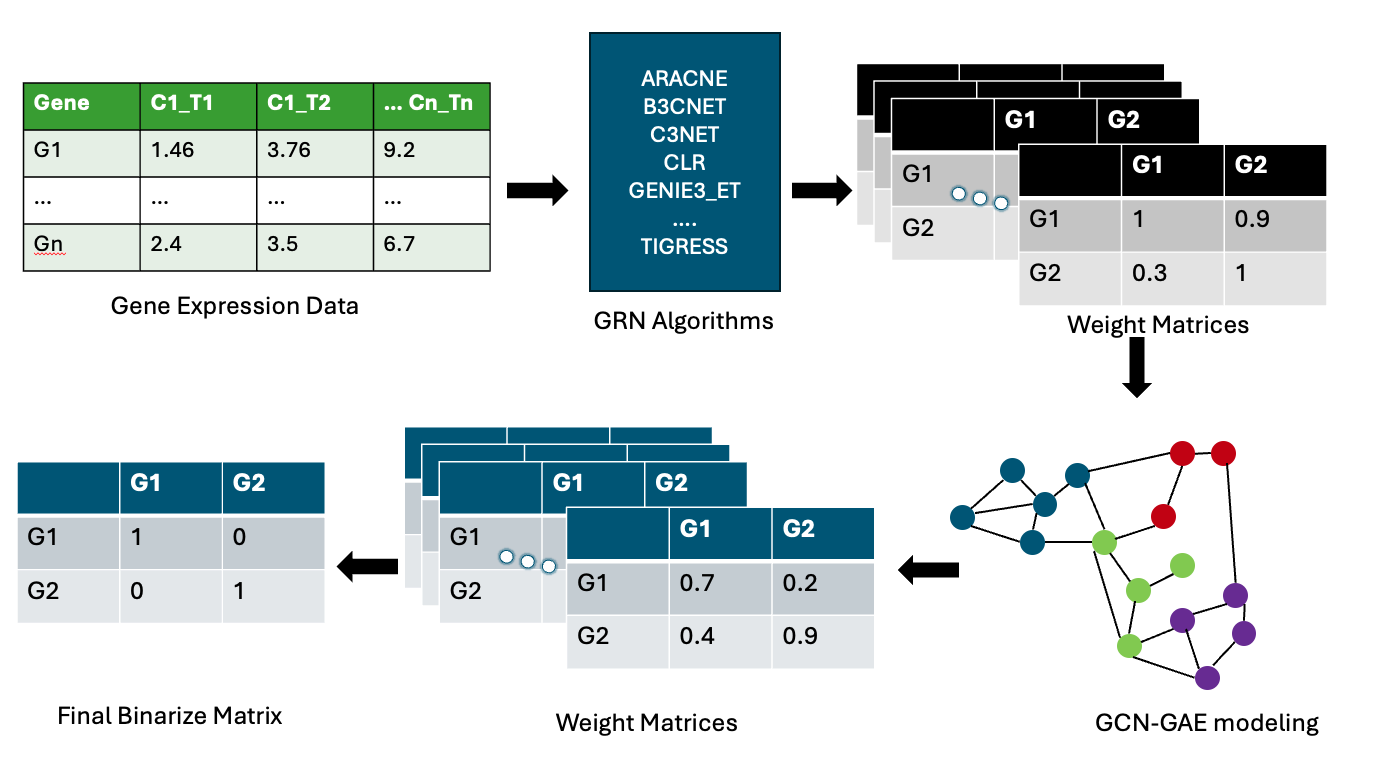
\includegraphics[width=0.8\linewidth]{fig/pipeline.png}
\caption{\label{fig:pipeline} Overview of the GCN workflow for constructing GRNs.}
\end{figure}


\subsection{EXPECTED OUTCOMES}
\subsubsection{Evaluation Metrics for the GCN Model}
Across the algorithms, the GCN-based GRNs generally exhibit superior AUROC scores compared to Raw GRNs (Figure~\ref{fig:evaluation_metrics_individual}, Figure~\ref{fig:evaluation_metrics}, Table~\ref{tab:performance_metrics_grouped}) for both individual and combined algorithms. This trend underscores the robustness of the GCN framework in distinguishing between true positive and false positive interactions. GCN excels in scenarios where generalization and structural integration are critical, highlighting its utility in broader applications.

\subsubsection*{Individual GRNs}
Raw GRNs tend to achieve higher AUPR scores (Figure~\ref{fig:aupr_individual}), particularly under conditions of high class imbalance where the number of true negatives outweighs true positives. This indicates the strength of Raw GRNs in pinpointing precise, high-confidence interactions without overgeneralization, aligning well with scenarios where precision is prioritized over recall. However, the GCN derived GRN consistently achieves higher AUROC values compared to the raw individual GRNs for most algorithms (Figure~\ref{fig:auroc_individual}). This suggests that integrating graph GCNs enhances the performance of GRN reconstructions by better capturing complex relationships in the data. The F1 score analysis (Figure~\ref{fig:f1score_individual}) demonstrates that GCN GRNs outperform Raw GRNs at lower filter thresholds (e.g., 0.2 to 0.5). However, as the thresholds increase (e.g., 0.7 and above), the F1 scores for both approaches converge or decline.

\textbf{GRN\_CLR, GRN\_GENIE3\_ET, and GRN\_GRNBOOST2} benefits the most from the GCN approach, particularly at lower thresholds. The integration of adjacency matrix information through GCN significantly enhances F1 scores (Figure~\ref{fig:f1score_individual}), demonstrating the potential of GCN to uncover meaningful gene interactions. While the GCN framework provides an edge over other raw GRNs, the performance gap is narrower for \textbf{GRN\_PCIT and GRN\_GRENIST} compared to other algorithms. This indicates modest improvements, suggesting that these algorithms might already capture significant structural information independently. \textbf{GRN\_TIGRESS} shows an advantage at lower thresholds, reflecting the ability to capture key interactions when more edges are included. However, as thresholds increase, the performance of both approaches converges, suggesting diminishing benefits from the GCN embeddings. \textbf{GRN\_LEAP and GRN\_NONLINEARODES} exhibit limited improvements or even  underperformance with the GCN approach. This suggests that the additional structure captured by GCN embeddings may not align well with the interaction patterns these algorithms inherently target. \textbf{GRN\_ARACNE and GRN\_BC3NET} display consistent improvements in F1 scores and AUROC, especially at intermediate thresholds. This highlights the balance GCN achieves between precision and recall, effectively leveraging latent structural information. \textbf{GRN\_MEOMI and GRN\_MRNETB} shows significant improvements in AUROC and moderate gains in AUPR. This suggests a broader generalization capability while retaining reasonable precision for these algorithms (Figure~\ref{fig:evaluation_metrics_individual}).

\begin{figure}[h!]
\centering
% Row 1: AUPR and AUROC side by side
\begin{subfigure}[b]{0.48\textwidth}
    \centering
    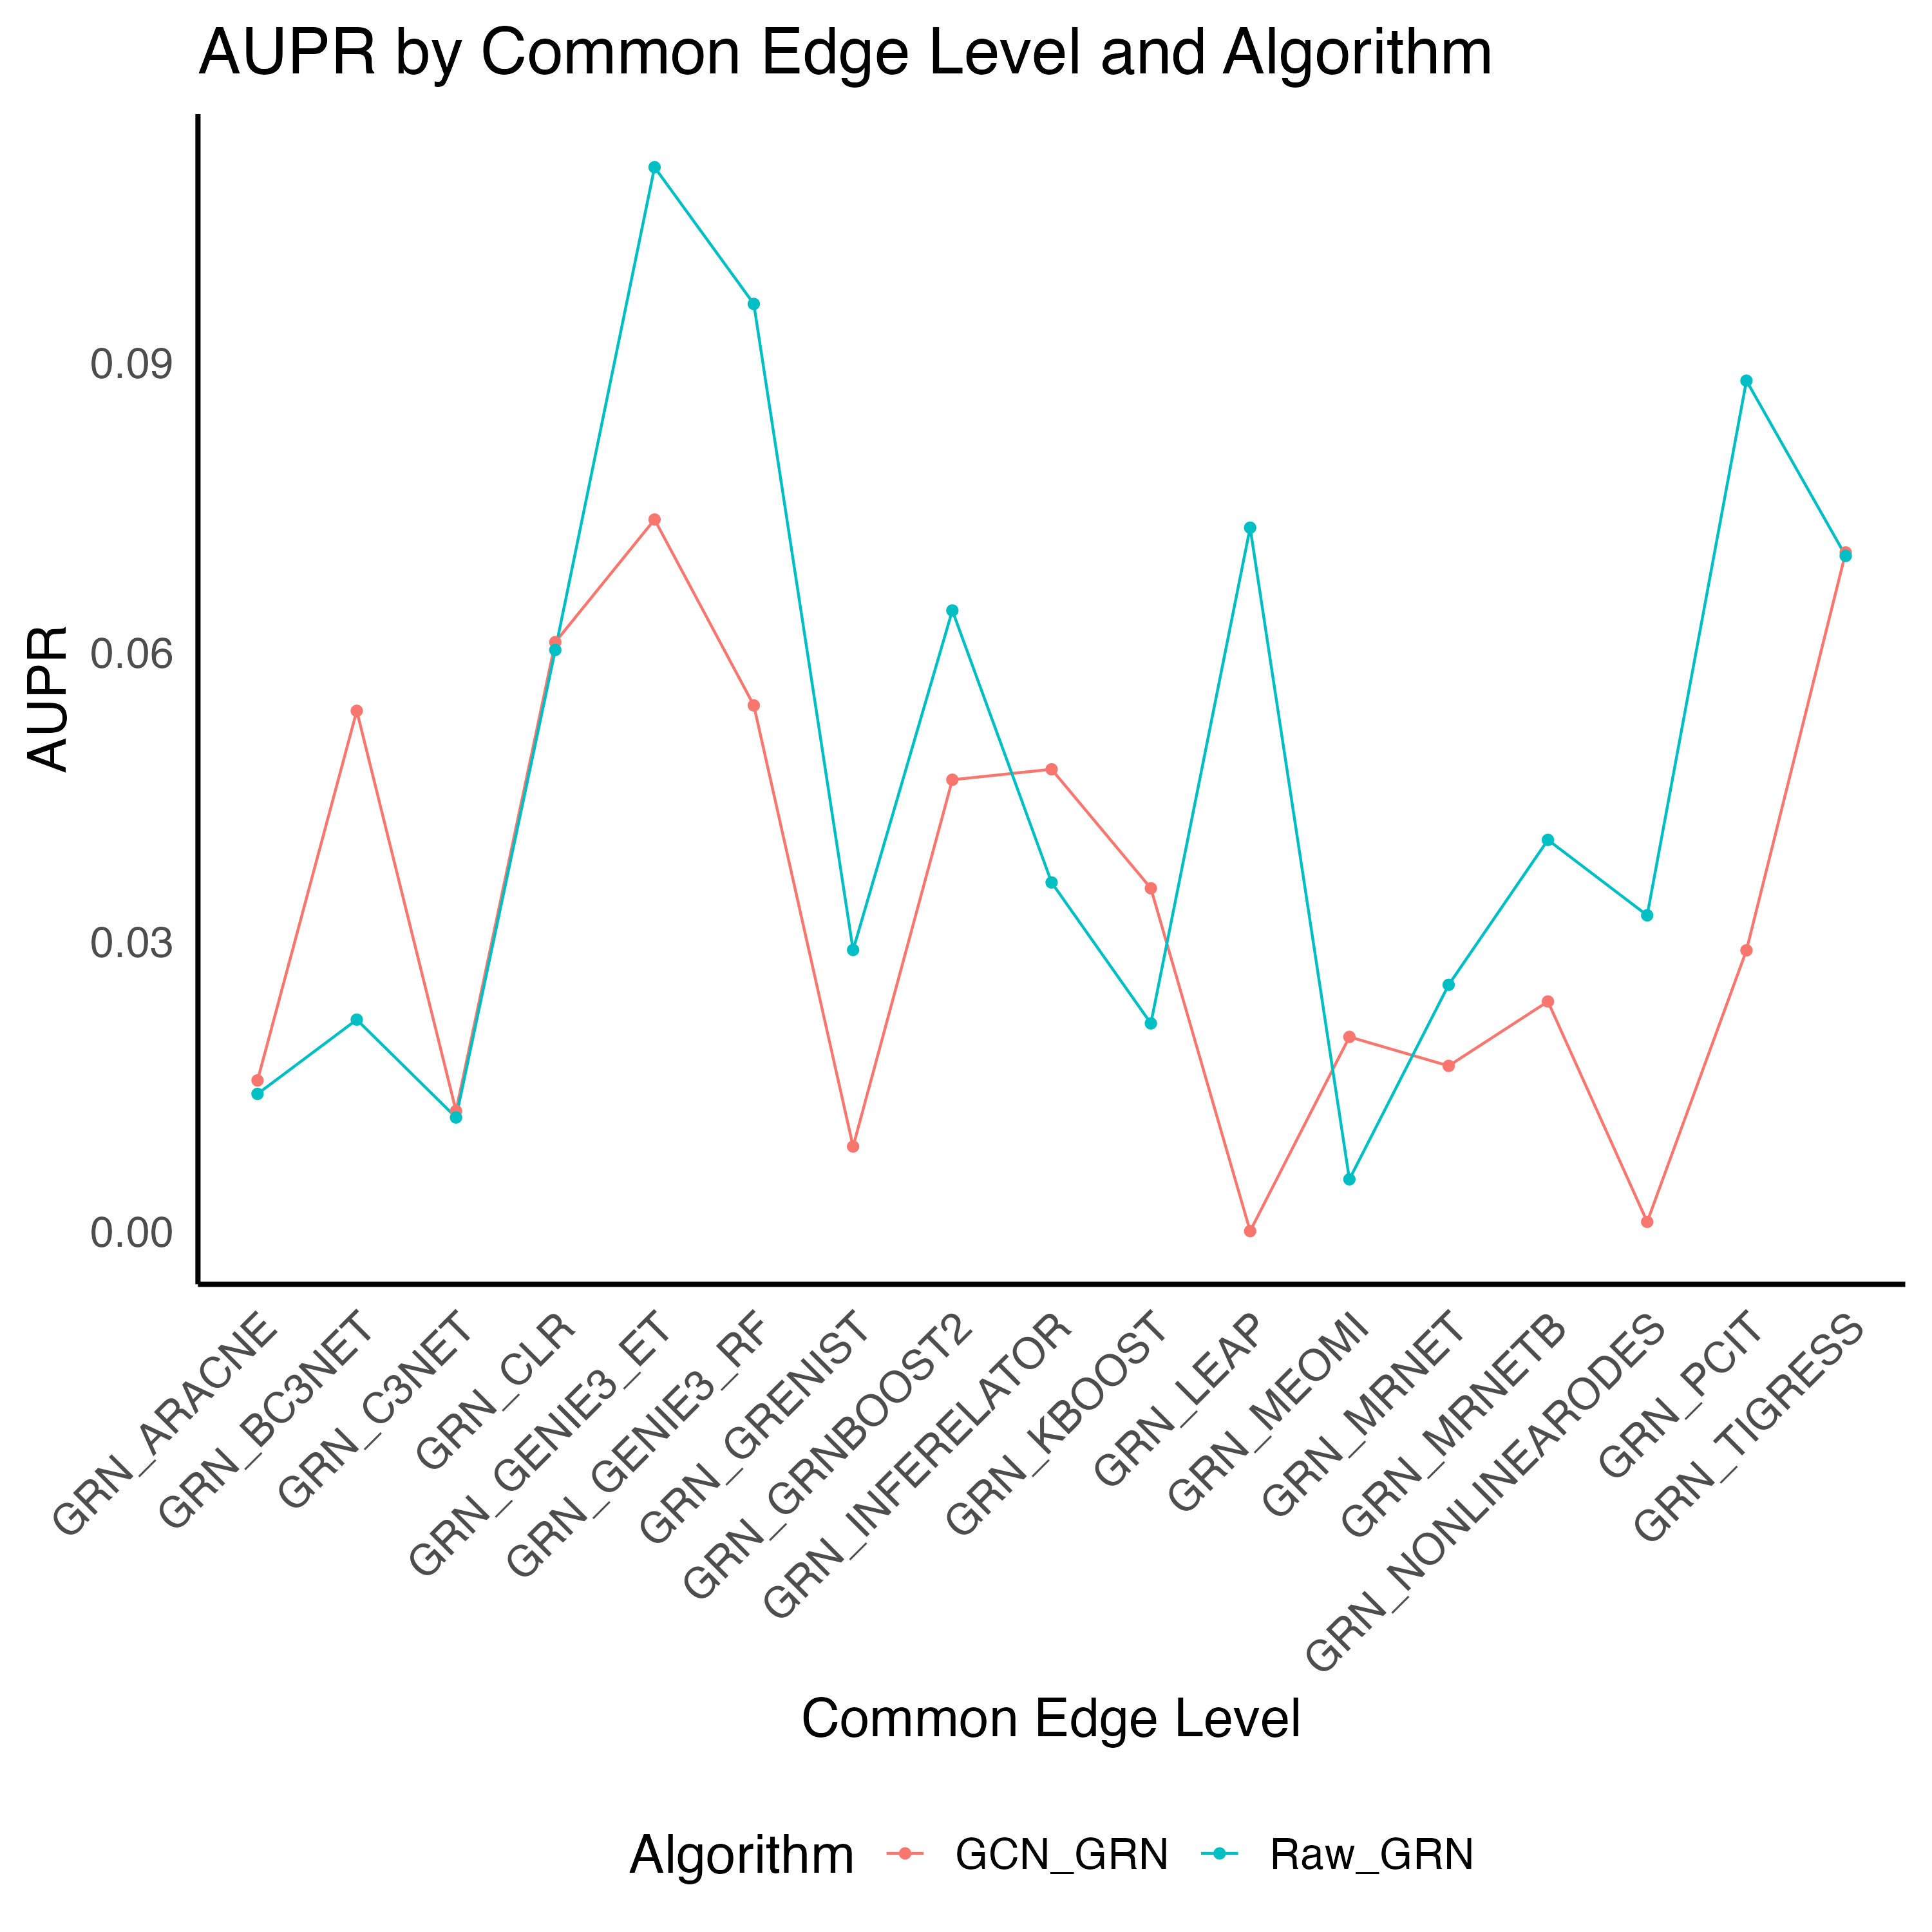
\includegraphics[width=\linewidth]{fig/AUPR_individual.png}
    \caption{AUPR}
    \label{fig:aupr_individual}
\end{subfigure}
\hfill
\begin{subfigure}[b]{0.48\textwidth}
    \centering
    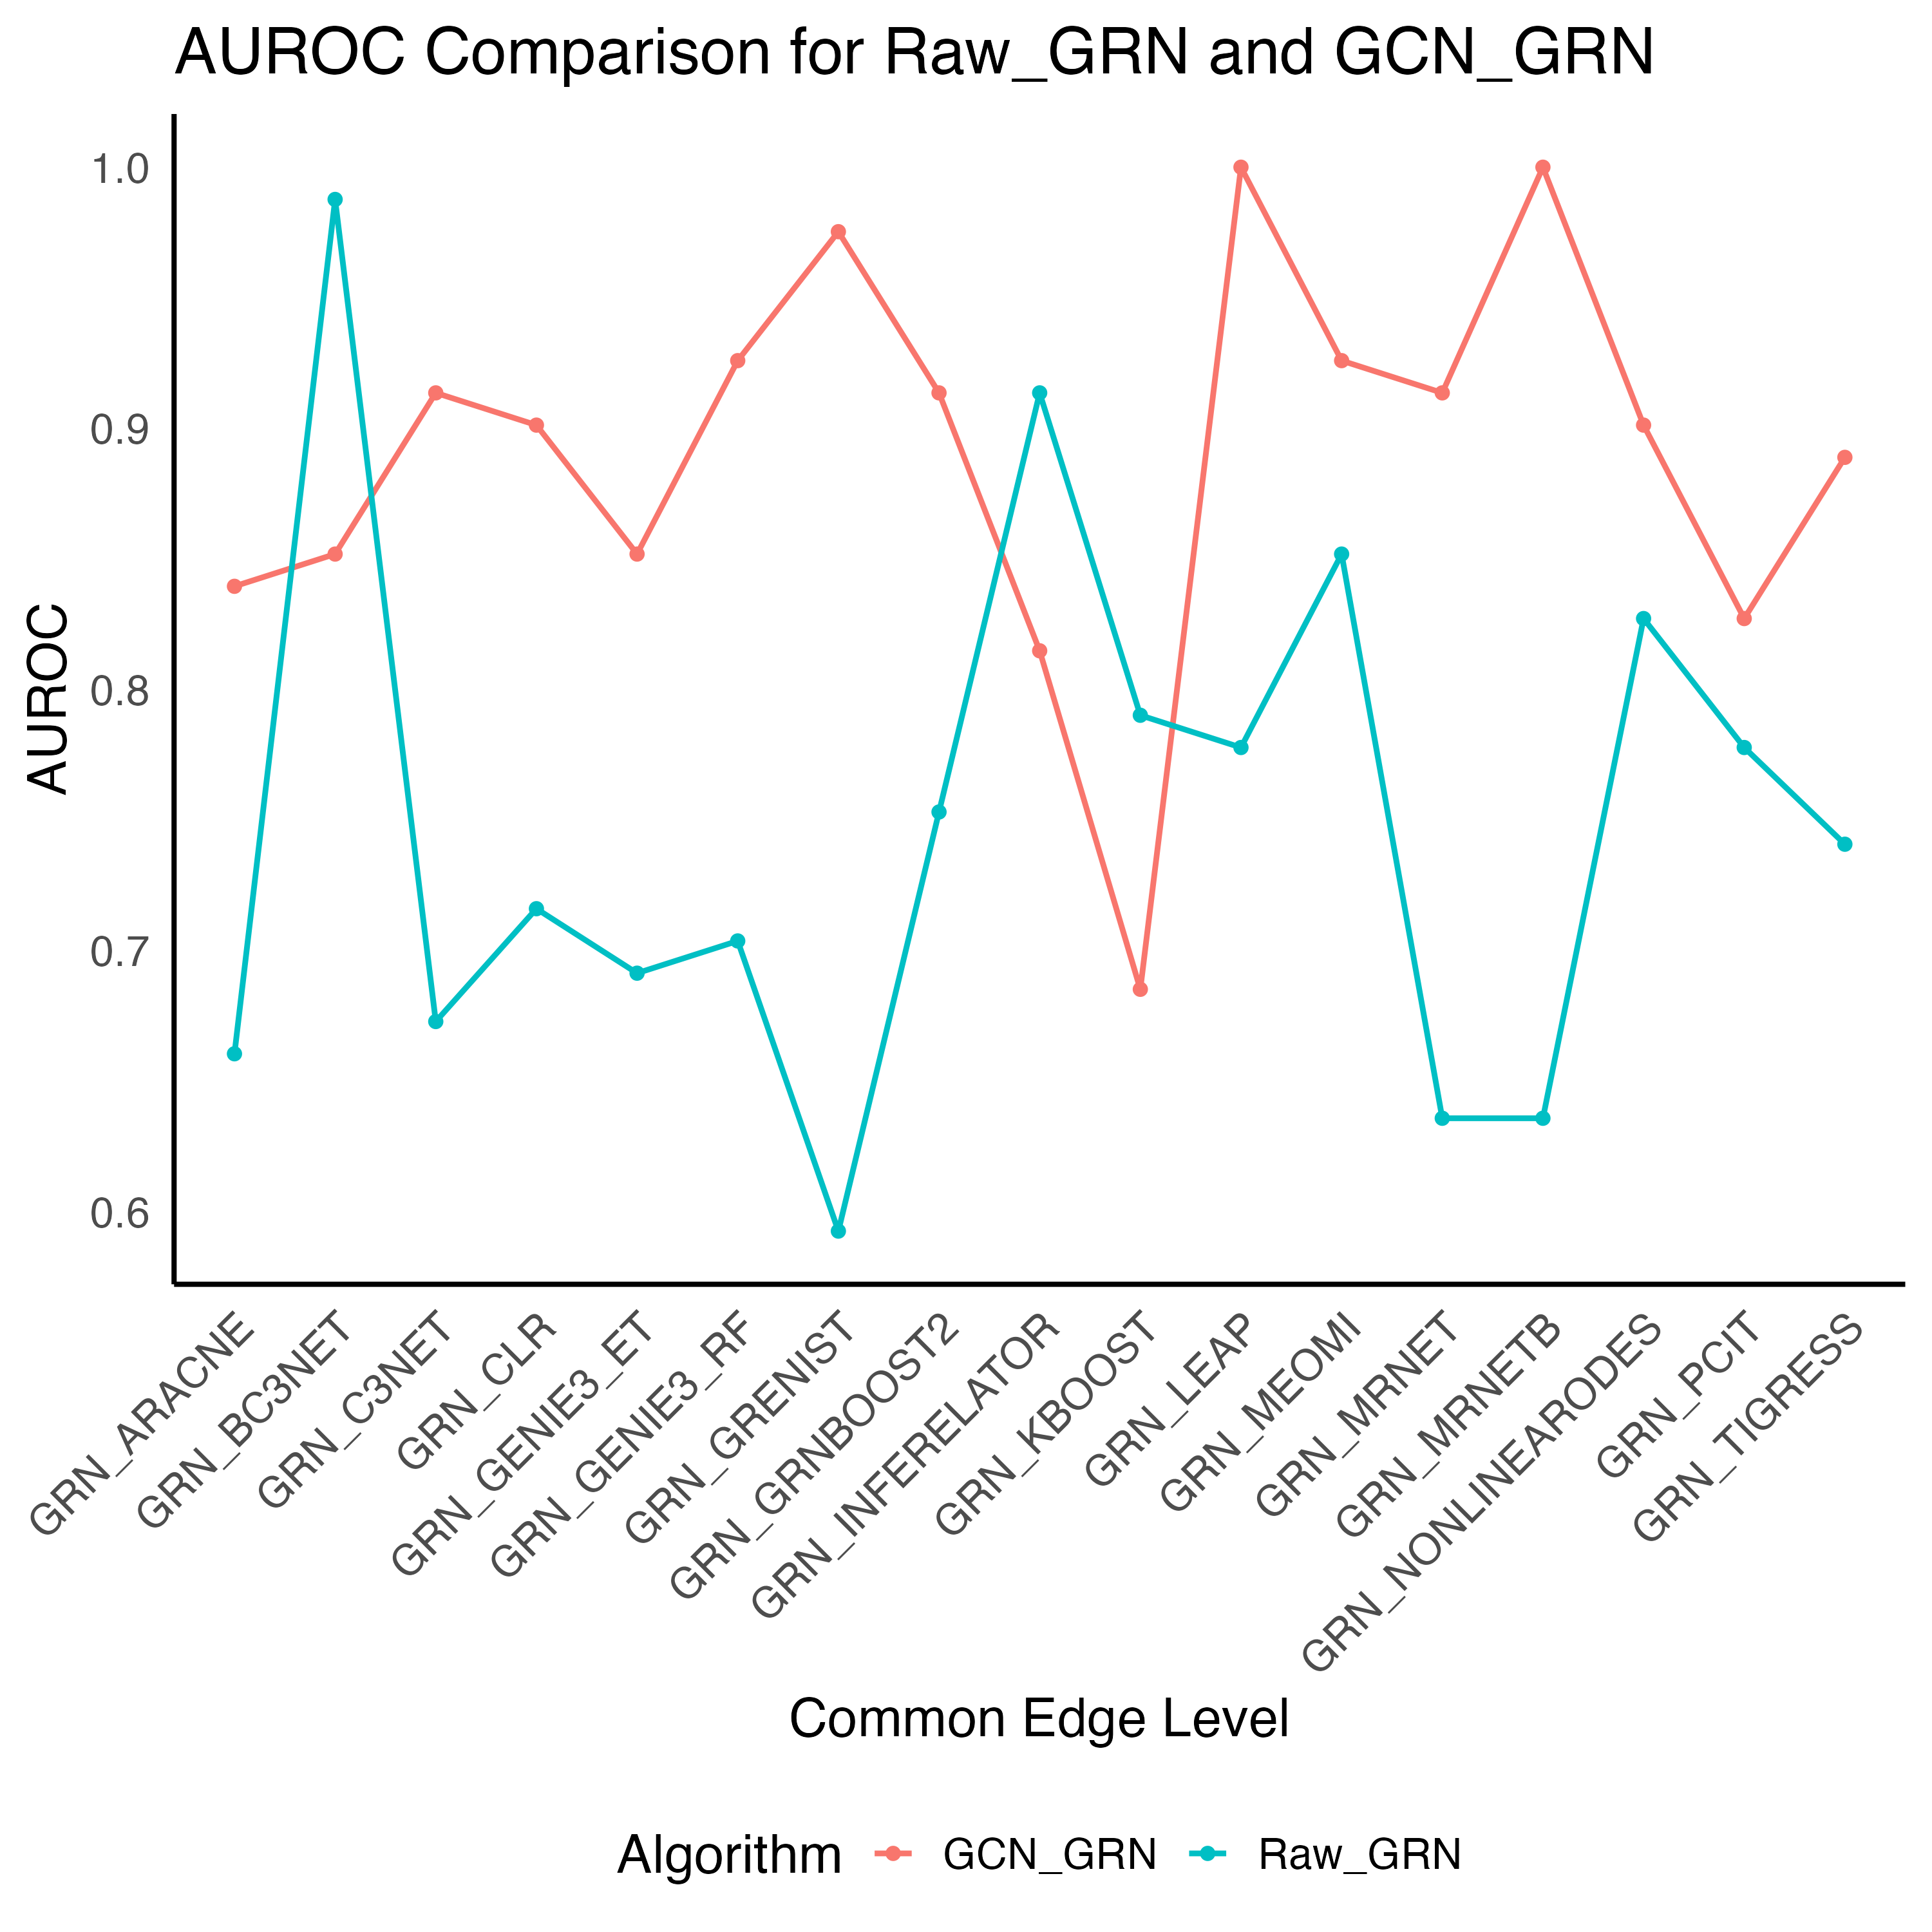
\includegraphics[width=\linewidth]{fig/AUROC_individual.png}
    \caption{AUROC}
    \label{fig:auroc_individual}
\end{subfigure}

\vspace{1em} % Space between rows

% Row 2: F1-Score
\begin{subfigure}[b]{0.9\textwidth}
    \centering
    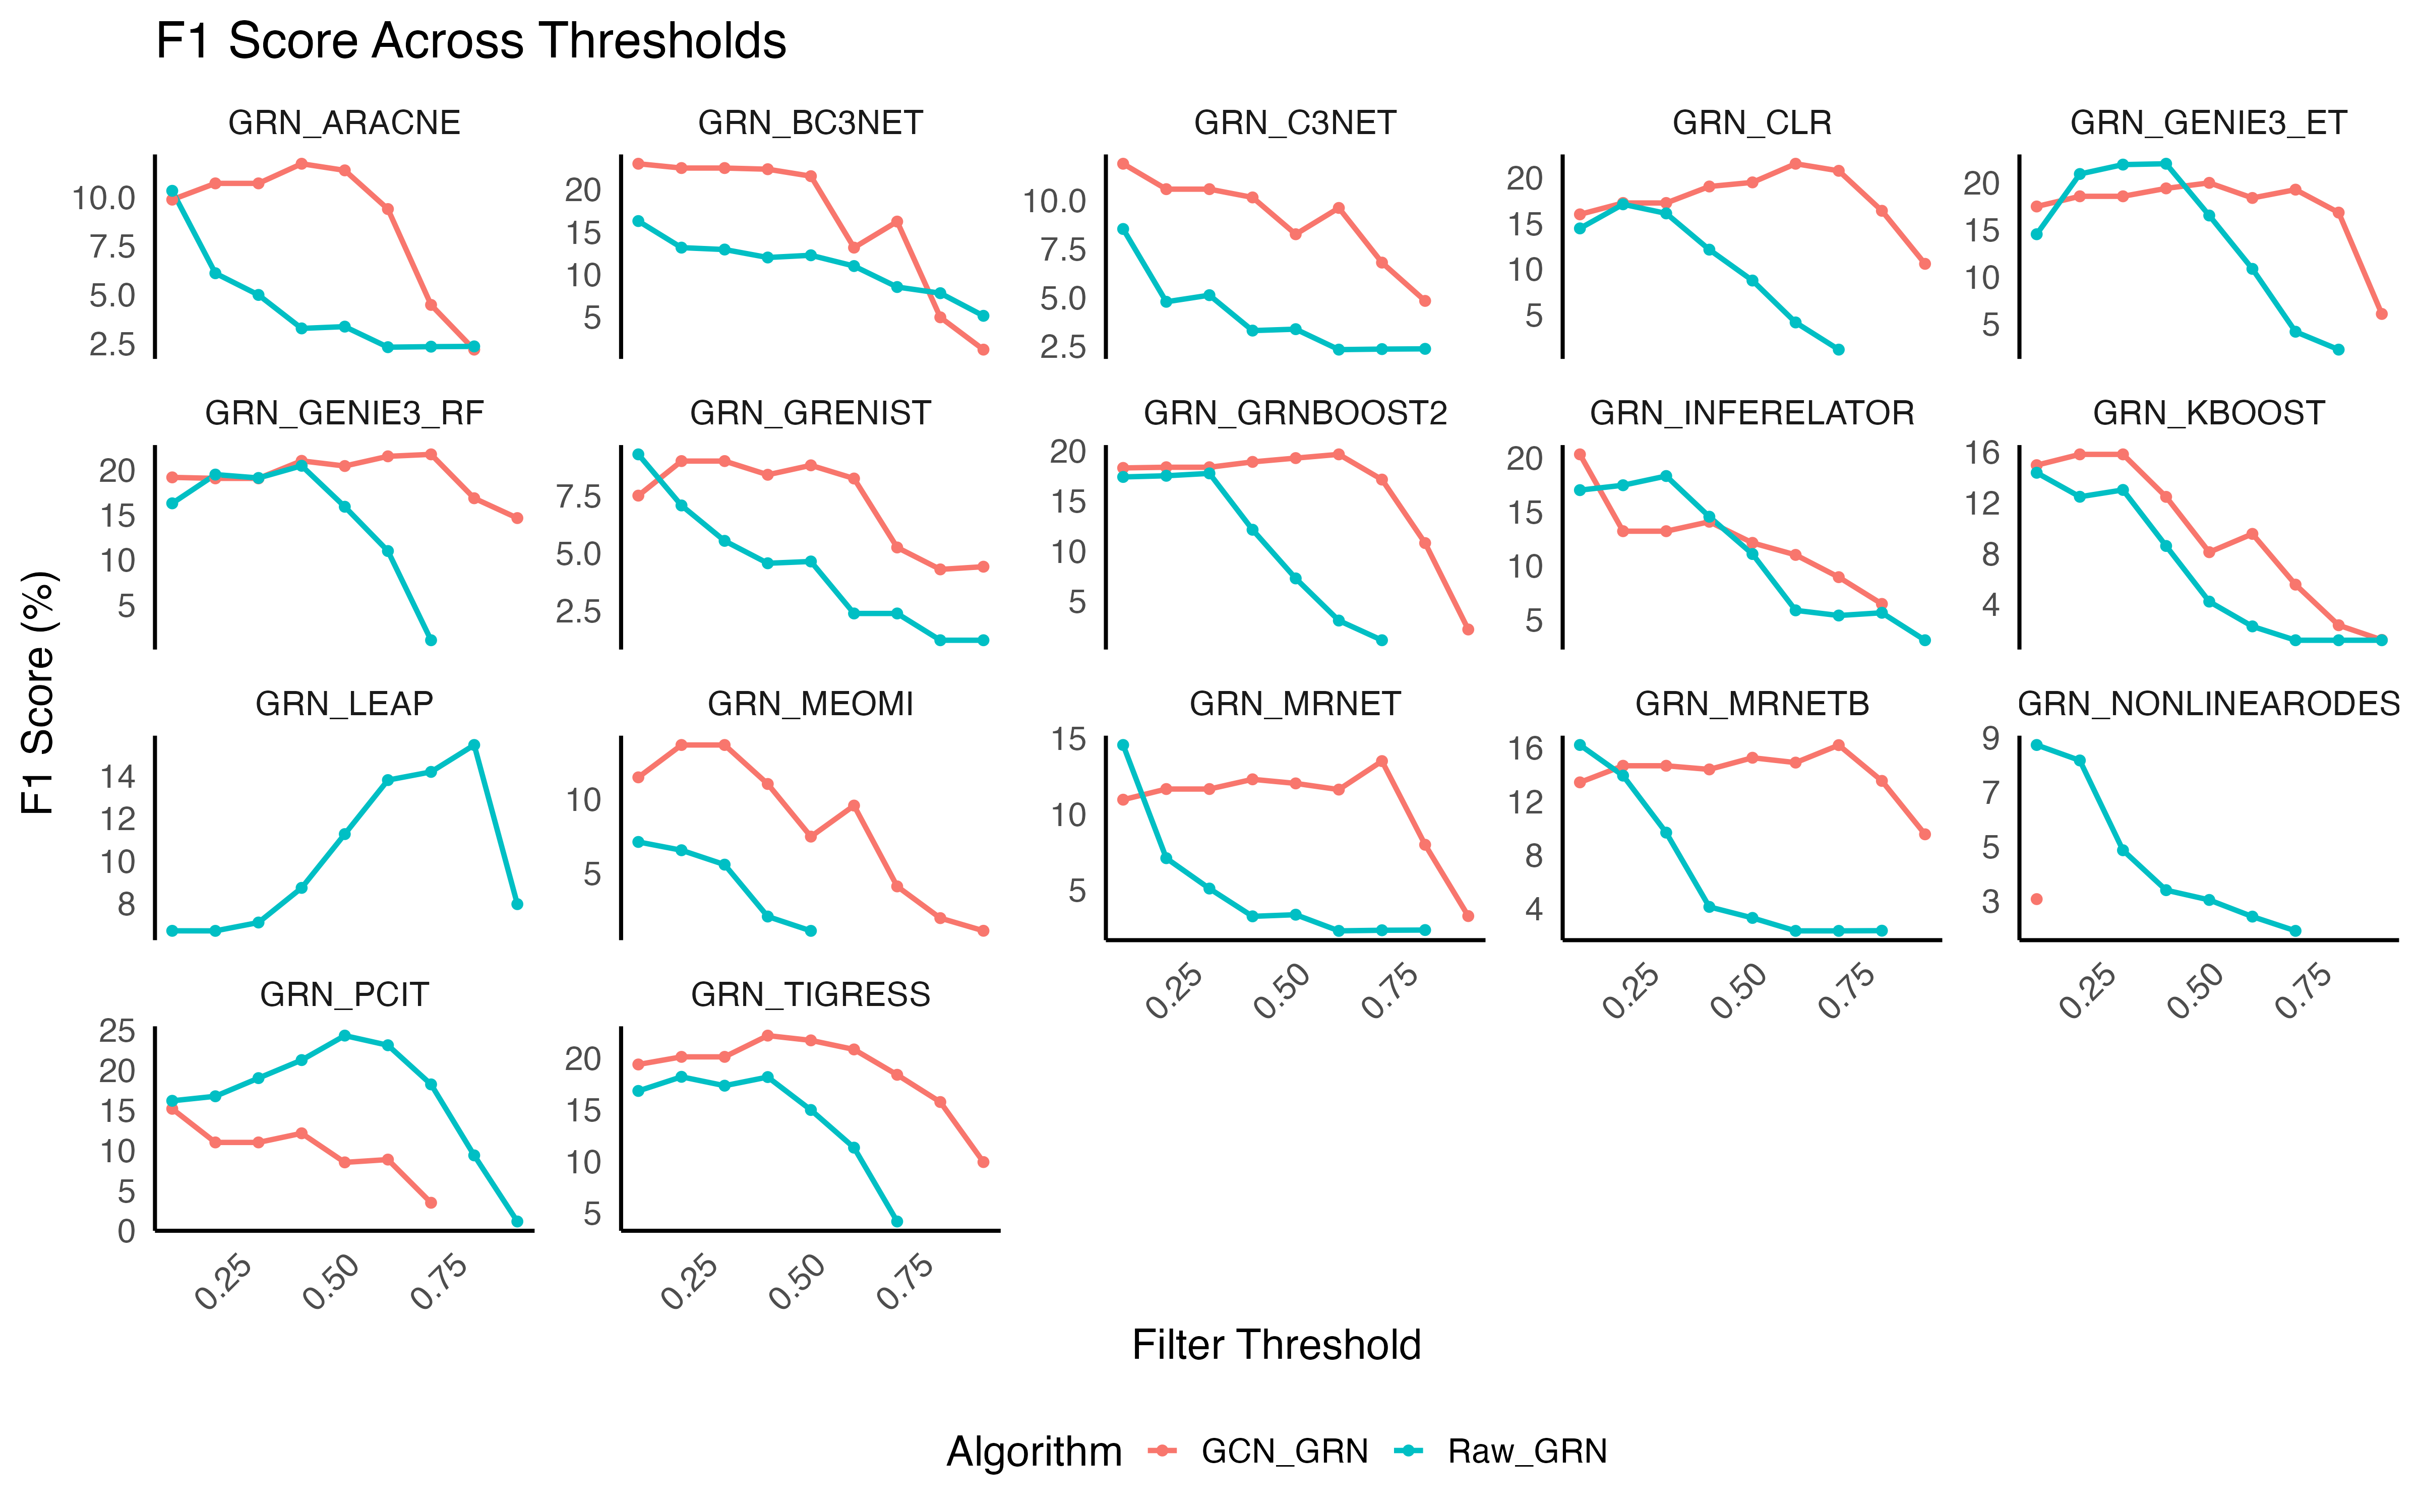
\includegraphics[width=\linewidth]{fig/F1_Score_individual.png}
    \caption{F1-Score}
    \label{fig:f1score_individual}
\end{subfigure}

\caption{Performance evaluation metrics for the reconstructed individual GRNs for raw and GCN-derived GRN using the DREAM4 dataset. (a) AUPR, (b) AUROC, and (c) F1-Score.}
\label{fig:evaluation_metrics_individual}
\end{figure}


\subsubsection*{Combined GRNs}
We aggregated predictions from multiple algorithms into a comprehensive adjacency matrix for raw the GCN-derived model (Table~\ref{tab:performance_metrics_grouped}). \textit{Raw\_GRN} denotes the aggregation between individual GRNs, and \textit{GCN\_GRN} denotes the aggregation between GCN-derived GRNs. This GCN integration not only retained key gene interactions identified by the individual algorithms but also revealed novel interactions that were not captured by the raw GRNs of the individual methods. These new interactions may stem from the model's ability to leverage the latent space representations of genes. This capability could represent a significant step forward in network inference, offering new insights into gene interactions that were previously overlooked. 

Fig.~\ref{fig:evaluation_metrics} compares the performance of reconstructed Gene GRNs, focusing on GCN-derived GRNs (\textit{GCN\_GRN}) and Raw GRNs (\textit{Raw\_GRN}) across three metrics: AUPR, AUROC, and F1-Score. Panel (a) shows the Area Under the Precision-Recall Curve (AUPR) across different levels of common edges. \textit{GCN\_GRN} consistently outperforms \textit{Raw\_GRN} at all thresholds, with peak performance observed for edges shared across a moderate number of algorithms (e.g., Combined\_edges~$>$3). This highlights \textit{GCN\_GRN}'s ability to identify high-confidence interactions while capturing biologically meaningful patterns missed by individual GRNs. Panel (b) compares the Area Under the Receiver Operating Characteristic Curve (AUROC), revealing that \textit{GCN\_GRN} maintains superior performance across all edge thresholds. Notably, the performance gap between \textit{GCN\_GRN} and \textit{Raw\_GRN} widens at stricter thresholds, demonstrating the robustness of the GCN model in prioritizing true positives while minimizing false positives. Panel (c) evaluates the F1-Score across varying filter thresholds and common edge levels. \textit{GCN\_GRN} consistently achieves higher F1-Scores compared to \textit{Raw\_GRN}, with the advantage being most prominent at lower thresholds. As filter thresholds increase, F1-Scores decline for both approaches, reflecting the trade-off between precision and recall when stricter criteria are applied. Collectively, these results demonstrate that the \textit{GCN\_GRN} method not only integrates the strengths of multiple GRN algorithms but also uncovers novel and biologically significant interactions, offering a more accurate and comprehensive representation of gene regulatory mechanisms.

\begin{table}[h!]
\centering
\caption{Performance Metrics for Algorithms}
\begin{tabular}{@{}lcccc@{}}
\toprule
\textbf{Algorithm} & \multicolumn{2}{c}{\textbf{Raw}} & \multicolumn{2}{c}{\textbf{GCN}} \\ \cmidrule(lr){2-3} \cmidrule(lr){4-5}
                   & \textbf{AUPR} & \textbf{AUROC}   & \textbf{AUPR} & \textbf{AUROC}   \\ \midrule
ARACNE        & 0.0142        & 0.6605           & 0.0156        & 0.8395           \\
BC3NET        & 0.0219        & 0.9877           & 0.0539        & 0.8519           \\
C3NET         & 0.0118        & 0.6728           & 0.0125        & 0.9136           \\
CLR           & 0.0602        & 0.7160           & 0.0610        & 0.9012           \\
GENIE3\_ET    & 0.1103        & 0.6914           & 0.0737        & 0.8519           \\
GENIE3\_RF    & 0.0961        & 0.7037           & 0.0545        & 0.9259           \\
GRENIST       & 0.0291        & 0.7531           & 0.0088        & 0.9753           \\
GRNBOOST2     & 0.0643        & 0.9136           & 0.0468        & 0.9136           \\
INFERELATOR   & 0.0361        & 0.7901           & 0.0479        & 0.8148           \\
KBOOST        & 0.0215        & 0.7778           & 0.0355        & 0.6852           \\
LEAP          & 0.0729        & 0.8519           & 0             & 1                \\
MEOMI         & 0.0054        & 0.6358           & 0.0201        & 0.9259           \\
MRNET         & 0.0255        & 0.6358           & 0.0171        & 0.9136           \\
MRNETB        & 0.0405        & 0.8272           & 0.0238        & 1                \\
NONLINEARODES & 0.0327        & 0.7778           & 0.0010        & 0.9012           \\
PCIT          & 0.0881        & 0.7407           & 0.0291        & 0.8272           \\
TIGRESS       & 0.0700        & 0.5926           & 0.0703        & 0.8889           \\
Combined\_edges\geq$1 & 0.0723        & 0.7654           & 0.0574        & 0.9136           \\
Combined\_edges\geq$2 & 0.1129        & 0.7407           & 0.0760        & 0.9136           \\
Combined\_edges\geq$3 & 0.1044        & 0.7160           & 0.0798        & 0.9012           \\
Combined\_edges\geq$4 & 0.0966        & 0.7284           & 0.0824        & 0.8765           \\
Combined\_edges\geq$5 & 0.0912        & 0.7160           & 0.0802        & 0.8642           \\
Combined\_edges\geq$6 & 0.0794        & 0.7160           & 0.0777        & 0.8395           \\
Combined\_edges\geq$7 & 0.0687        & 0.7284           & 0.0753        & 0.8025           \\
Combined\_edges\geq$8 & 0.0540        & 0.6914           & 0.0629        & 0.7901           \\
Combined\_edges\geq$9 & NaN           & 0.6790           & 0.0452        & 0.7901           \\ \bottomrule
\end{tabular}
\label{tab:performance_metrics_grouped}
\end{table}

\begin{figure}[h!]
\centering
% Row 1: AUPR and AUROC side by side
\begin{subfigure}[b]{0.48\textwidth}
    \centering
    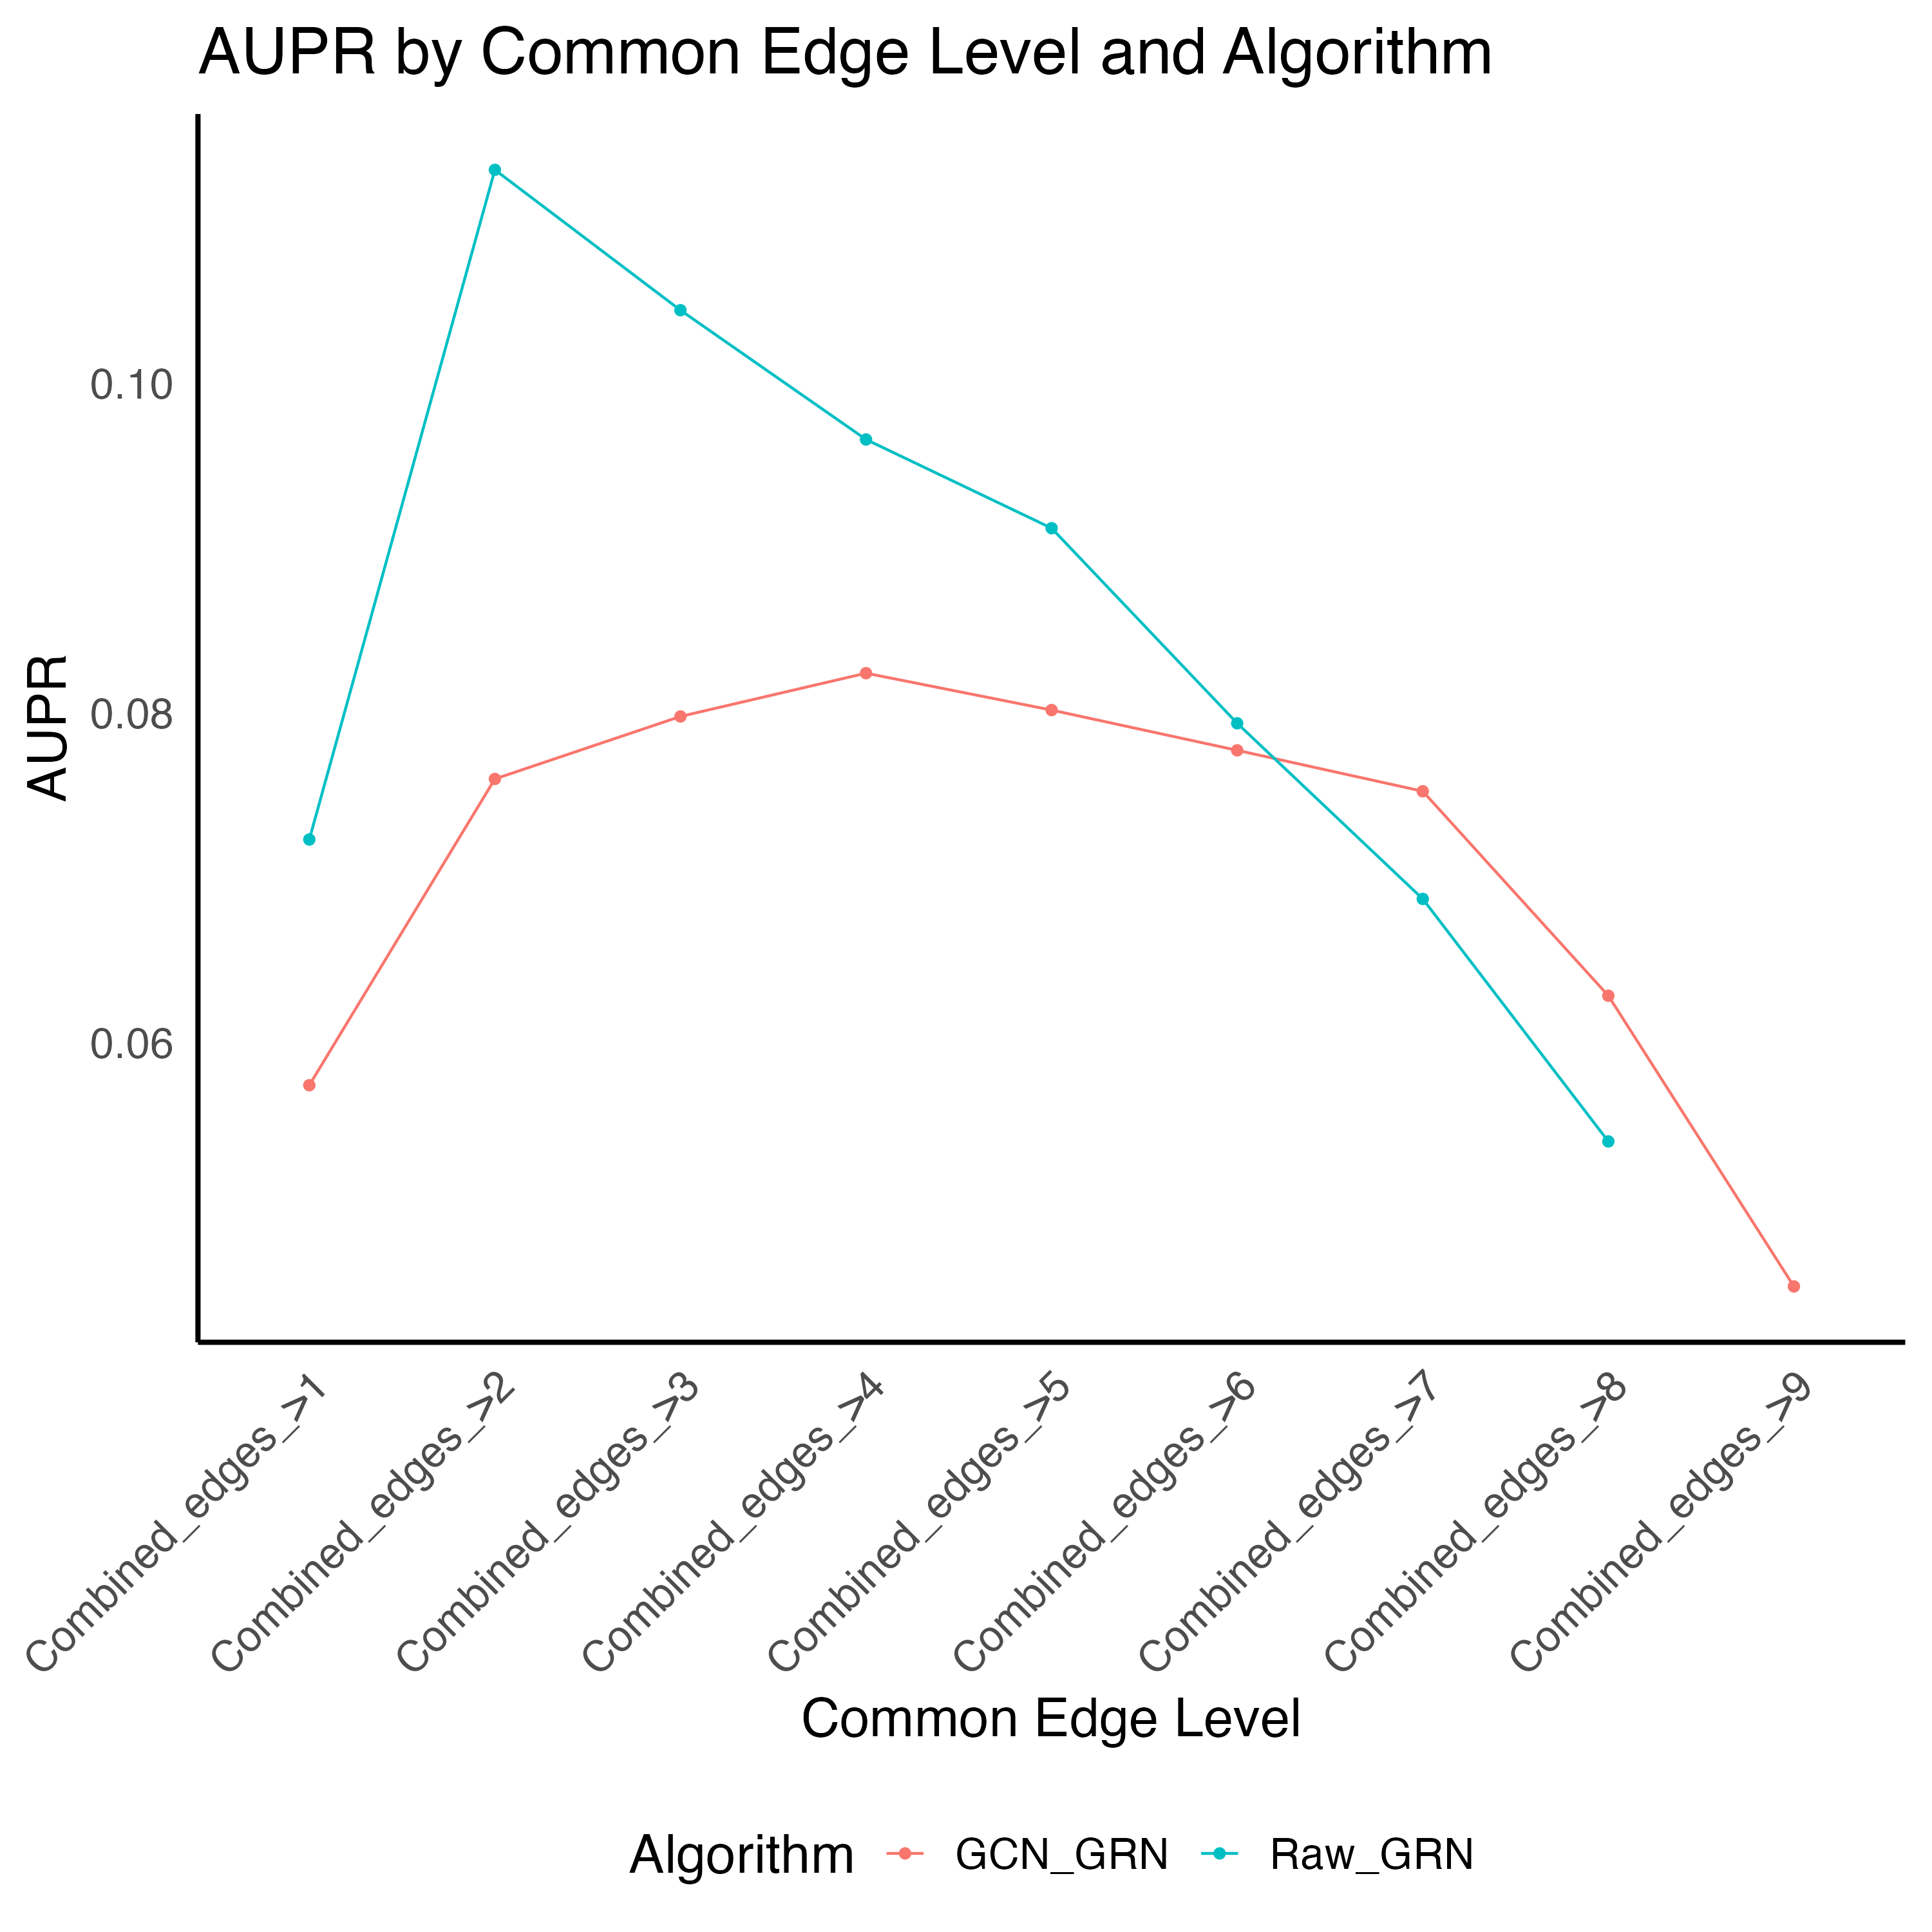
\includegraphics[width=\linewidth]{fig/AUPR.png}
    \caption{AUPR}
    \label{fig:aupr}
\end{subfigure}
\hfill
\begin{subfigure}[b]{0.48\textwidth}
    \centering
    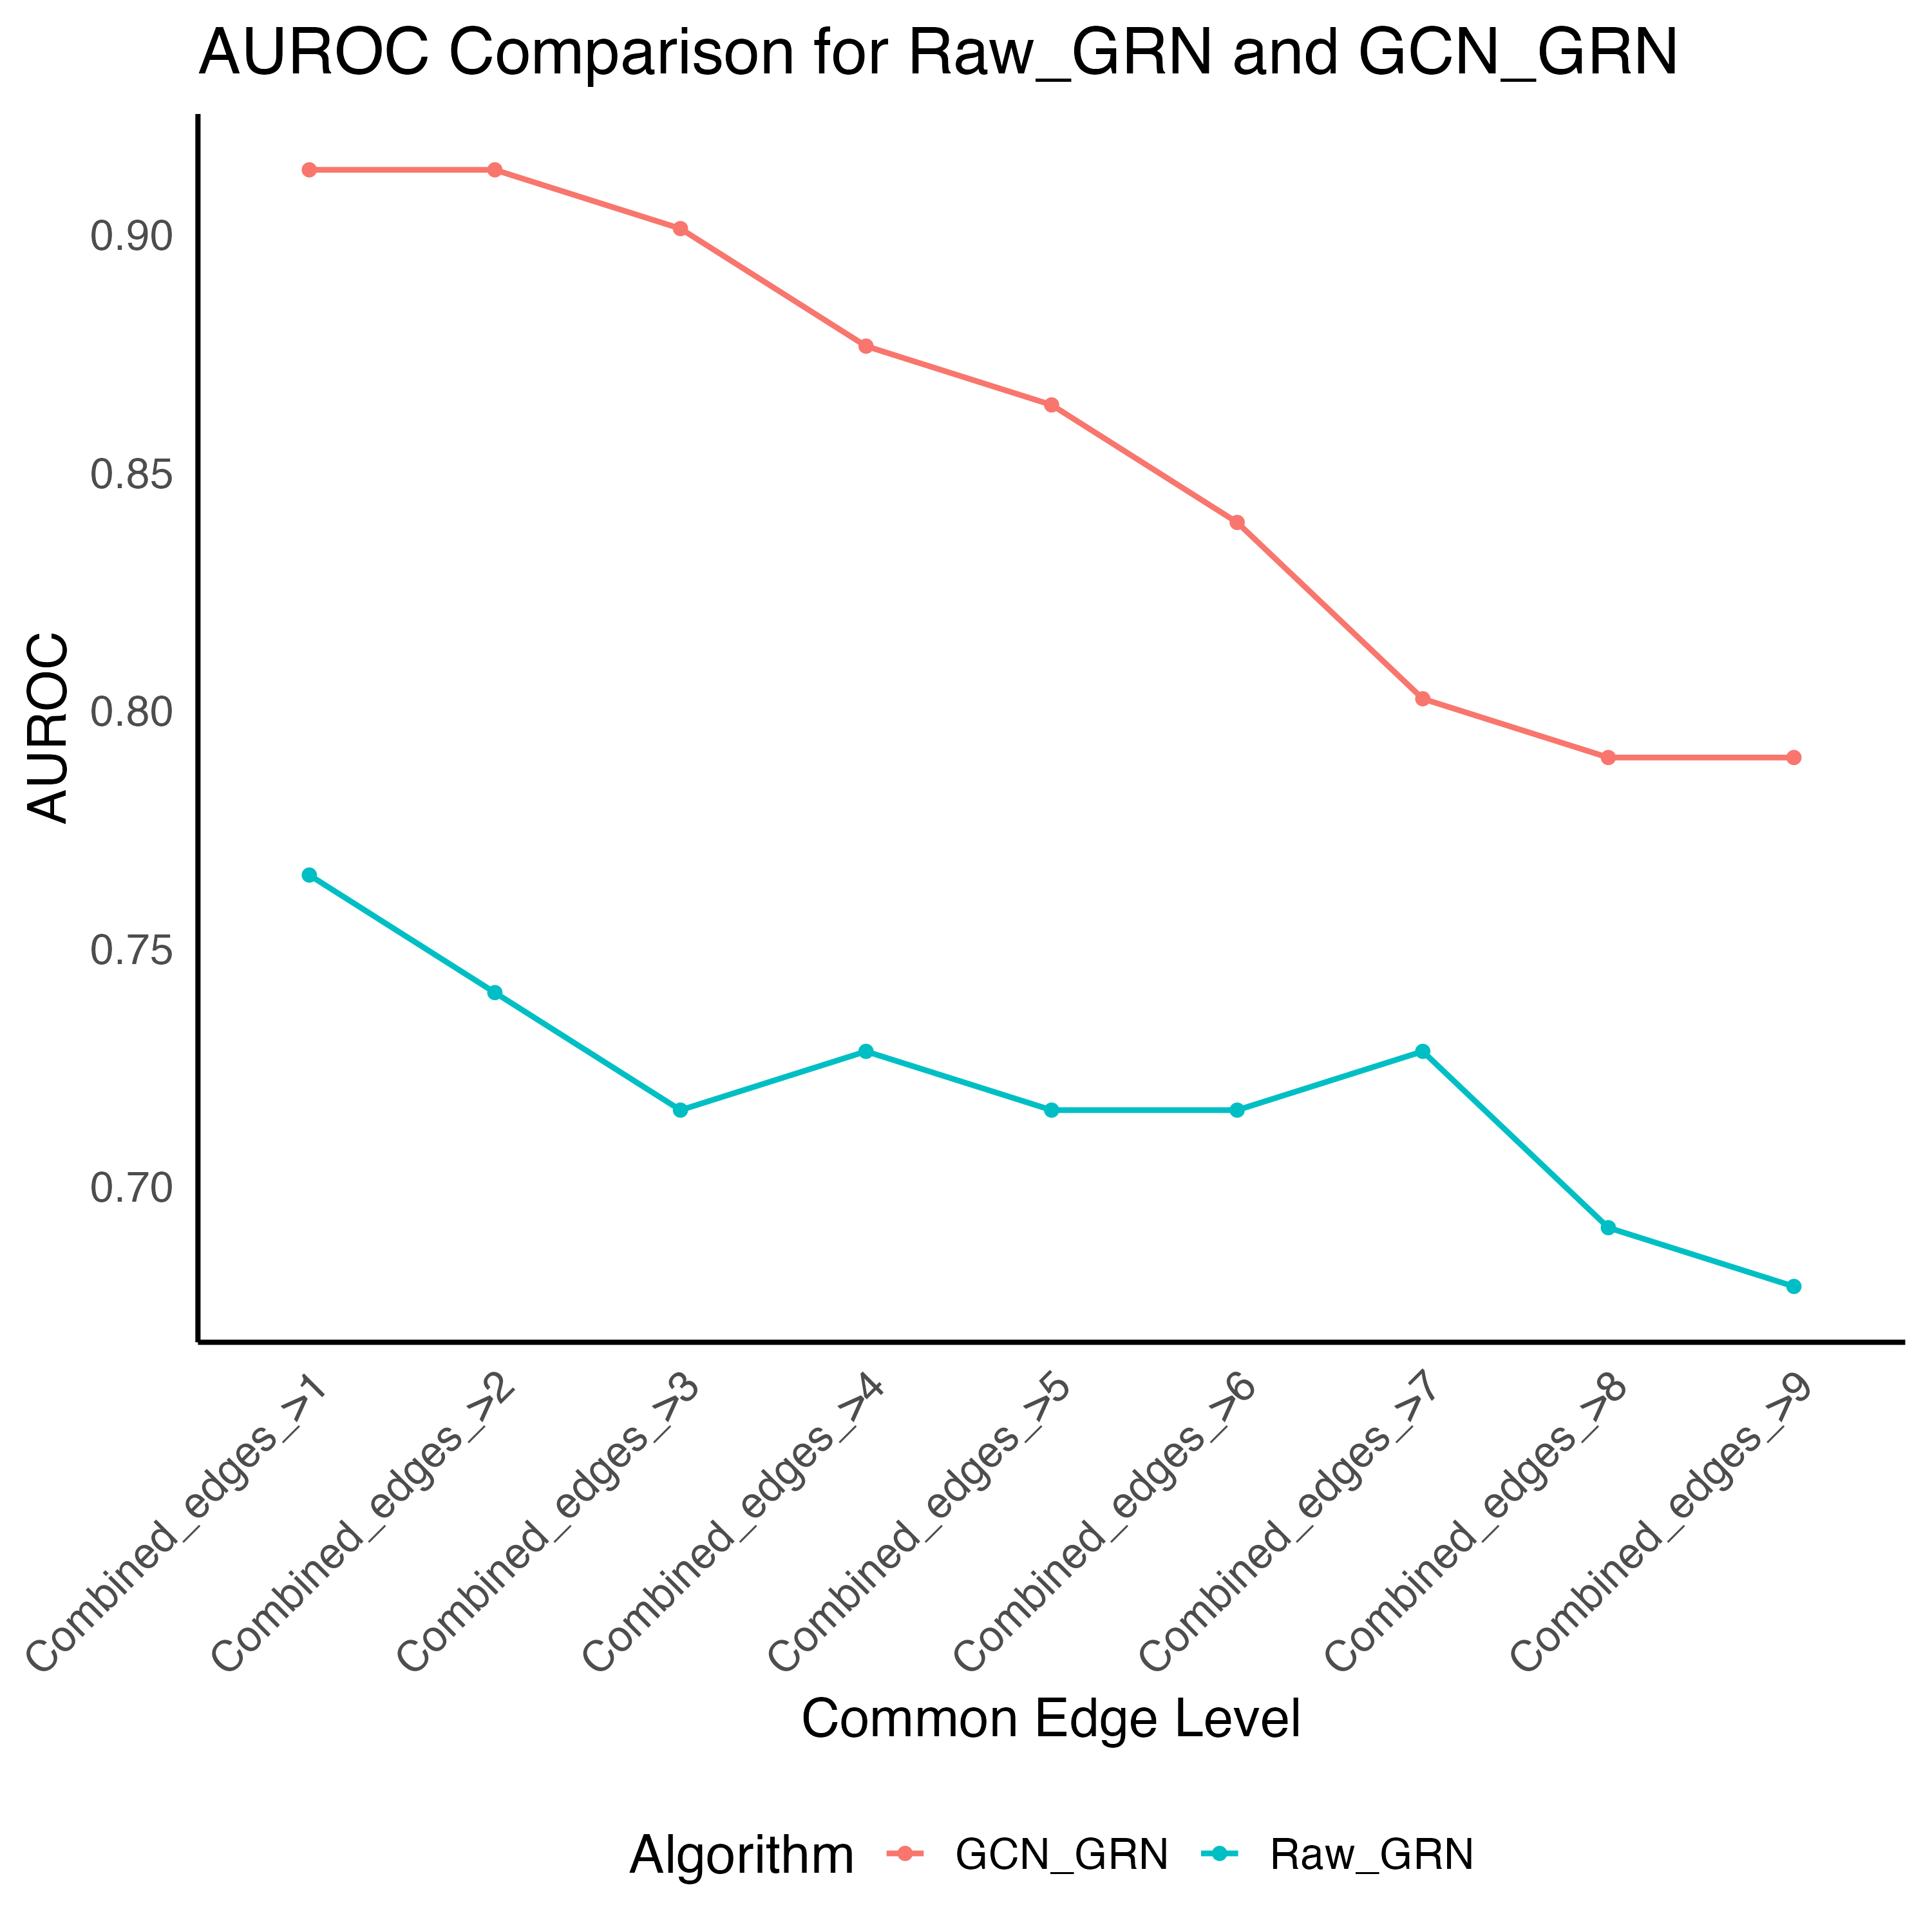
\includegraphics[width=\linewidth]{fig/AUROC.png}
    \caption{AUROC}
    \label{fig:auroc}
\end{subfigure}

\vspace{1em} % Space between rows

% Row 2: F1-Score
\begin{subfigure}[b]{0.78\textwidth}
    \centering
    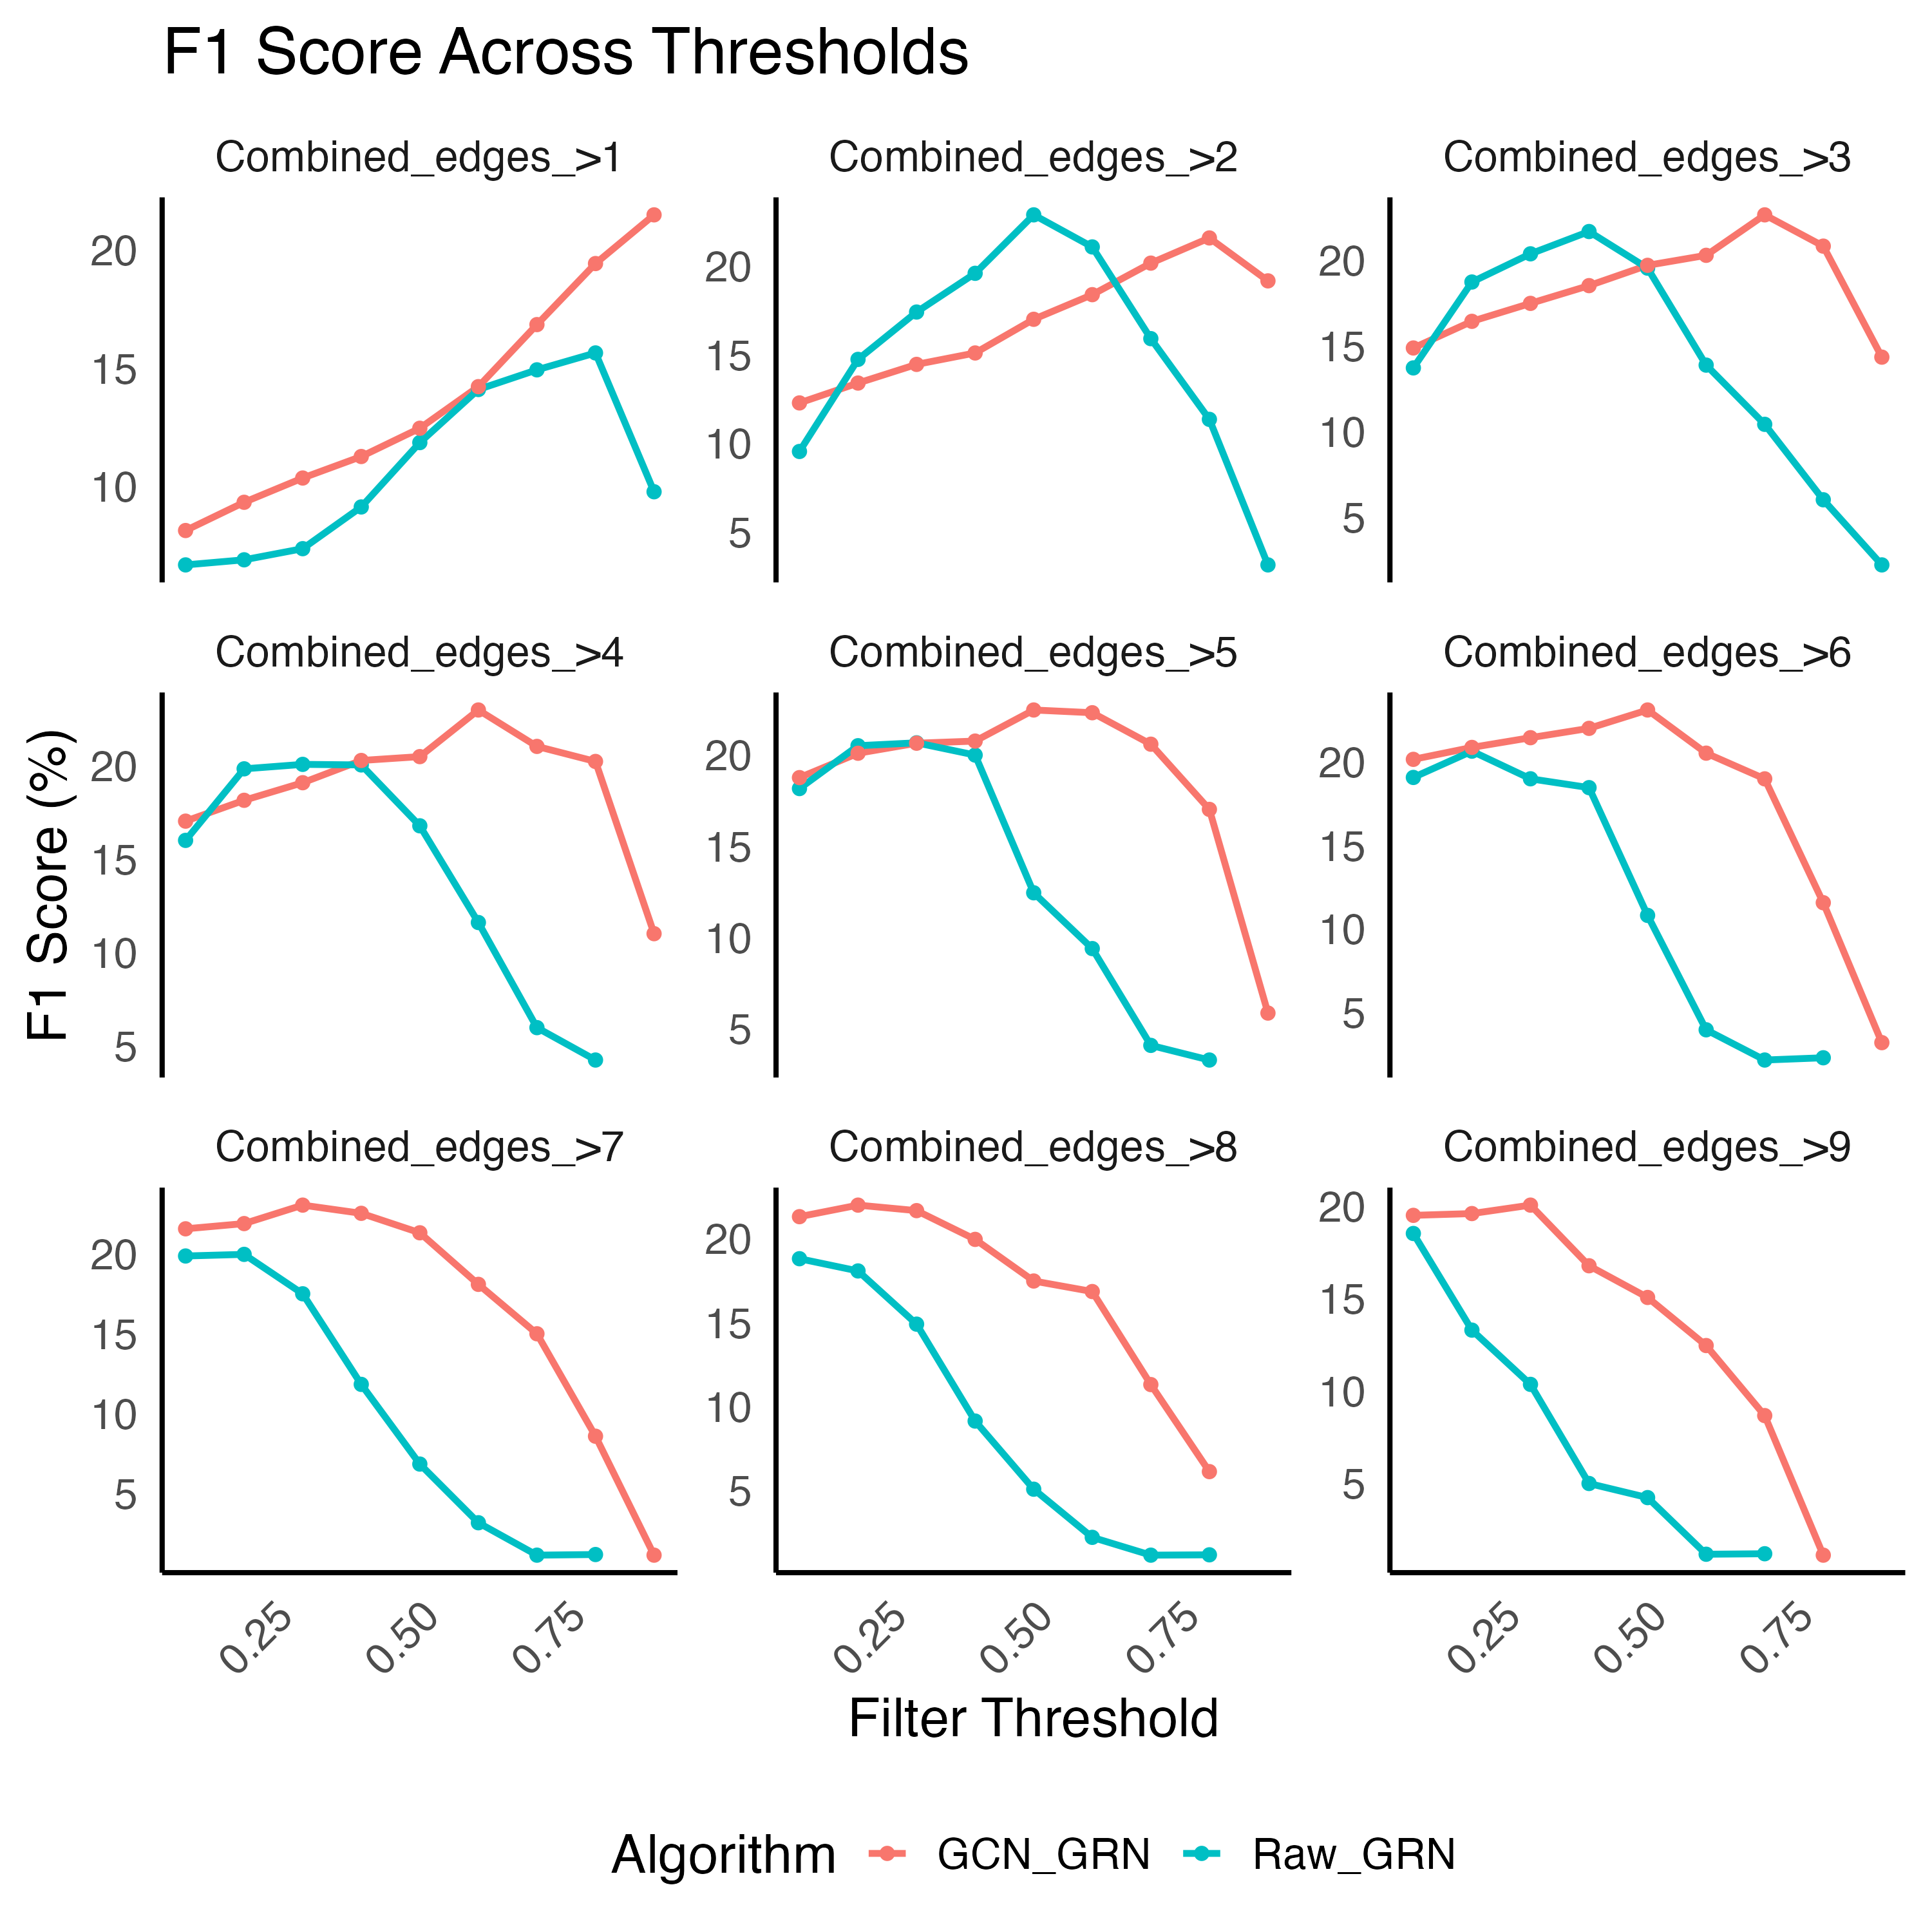
\includegraphics[width=\linewidth]{fig/F1_Score.png}
    \caption{F1-Score}
    \label{fig:f1score}
\end{subfigure}

\caption{Performance evaluation metrics for the reconstructed combined GRNs for raw and GCN derived GRN using the DREAM4 dataset. (a) AUPR, (b) AUROC, and (c) F1-Score.}
\label{fig:evaluation_metrics}
\end{figure}


\subsubsection{T-SNE Analysis for the GCN-Derived GRNs}
The t-SNE analysis was conducted to visualize the latent embeddings generated by the GCN model applied to adjacency matrices derived from 17 different GRN inference algorithms (Fig.~\ref{fig:tsne_embeddings}). These embeddings were extracted after training the GCN on the adjacency matrices, and they represent the relationships between genes in a reduced-dimensional latent space. Each dot in the t-SNE plots corresponding to a gene.

The resulting t-SNE plots, displayed for each GRN inference algorithm, revealed distinct patterns in the latent space. In some algorithms, such as \texttt{`GRN\_PCIT`} and \texttt{`GRN\_CLR`}, the embeddings formed well-defined clusters, indicating that the adjacency matrices generated by these algorithms contained meaningful relationships that the GCN successfully captured. These clusters likely represent groups of genes that are co-regulated, share functional similarities, or participate in related biological pathways. In contrast, other algorithms, such as \texttt{`GRN\_LEAP`} and \texttt{`GRN\_NONLINEARODES`}, displayed sparse or poorly grouped points, which may suggest noisier adjacency matrices or less informative gene interactions. Sparse or scattered distributions could also result from fewer predicted edges or weaker connectivity in the original GRNs.

The quality of these clusters provides a comparative framework to evaluate the performance of different GRN inference algorithms. Algorithms with clear clusters are likely to have generated better-defined adjacency matrices, while algorithms with diffuse or sparse embeddings may require refinement in their preprocessing steps or threshold. Isolated points may represent unique gene behaviors or noise in the data. The findings validate the GCN model’s ability to uncover different latent relationships within gene regulatory networks and emphasize the importance of the quality of input adjacency matrices.


\begin{figure}[h!]
    \centering
    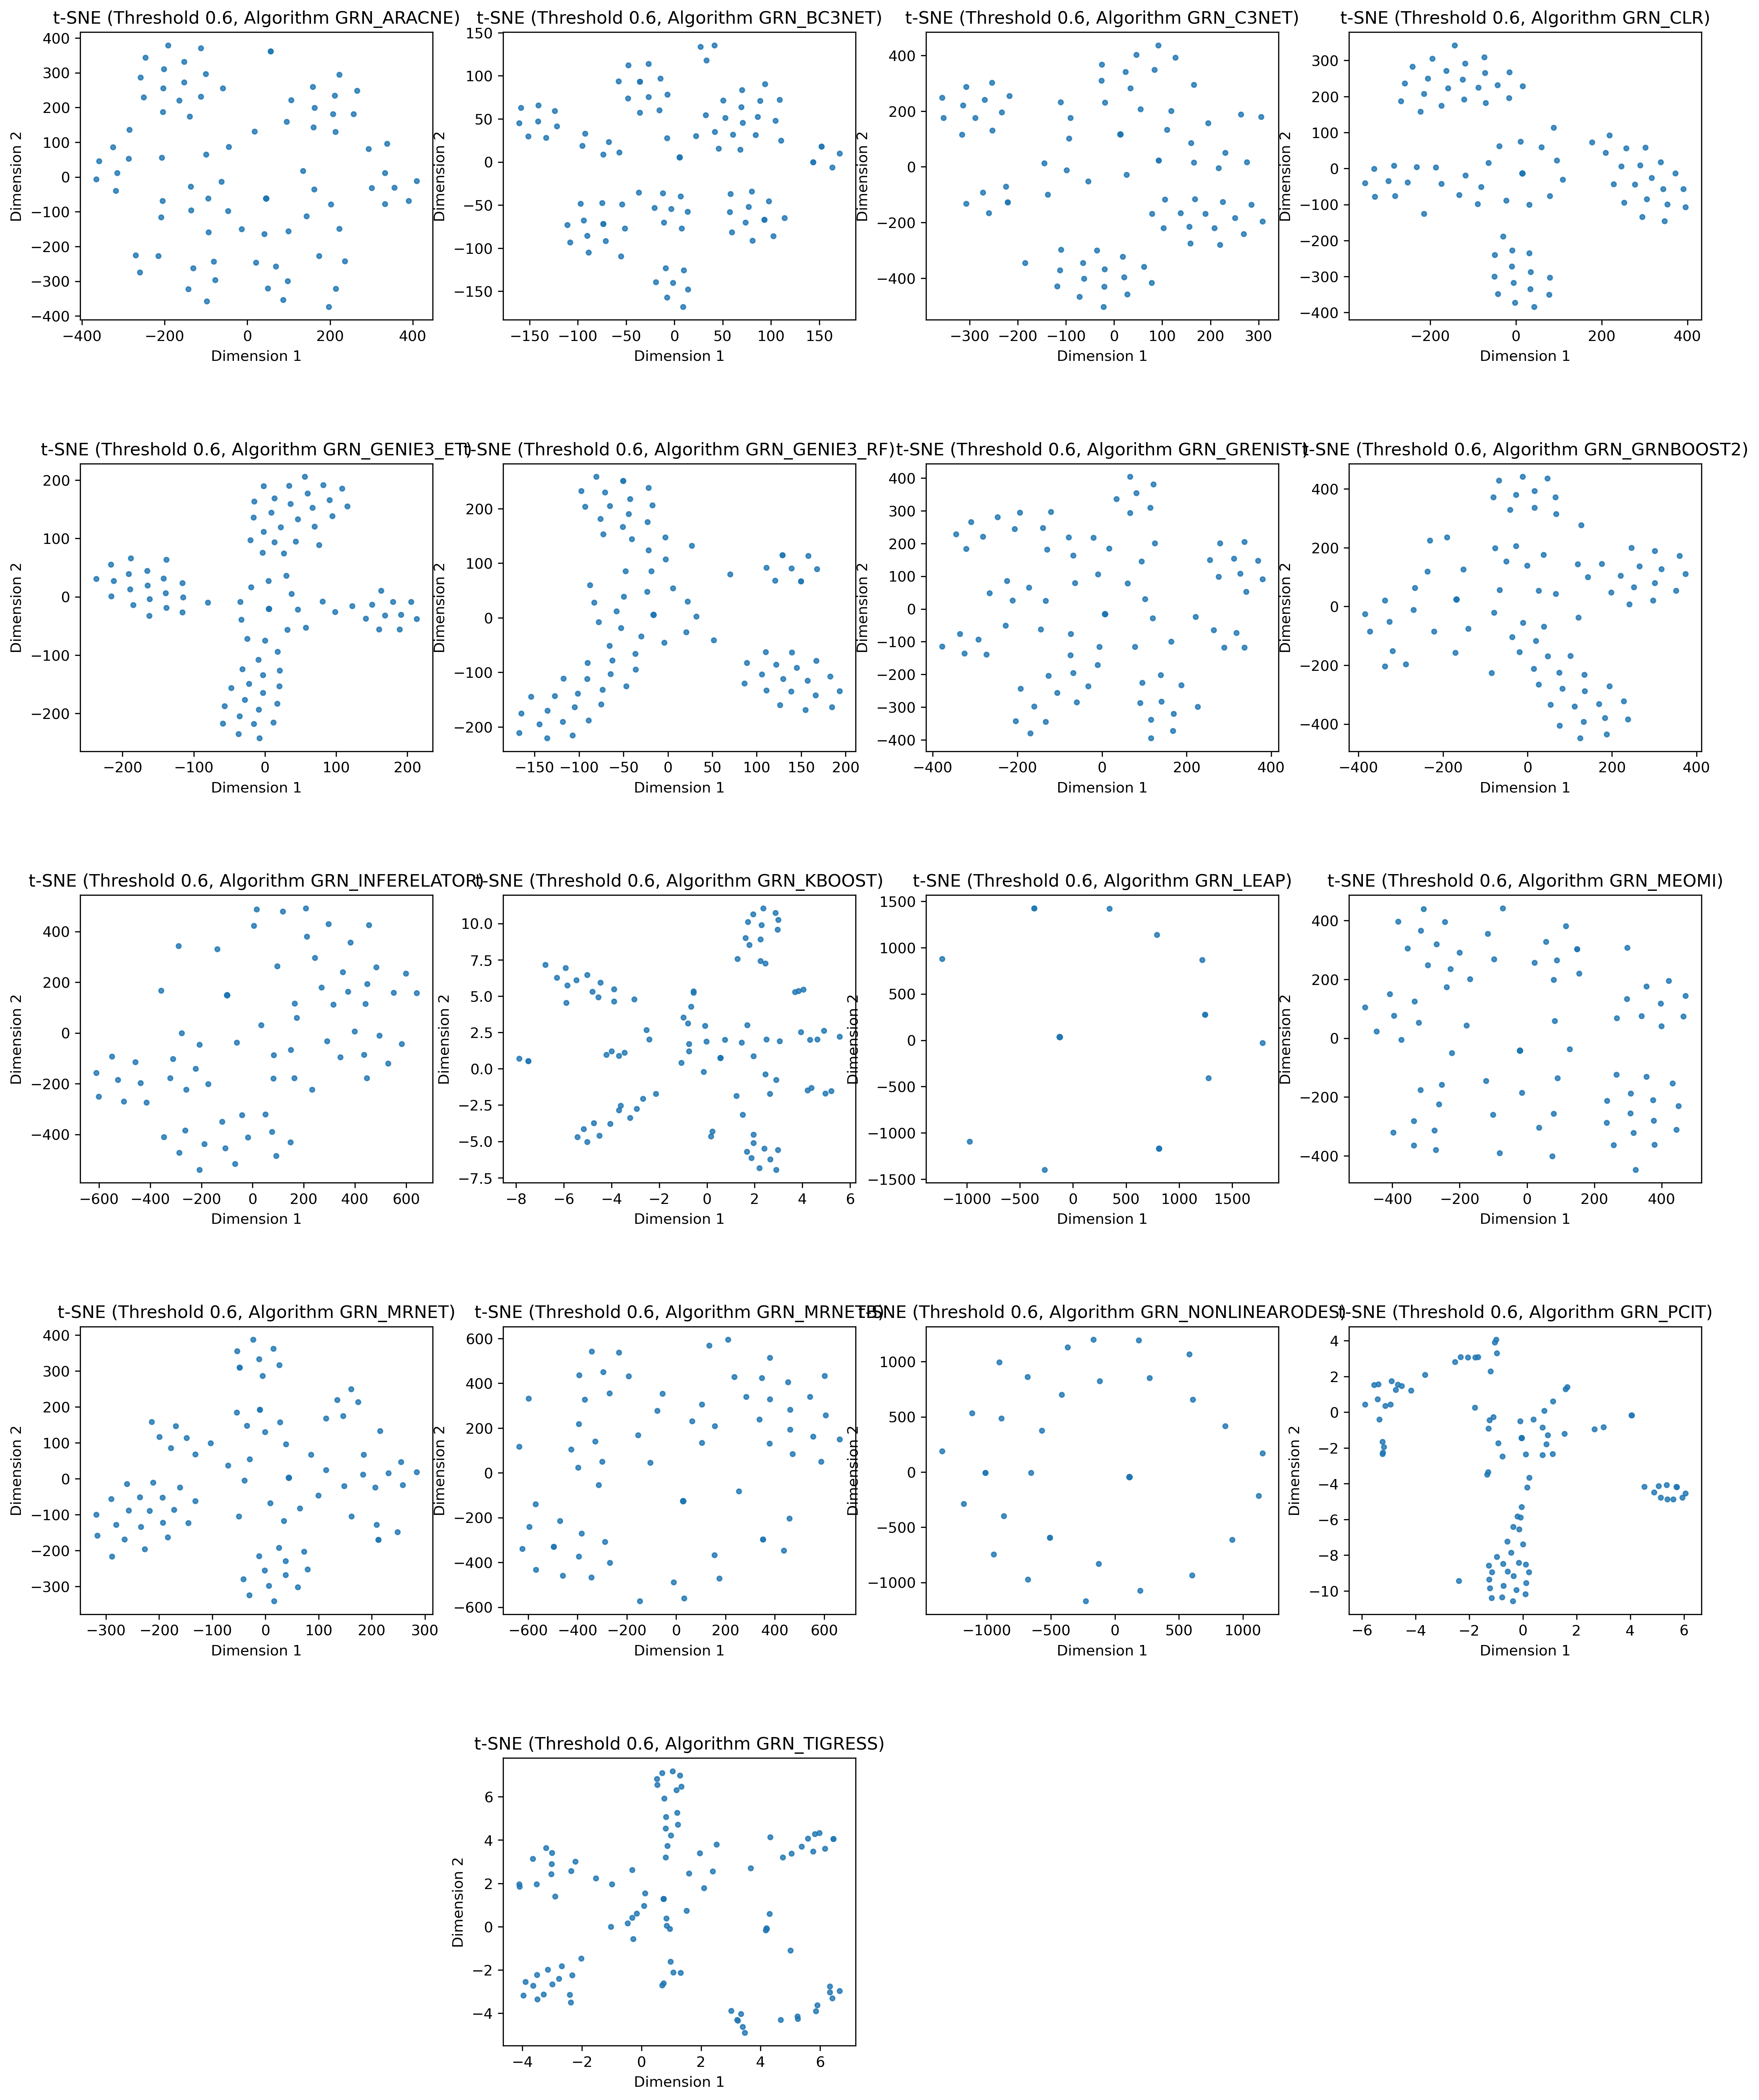
\includegraphics[width=1\textwidth]{fig/tsne_embeddings_grid_0.6.png}
    \caption{t-SNE embeddings of the dataset showing clustering patterns for different GRN algorithms using a threshold of 0.6.}
    \label{fig:tsne_embeddings}
\end{figure}

\newpage
\section{Under Objective 2}
\subsection{RATIONALE}
By employing a GCN based GRN approach, we aim to leverage the latent space representations of GCNs to integrate information from multiple algorithms, thereby providing a more robust and biologically relevant network. We test this approach on three distinct datasets: a COVID-19 RNA-seq time-series dataset, a \textit{Medicago truncatula} rhizobium module dataset, and a sorghum low-input static lipidomics dataset explained below. The goal is to validate the GCN model’s ability to outperform traditional methods in identifying key interactions, particularly those with biological significance.

\subsection{METHODS}

\subsubsection{Dataset Description}

\subsubsubsection*{COVID-19 Antiviral Response Dataset}
This dataset includes 384 patients from Massachusetts General Hospital's emergency department, 306 of whom tested positive for COVID-19, with 78 negative cases serving as controls. Blood samples from 8 healthy donors were also included. Samples were collected at Days 0 (374 samples), 3 (212 samples), and 7 (143 samples), with additional event-driven samples (44) for significant clinical changes. Disease severity was classified using the WHO COVID-19 outcome scale, with A1 and A2 as severe, and A3 to A5 as non-severe. Neutrophils were isolated via negative selection, and RNA sequencing, plasma proteomics, and antibody profiling were performed to study neutrophil dynamics \cite{covid}.

\subsubsubsection*{\textit{Medicago truncatula} Rhizobium Module Dataset} 
This dataset examines transcriptional dynamics during early nodulation in \textit{Medicago truncatula} in response to \textit{Sinorhizobium medicae}. Time-series RNA-Seq was conducted on shoot and root tissues over 72 hours, with samples collected at 0, 12, 24, 48, and 72 hours post-inoculation. Using the GeneShift computational workflow, dynamic changes in gene expression were identified without averaging replicates, revealing both known and novel genes involved in nodulation and defense responses \cite{medicago}.

\subsubsubsection*{Sorghum Low-Input Static Lipidomics Dataset}
Around 400 Sorghum Association Panel lines \cite{sap} were grown in Florence, SC, under low nitrogen, low phosphorus, and early planting conditions (cold stress). Leaf samples were collected at the V6 stage for lipidomics analysis, conducted in collaboration with the Joint Genome Institute (JGI) \cite{jgi_genome_portal}. Approximately 150 unique lipids were identified. A linear mixed model GWAS was run for each lipid using SAP genotypes, and the top genes from these analyses were tabulated. This dataset is not a time series expression data. However, some of the algorithms we used are able to handle single replicate multiple condition dataset. So, each genotype here will act as a new condition. 



\subsubsection{Model Application}

\subsubsubsection*{COVID-19 Antiviral Response Dataset}

Using a threshold of 0.6 and common interactions across more than eight algorithms, the GCN GRN identified critical interactions among \texttt{OAS1}, \texttt{OAS3}, \texttt{DDX60}, and \texttt{MX1}, as well as between \texttt{DHX58} and \texttt{ISG15} (Fig.~\ref{fig:COVID_GRN}). These interactions align with existing literature, underscoring their roles in antiviral responses, particularly in the context of COVID-19.

\begin{figure}[h!]
\centering

% COVID Raw
\begin{subfigure}[b]{0.16\textwidth} % Adjust width as needed
    \centering
    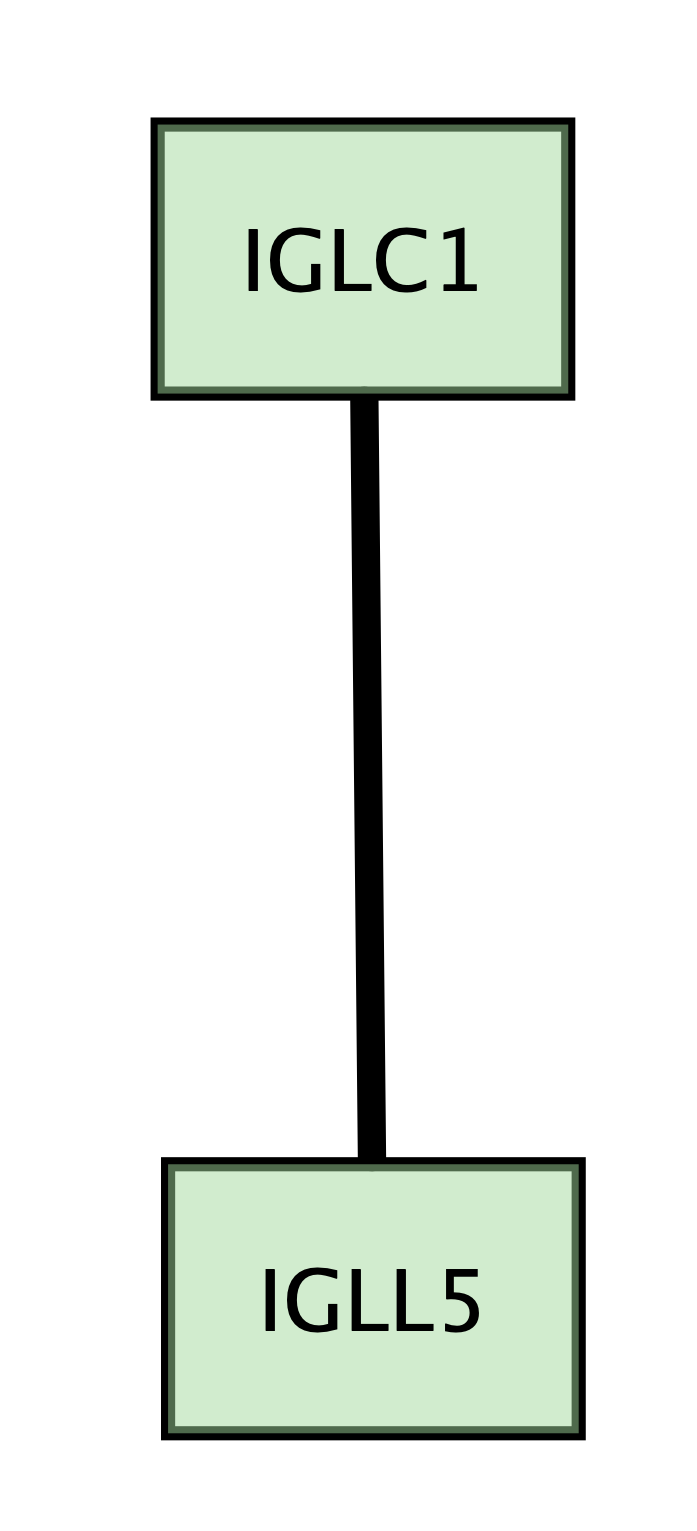
\includegraphics[width=\linewidth]{fig/COVID_raw.png}
    \caption{COVID Raw GRN}
    \label{fig:covid_raw}
\end{subfigure}
\hfill
% COVID GCN
\begin{subfigure}[b]{0.48\textwidth}
    \centering
    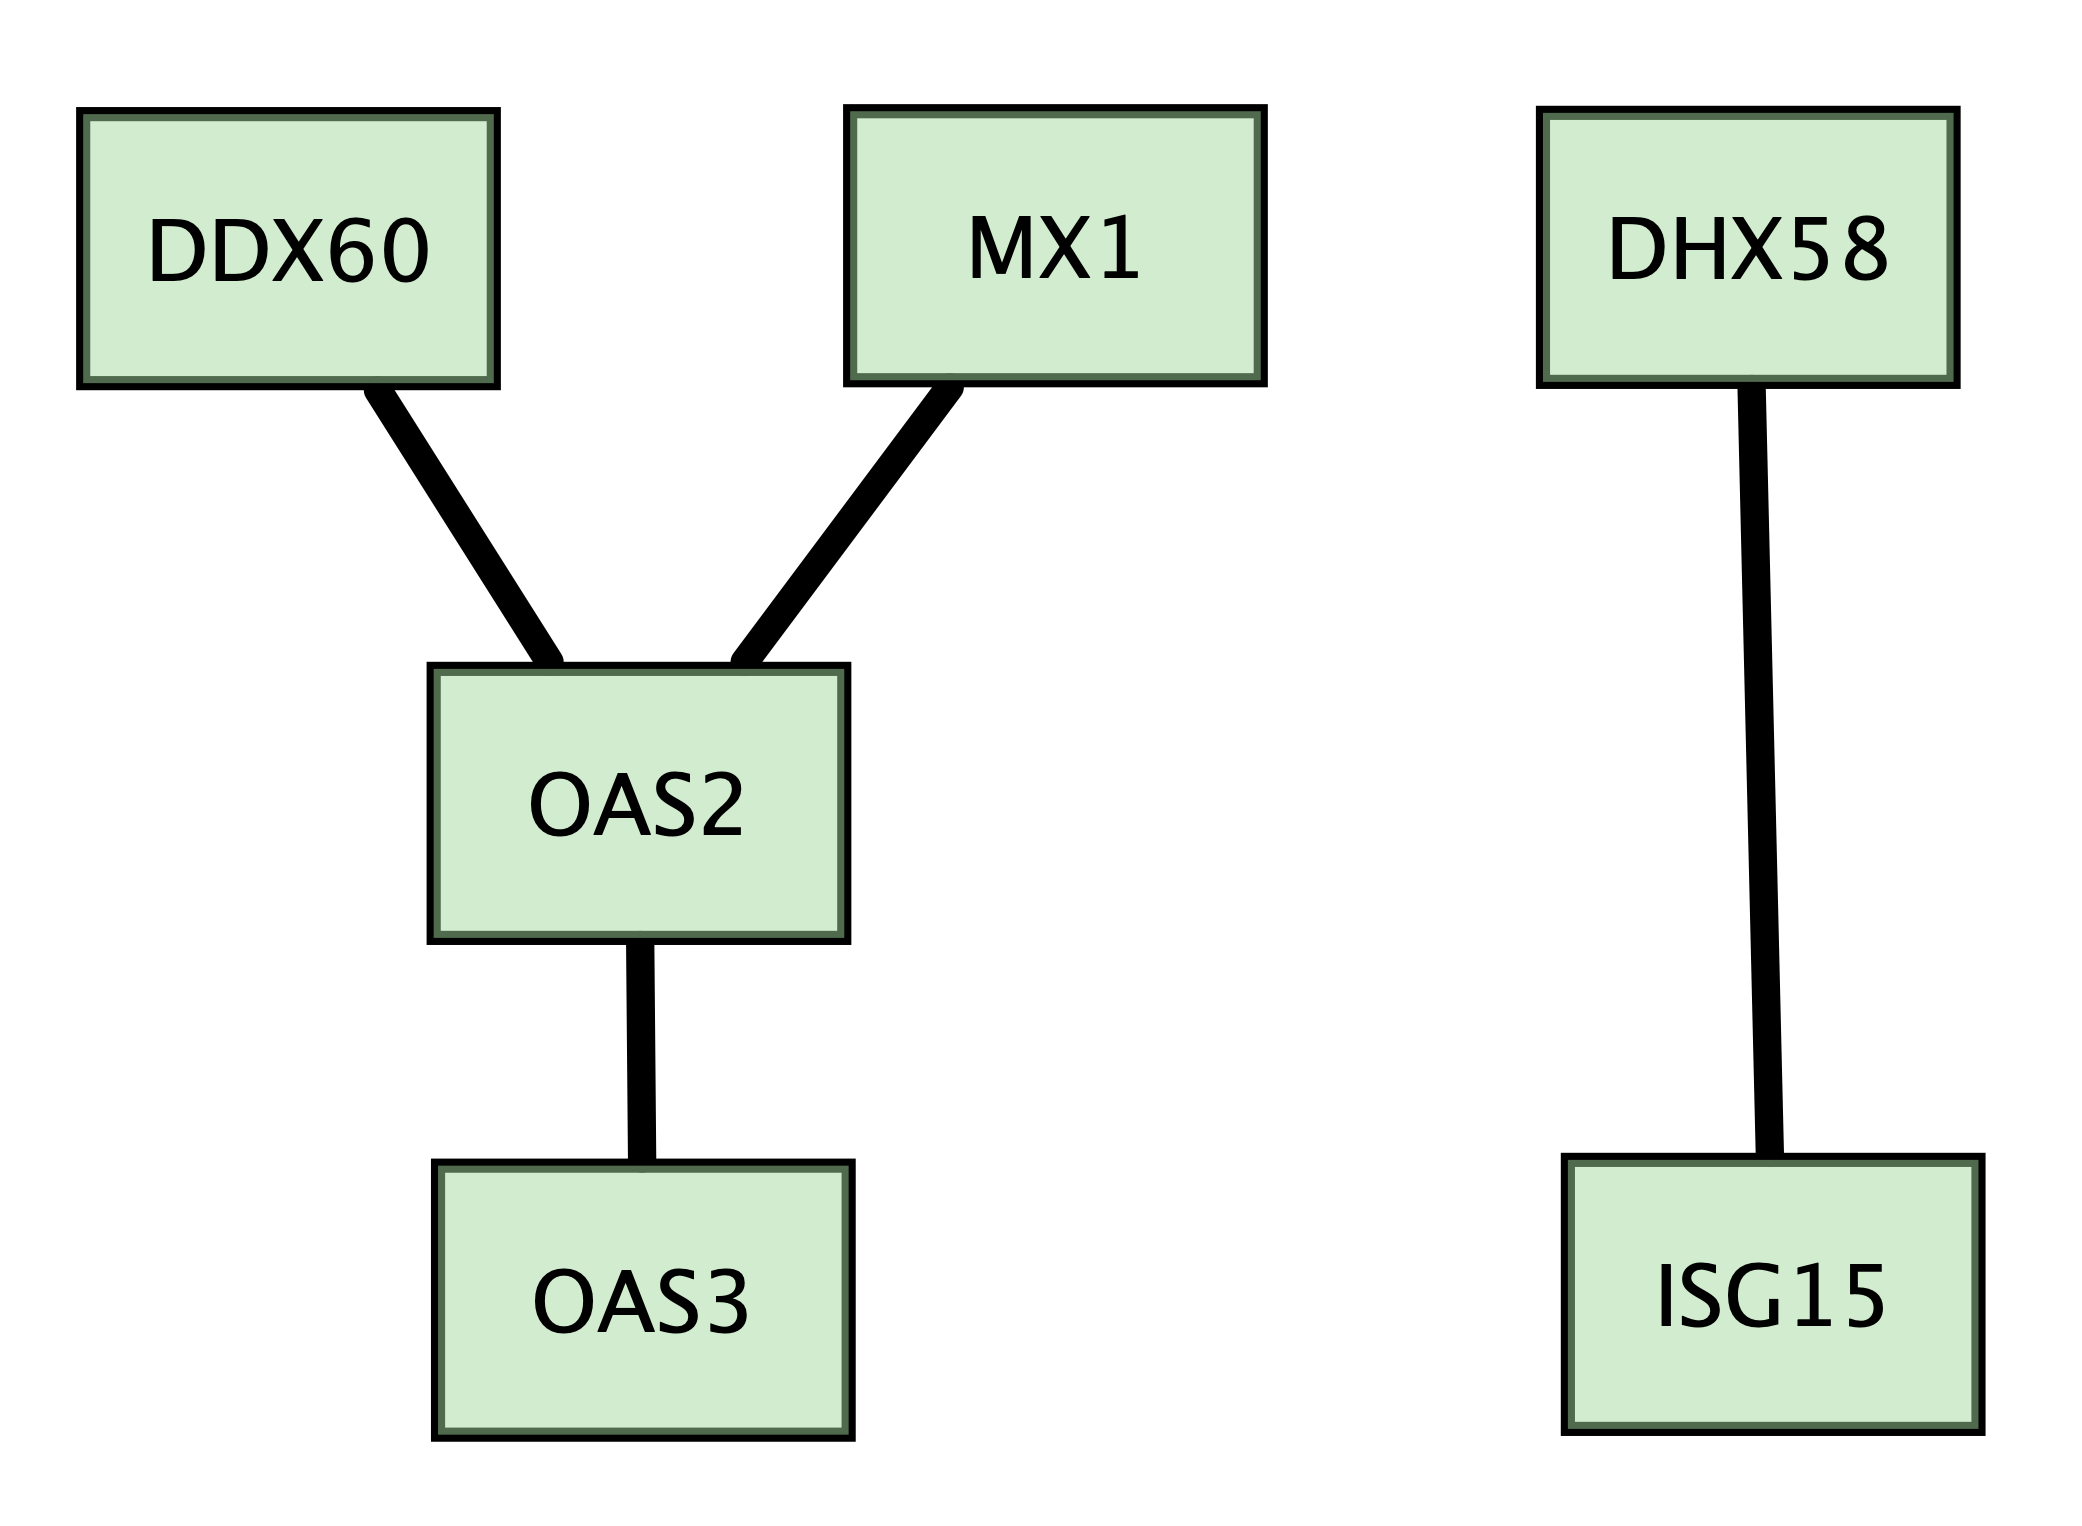
\includegraphics[width=\linewidth]{fig/COVID_GCN.png}
    \caption{COVID GCN GRN}
    \label{fig:covid_gcn}
\end{subfigure}

\caption{Comparison of raw and GCN-based GRNs for the COVID dataset derived from GRN analyses. (a) Raw GRN (b) GCN-derived GRN.}
\label{fig:COVID_GRN}
\end{figure}


\texttt{OAS2} and \texttt{OAS3} play a role in the innate immune response, synthesizing 2',5'-oligoadenylates (2-5As) that activate latent RNase L. This activation degrades viral RNA and inhibits viral replication \cite{schwartz2019rna}. Furthermore, \texttt{OAS2} and \texttt{OAS3} are critical components of the host-pathogen interaction pathway for human coronaviruses, particularly in interferon induction (Fig.~\ref{fig:Host_Pathogen_Interaction}) \cite{hancks2015overlapping}. \texttt{DDX60} encodes a DEXD/H box RNA helicase that functions as an antiviral factor, amplifying RIG-I-like receptor-mediated signaling, a key pathway in RNA sensing and immune regulation \cite{tapescu2024ddx}. Similarly, \texttt{MX1}, a GTP-metabolizing protein, is a well-established player in cellular antiviral responses and cytokine signaling, further demonstrating the biological relevance of the identified interactions \cite{ashley2019interferon}. From the STRING interaction network \cite{vonmering2003string}for Host-pathogen interaction of human coronaviruses - interferon induction (Fig.~\ref{fig:STRING_COVID_network}), using very high confidence filtering (\(> 0.9\)), we identified interactions among \texttt{OAS2}, \texttt{OAS3}, \texttt{DDX58}, and \texttt{MX1}. For more information on the host-pathogen interaction of human coronaviruses with interferon induction, refer to the PathCards database: \href{https://pathcards.genecards.org/card/host-pathogen_interaction_of_human_coronaviruses_-_interferon_induction}{Host-Pathogen Interaction of Human Coronaviruses - Interferon Induction}.

\begin{figure}[h!]
    \centering
    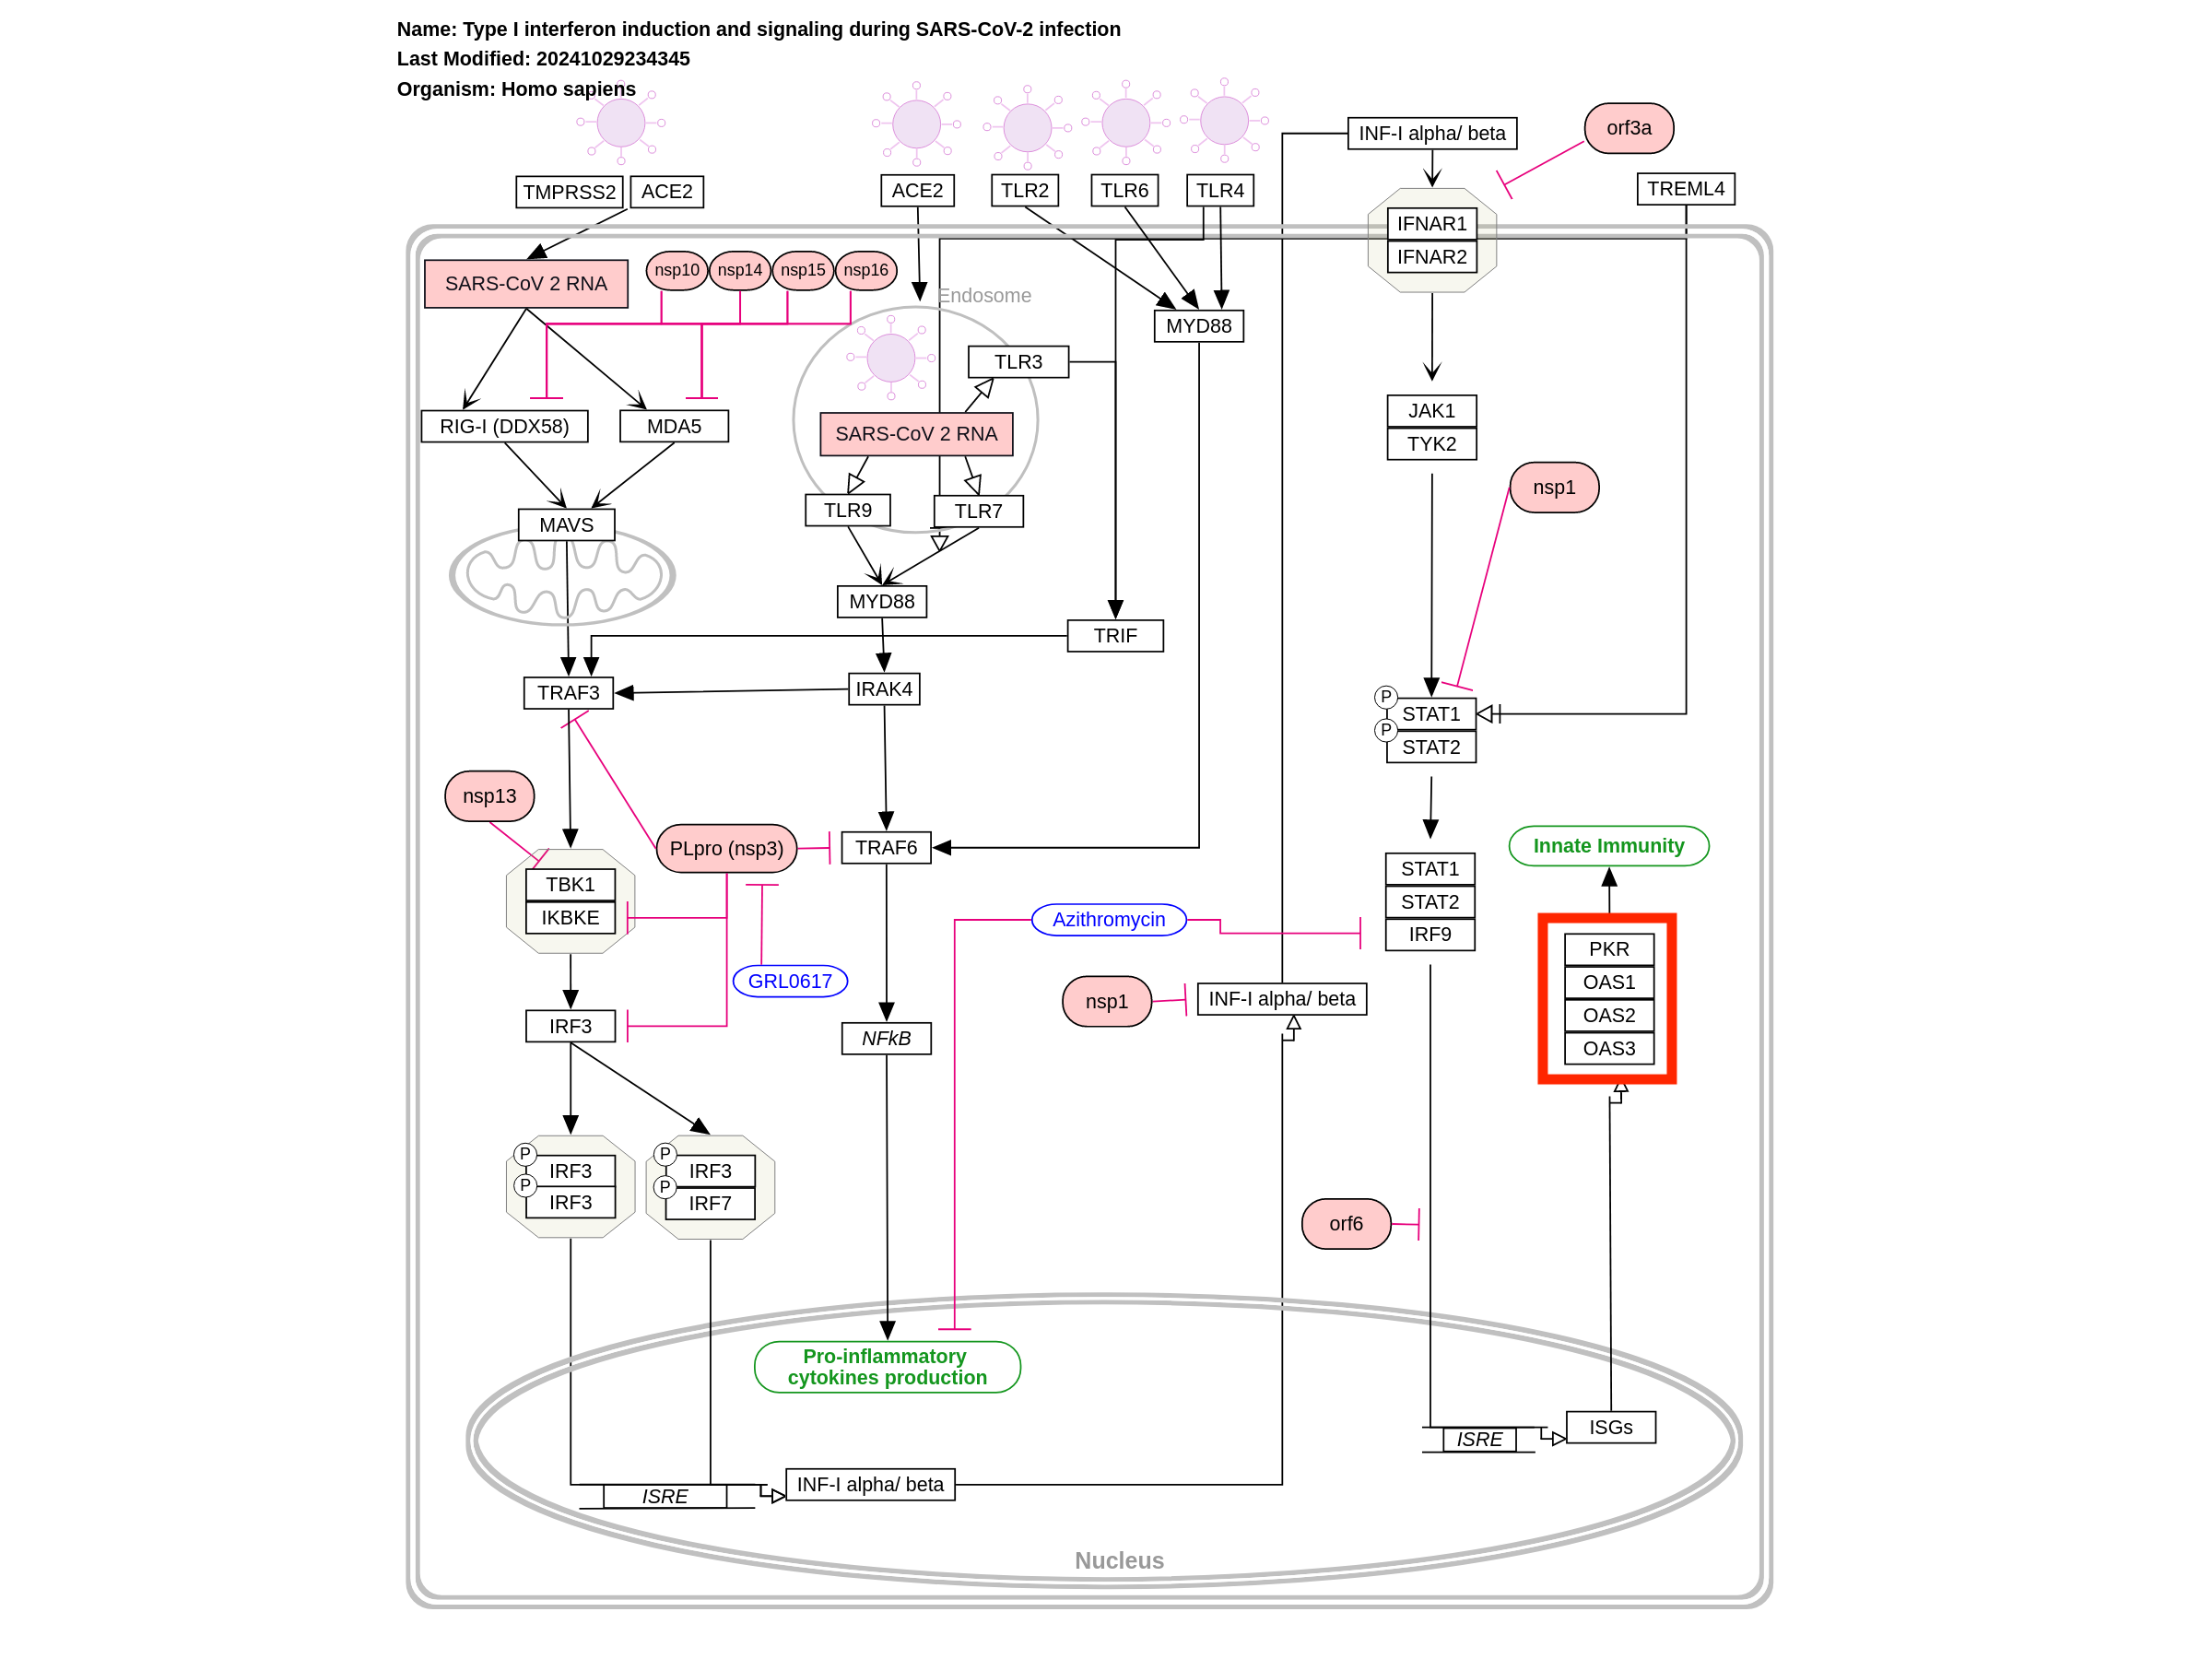
\includegraphics[width=1\textwidth]{fig/Host-pathogen interaction of human coronovirus-interferon induction.png} % Adjust the path as needed
    \caption{Host-Pathogen Interaction: This figure illustrates the interaction between human coronavirus and interferon induction pathways. Genes identified through GCN-GRN involved in the regulation of the antiviral response are highlighted in red boxes.}
    \label{fig:Host_Pathogen_Interaction}
\end{figure}

\begin{figure}[h!]
    \centering
    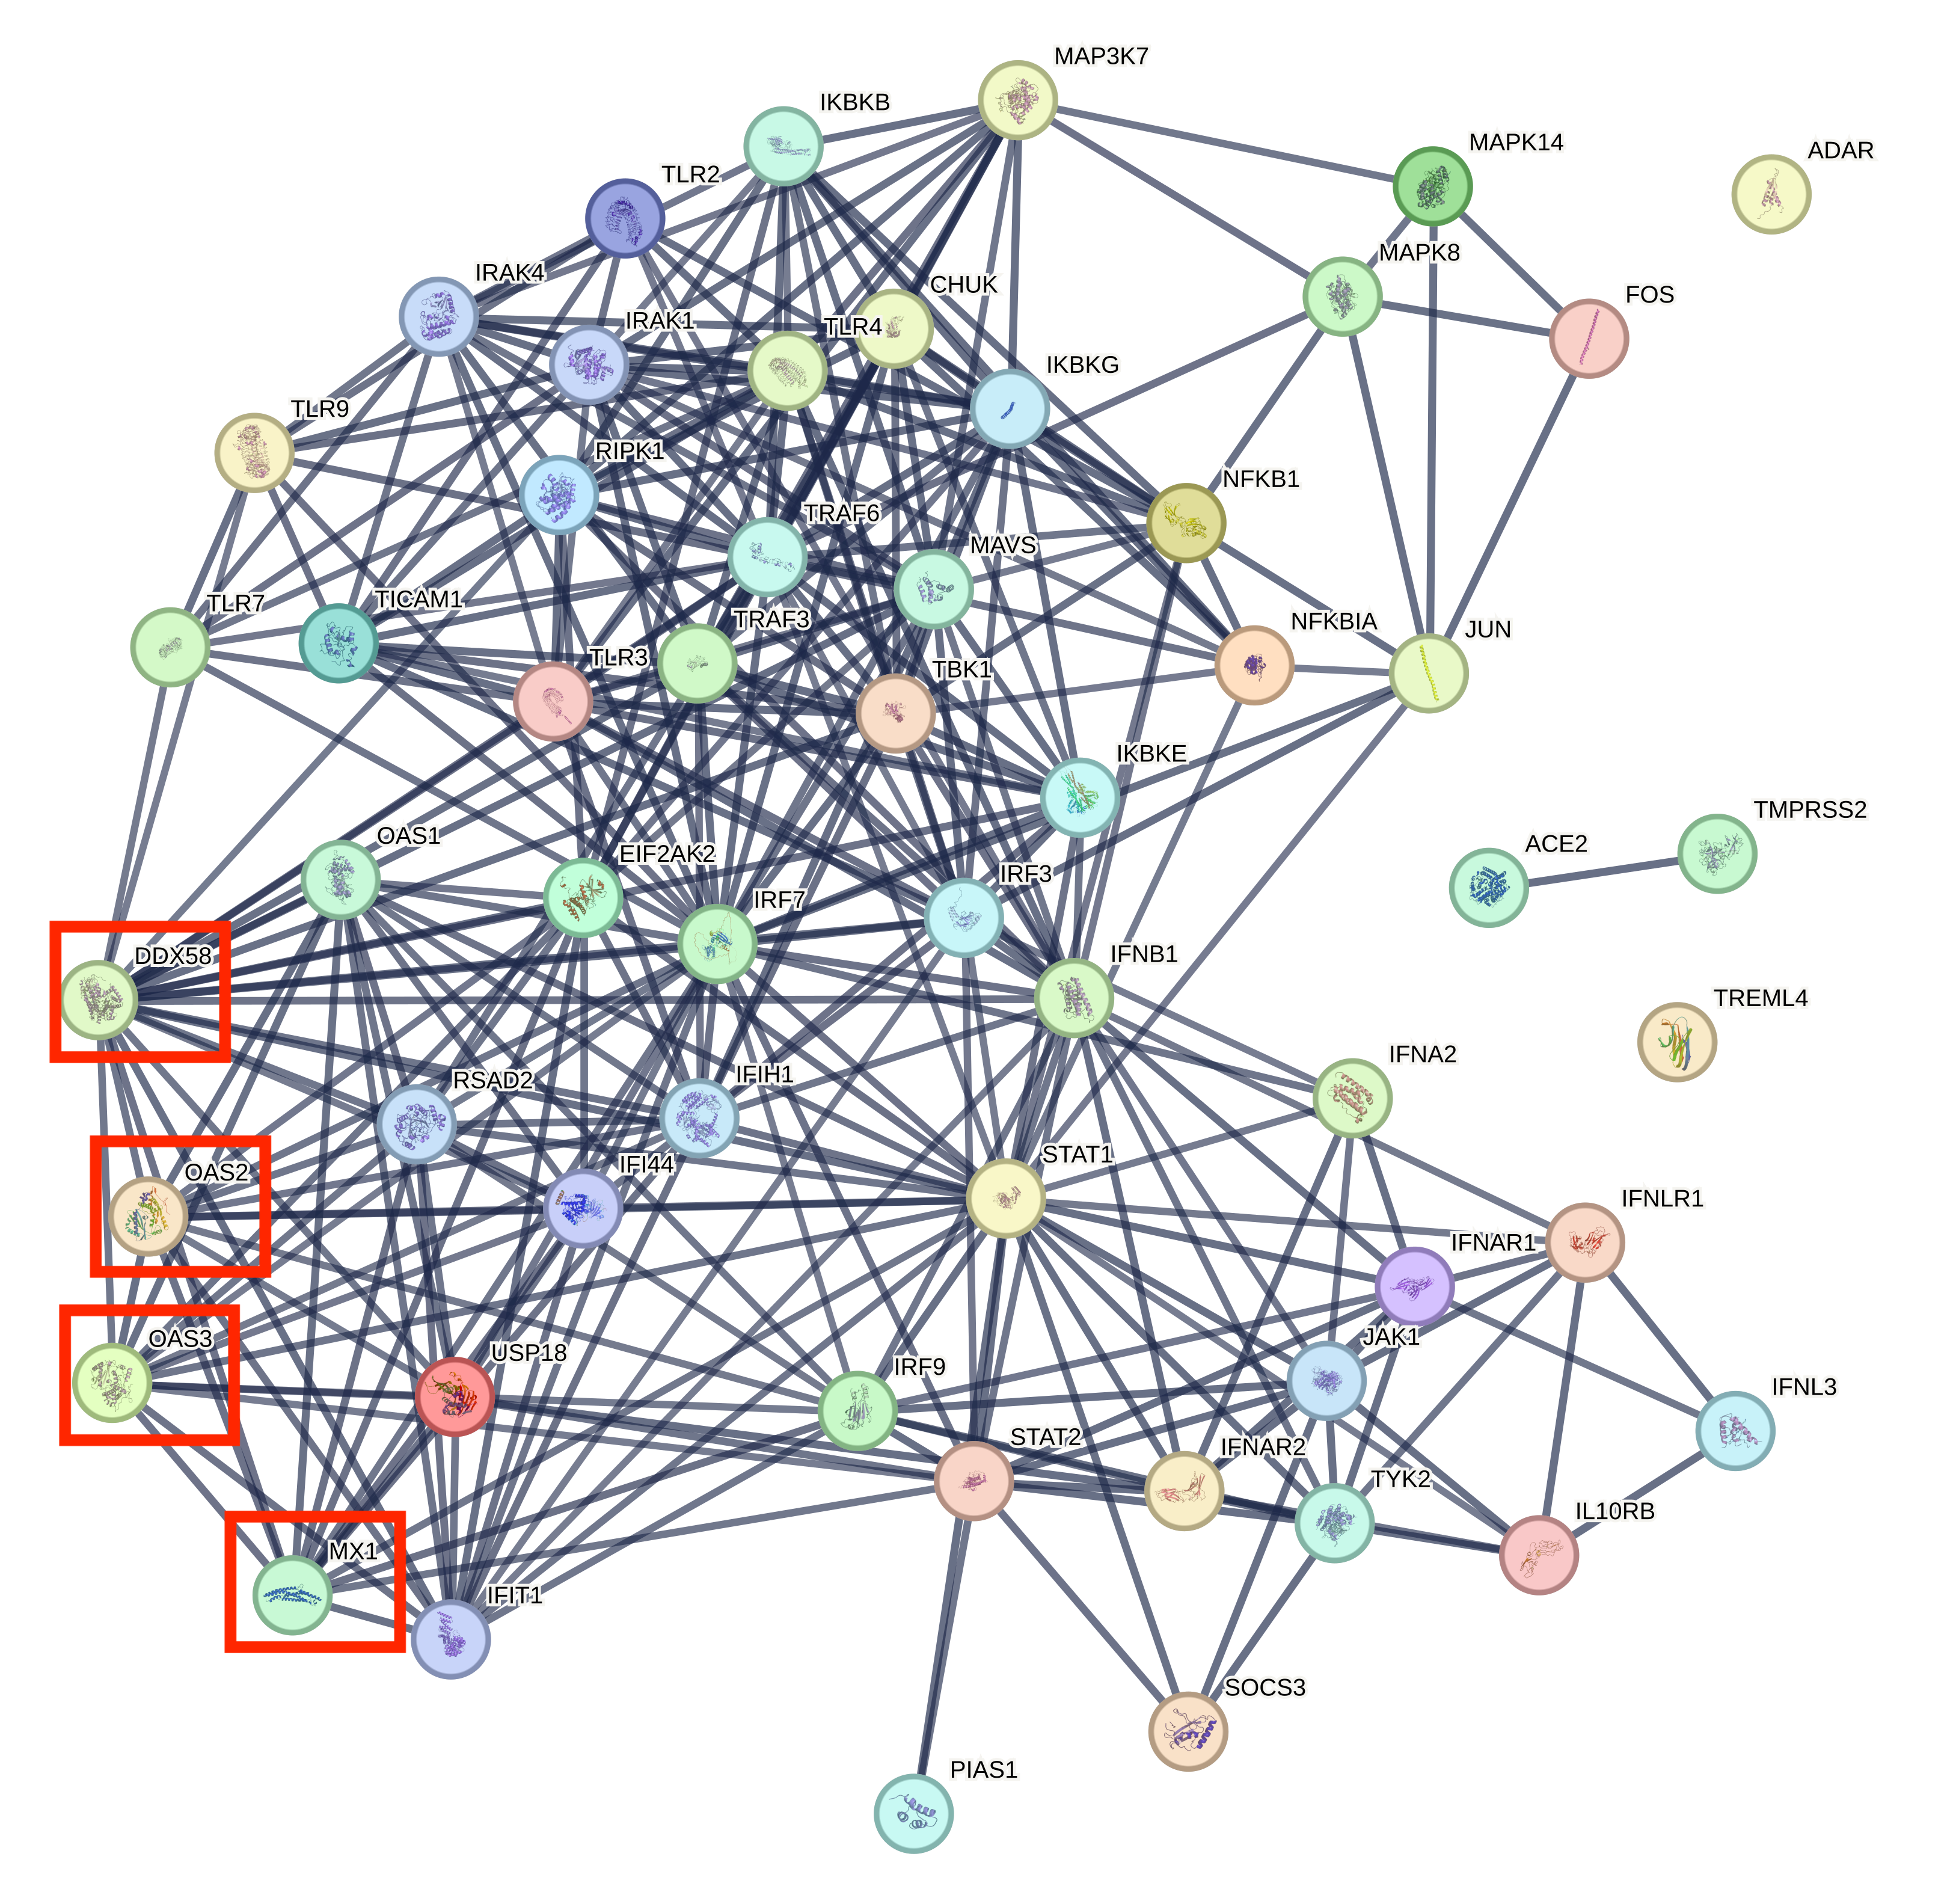
\includegraphics[width=1\textwidth]{fig/STRING_1st_network_COVID.png} % Adjust the path as needed
    \caption{Interaction network for Host-Pathogen Interaction of Human Coronaviruses - Interferon Induction using STRING. The genes identified throught GCN-GRN are represented in red square boxes.}
    \label{fig:STRING_COVID_network}
\end{figure}


\texttt{DHX58} contributes to the negative regulation of type I interferon production and overall defense responses, highlighting the balance between effective antiviral responses and immune regulation \cite{delang2020interferon}. Finally, \texttt{ISG15}, an interferon-stimulated gene, exhibits antiviral activity during viral infections and mediates cell-to-cell signaling \cite{sarkar2023isg15}. From the SARS-CoV-2 infection pathway (highlighted in red circles), we also observe that \texttt{ISG15} and \texttt{DHX58} form an \texttt{ISG15:DHX58} conjugate, acting as a repressor during viral infection (Fig.~\ref{fig:Second_Pathway}).

\begin{figure}[h!]
    \centering
    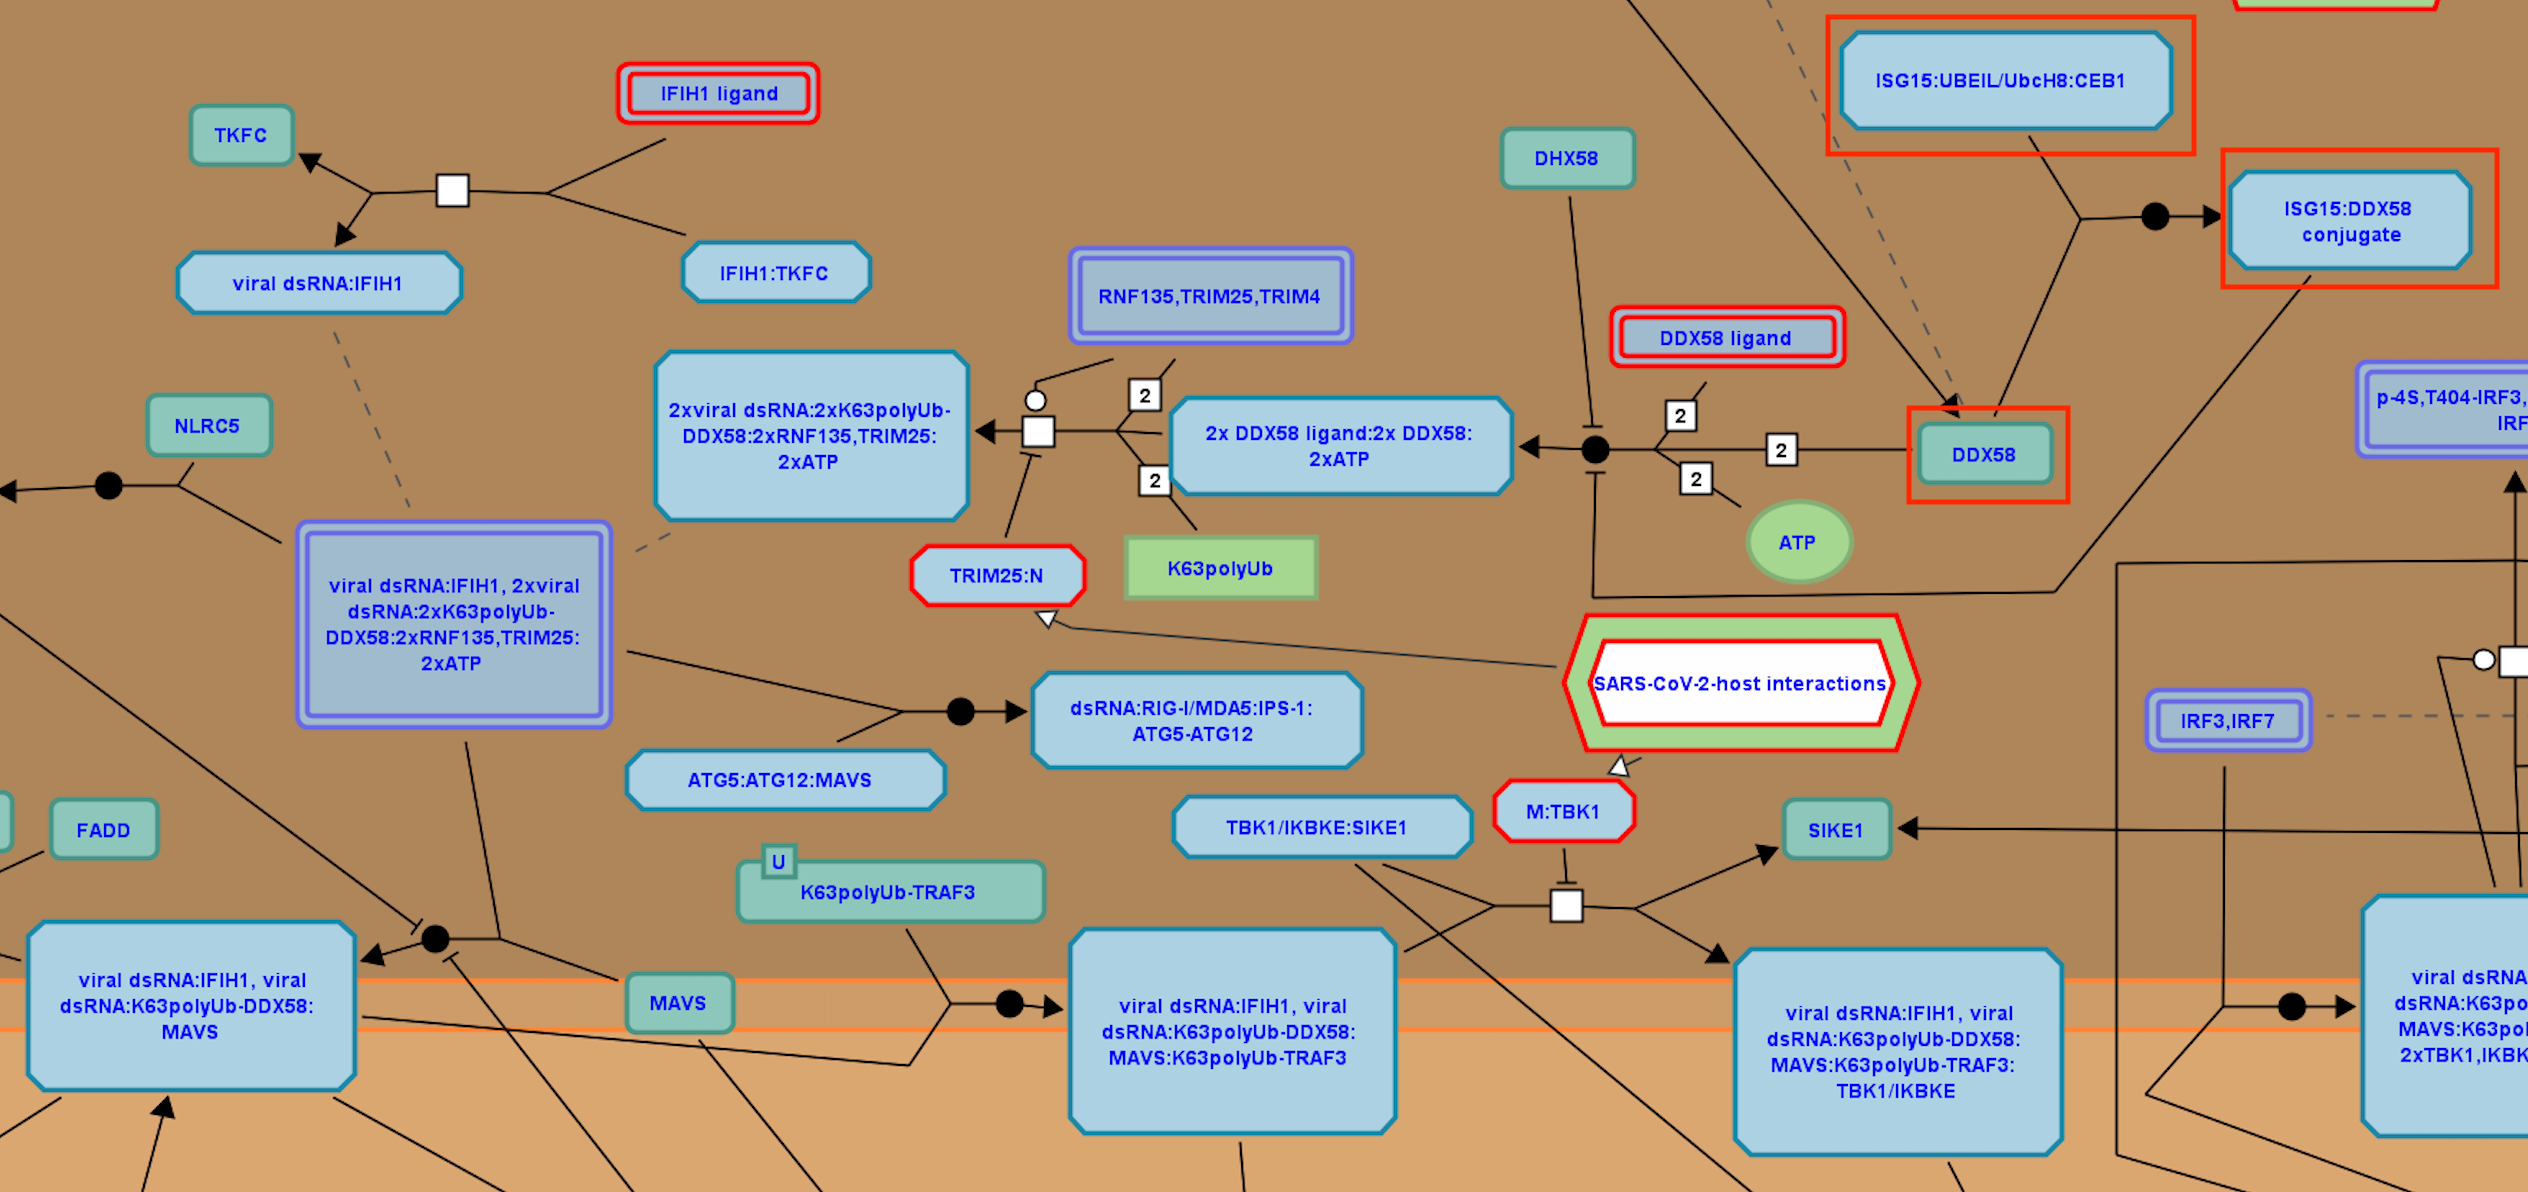
\includegraphics[width=0.8\textwidth]{fig/second_pathway_cropped.png} % Adjust the path as needed
    \caption{ \href{https://reactome.org/PathwayBrowser/#/R-HSA-168928&SEL=R-HSA-936557}{Reactome pathway representing SARS-CoV-2-host interactions}. The genes highlighted in single red boxes represents the GCN-derived GRNs. Here, \texttt{DDX58} intearcts with \texttt{ISG15} to produce a \textbf{ISG15:DDX58 conjugate}}
    \label{fig:Second_Pathway}
\end{figure}


These findings underscore the GCN GRN's capacity to uncover biologically meaningful interactions, particularly those with high experimental evidence supporting their roles in antiviral mechanisms. The identified interactions between key immune-related genes, such as \textit{OAS1}, \textit{OAS3}, \textit{DDX60}, and \textit{MX1}, align with established literature, highlighting their pivotal roles in host-pathogen interactions. By revealing these relationships, the model not only enhances our understanding of the innate immune response but also points toward potential therapeutic targets for combating COVID-19.

Additionally, the raw GRN analysis uncovered interactions involving \textit{IGLC1} and \textit{IGLL5}, which, while less obvious, may still play a significant role in immune defense. \textit{IGLC1} is predicted to enable antigen binding and immunoglobulin receptor activity, facilitating immune activation, defense against pathogens, and phagocytosis. Similarly, \textit{IGLL5} encodes an immunoglobulin lambda-like polypeptide associated with antigen binding \cite{safran2010genecards}. These genes, though not immediately prominent in antiviral pathways, highlight the importance of considering interactions that may not meet stringent filtering thresholds. Lowering the filtering threshold could include other potentially significant genes, but it would also result in an increased number of nodes and edges, complicating the task of selecting the most relevant interactions for further investigation.

Thus, while stringent thresholds help to prioritize high-confidence interactions, striking a balance between sensitivity and specificity remains critical. The GCN GRN’s ability to integrate and refine data across multiple algorithms provides a promising framework to address these challenges, enabling a well rounded regulatory interactions in gene networks.

\begin{table}[h!]
\centering
\caption{Genes identified through GRN adapted from GeneCards (\url{https://www.genecards.org/}).}
\begin{tabular}{|l|p{6cm}|p{6cm}|}
\hline
\textbf{Gene Name} & \textbf{Function} & \textbf{Pathways Associated} \\ \hline
\texttt{DDX60} & Encodes a DEXD/H box RNA helicase that functions as an antiviral factor and promotes RIG-I-like receptor-mediated signaling. & NA \\ \hline
\texttt{MX1} & Encodes a guanosine triphosphate (GTP)-metabolizing protein that participates in the cellular antiviral response. & Antiviral mechanism by IFN-stimulated genes; cytokine signaling in the immune system. \\ \hline
\texttt{OAS2} & Involved in the innate immune response to viral infection; synthesizes 2',5'-oligoadenylates (2-5As) that activate latent RNase L, degrading viral RNA and inhibiting viral replication. & Antiviral mechanism by IFN-stimulated genes; host-pathogen interaction of human coronaviruses. \\ \hline
\texttt{OAS3} & Inhibition of cellular protein synthesis and viral infection resistance. Plays roles in apoptosis, cell growth, differentiation, and gene regulation. Synthesizes 2',5'-oligoadenylates (2-5As) from ATP, activating ribonuclease L, leading to RNA degradation and inhibition of protein synthesis. & Antiviral mechanism by IFN-stimulated genes; host-pathogen interaction of human coronaviruses; interferon induction. \\ \hline
\texttt{DHX58} & Involved in the negative regulation of defense response and type I interferon production. & Innate immune system; DDX58/IFIH1-mediated induction of interferon-alpha/beta. \\ \hline
\texttt{ISG15} & Encodes a protein with chemotactic activity towards neutrophils, directs ligated target proteins to intermediate filaments, mediates cell-to-cell signaling, and exhibits antiviral activity during viral infections. & SARS-CoV-2 infection; translesion synthesis by Y family DNA polymerases bypassing lesions on DNA template. \\ \hline
\texttt{IGLC1} & Predicted to enable antigen binding activity and immunoglobulin receptor binding activity, activating the immune response, defense response to other organisms, and phagocytosis. & NA \\ \hline
\texttt{IGLL5} & Encodes one of the immunoglobulin lambda-like polypeptides related to antigen binding. & NA \\ \hline
\end{tabular}
\label{tab:grn_genes}
\end{table}

\subsubsubsection*{\textit{Medicago truncatula} Rhizobium Module Dataset} 
For this dataset, gene clustering for roots was performed using the \texttt{geneshift} algorithm \cite{medicago}. A threshold of 0.6 was applied, and interactions shared by at least six algorithms were selected. Within the roots cluster, notable connections were identified, including \texttt{Medtr4g088265}, \texttt{Medtr4g094352}, and \texttt{Medtr2g103317}, with the first two genes linked to nodulin function. Another significant interaction connected an early nodulin gene (\texttt{Medtr7g065770}) to a salt response/antifungal domain protein gene (\texttt{Medtr3g415620}) (Fig.~\ref{fig:Nitrogen_GRN}) \cite{boschiero2020mtsspdb}.

Diana I. Trujillo \textit{et al.} \cite{trujillo2019nodule} conducted an experiment with a 19.4-kb segment deletion in the \textit{npd1/2/3/4/5-1} mutant line of \textit{Medicago truncatula}. The \textit{NPD} genes, or Nodule-specific Polycystin-1, Lipoxygenase, Alpha Toxin domain proteins, represent a family of nodule-specific proteins that have expanded exclusively in the \textit{Medicago} lineage of legumes. These proteins play a crucial role in nodulation, facilitating the symbiotic relationship between legumes and rhizobia for effective nitrogen fixation \cite{pislariu2019npd1}. This 19.4-kb segment deletion encompassed multiple genes, including \texttt{Medtr2g103317}. The study revealed that mutant plants exhibited smaller and largely ineffective nodules compared to the wild type (WT). While it is difficult to attribute these phenotypic effects to \texttt{Medtr2g103317} alone due to the presence of other deleted genes, its role within this genomic region warrants further investigation. 

Additionally, \texttt{Medtr4g094352}, encoding the MtN21 protein, was initially described as a nodulin induced during \textit{R. meliloti}–\textit{M. truncatula} symbiosis \cite{gamas1996subtractive}. These interactions and connections underscore the potential significance of \texttt{Medtr2g103317} and \texttt{MtN21} in the broader context of symbiotic nitrogen fixation.

Within our GRN analysis, \texttt{Medtr2g103317} interacts with key regulators such as \texttt{MtN21/MtUMAMIT14} and \texttt{Nodule Cysteine Rich} (NCR) genes, which are vital for nodule development and function \cite{boschiero2020mtsspdb}. Although \texttt{Medtr2g103317} remains uncharacterized, indirect evidence suggested it may play a role in nodule formation. By leveraging the GCN model, we observe that \texttt{Medtr2g103317} clusters with known nodule-associated genes, providing a degree of confidence on Trujillo's results that it might contribute to nodulation processes.

The early noduline gene (\texttt{Medtr7g065770}) \cite{journet2001medicago} connecting to a salt response/antifungal domain protein gene (\texttt{Medtr3g415620}) represents a direct link between experimental observations and computational results. These findings underscore the GCN model's ability to uncover biologically relevant gene interactions and connections that align with experimental data, providing valuable insights into nitrogen fixation and nodule function.

Similar to the COVID-19 raw GRN, the GRNs generated lack a clear connection to the specific experiment at hand. This highlights the significance of the relevant interactions identified by the GCN model, which enhances the precision of our analysis.

\begin{figure}[h!]
\centering

% medicavo Raw
\begin{subfigure}[b]{0.48\textwidth} % Adjust width as needed
    \centering
    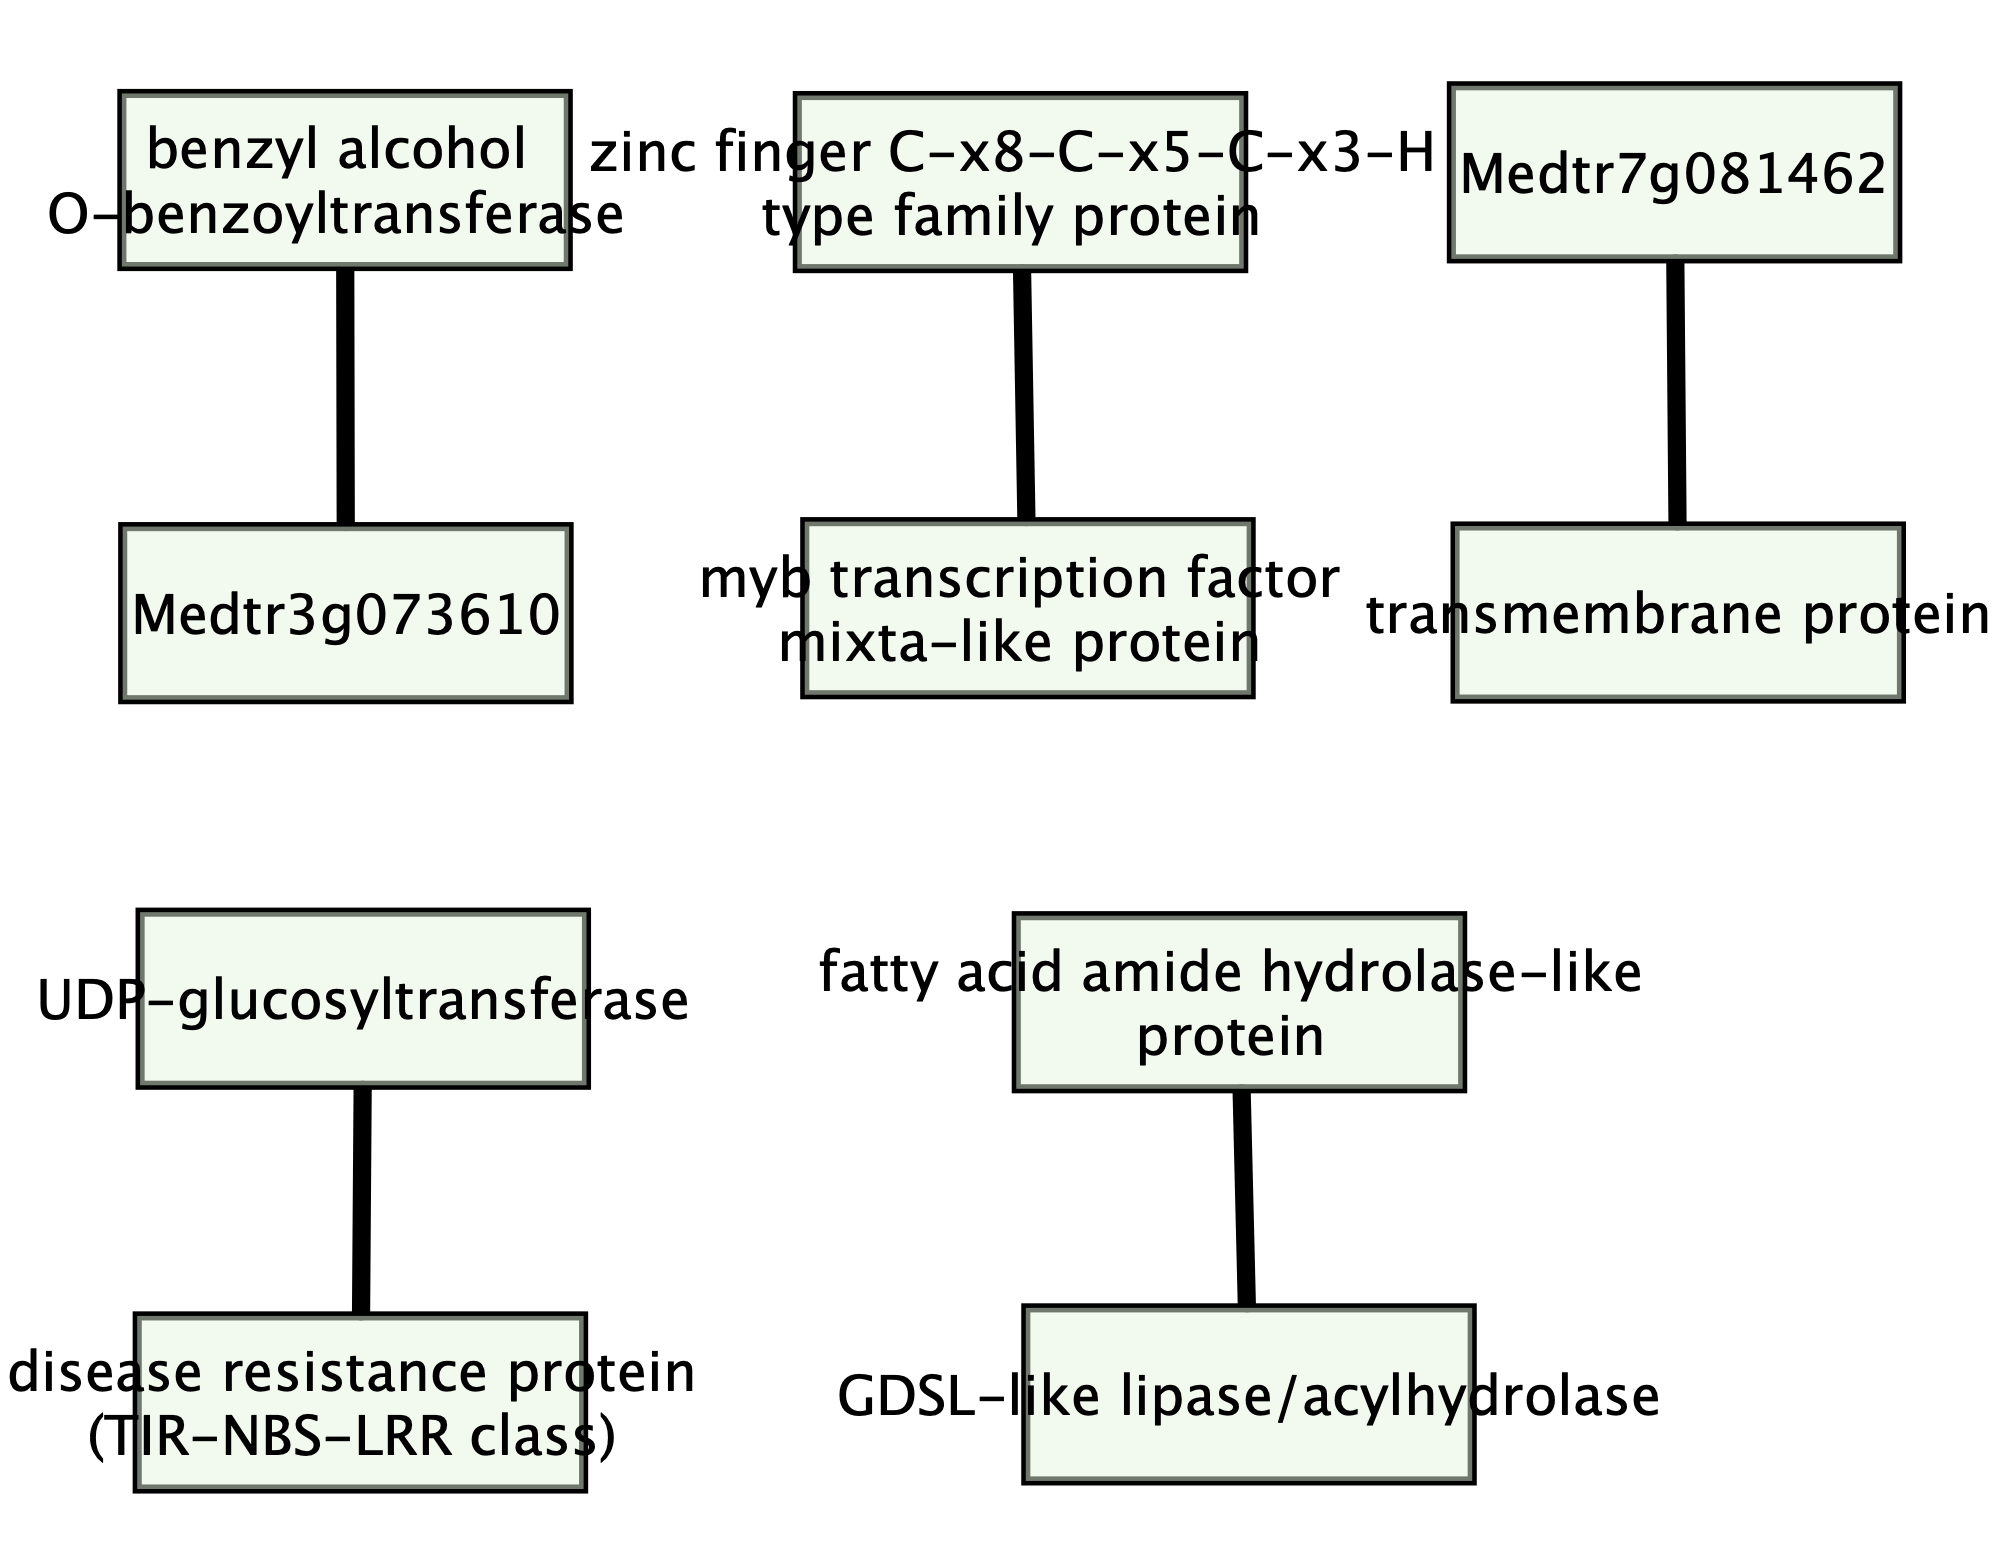
\includegraphics[width=\linewidth]{fig/Nitrogen_raw.png}
    \caption{Roots Raw GRN}
    \label{fig:nitrogen_raw}
\end{subfigure}
\hfill
% COVID GCN
\begin{subfigure}[b]{0.48\textwidth}
    \centering
    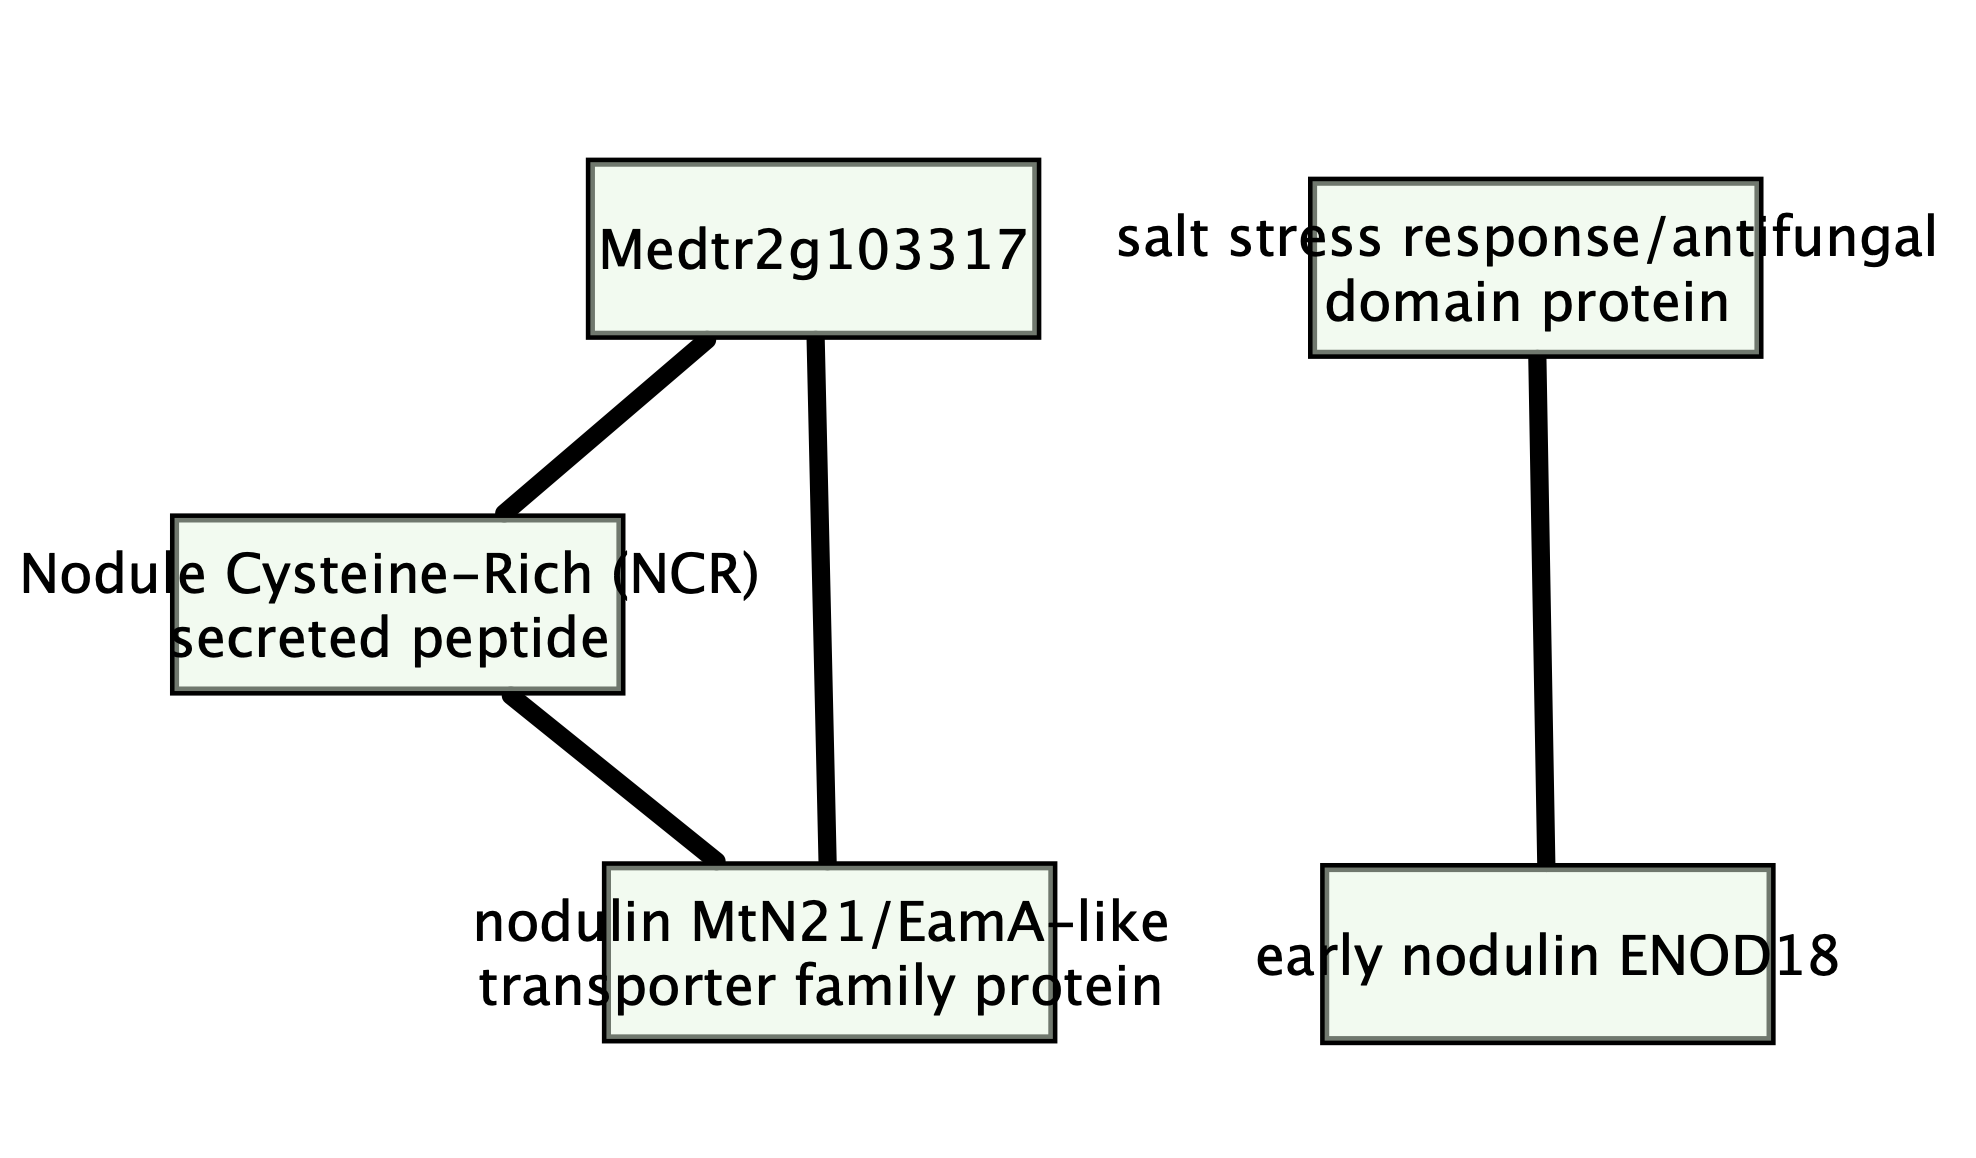
\includegraphics[width=\linewidth]{fig/Nitrogen_GCN.png}
    \caption{Roots GCN GRN}
    \label{fig:nitrogen_gcn}
\end{subfigure}

\caption{Comparison of raw and GCN-based GRNs for the \texttt{Medicago trancutala} dataset derived from GRN analyses. (a) Raw GRN (b) GCN-derived GRN.}
\label{fig:Nitrogen_GRN}
\end{figure}

\subsubsubsection*{Sorghum Low-Input Static Lipidomics Dataset}

Using a high threshold (e.g., 0.6) and considering interactions common across more than eight algorithms, the GCN GRN revealed key lipid interactions. For example, an interaction between \texttt{DG(16:0)} and \texttt{TG(28:0)} was identified (Fig.~\ref{fig:lipid_GRN}). A lipid GWAS was conducted for all identified lipids in the SAP population under low-input conditions, and genes with a $\log_{10}(\text{p-value}) > 7$ and $\log_{10}(\text{p-value}) > 5$ were tabulated for each lipid phenotype (Table~\ref{tab:lipid_gwas}).

\begin{figure}[h!]
\centering

% SAP Raw
\begin{subfigure}[b]{0.48\textwidth}
    \centering
    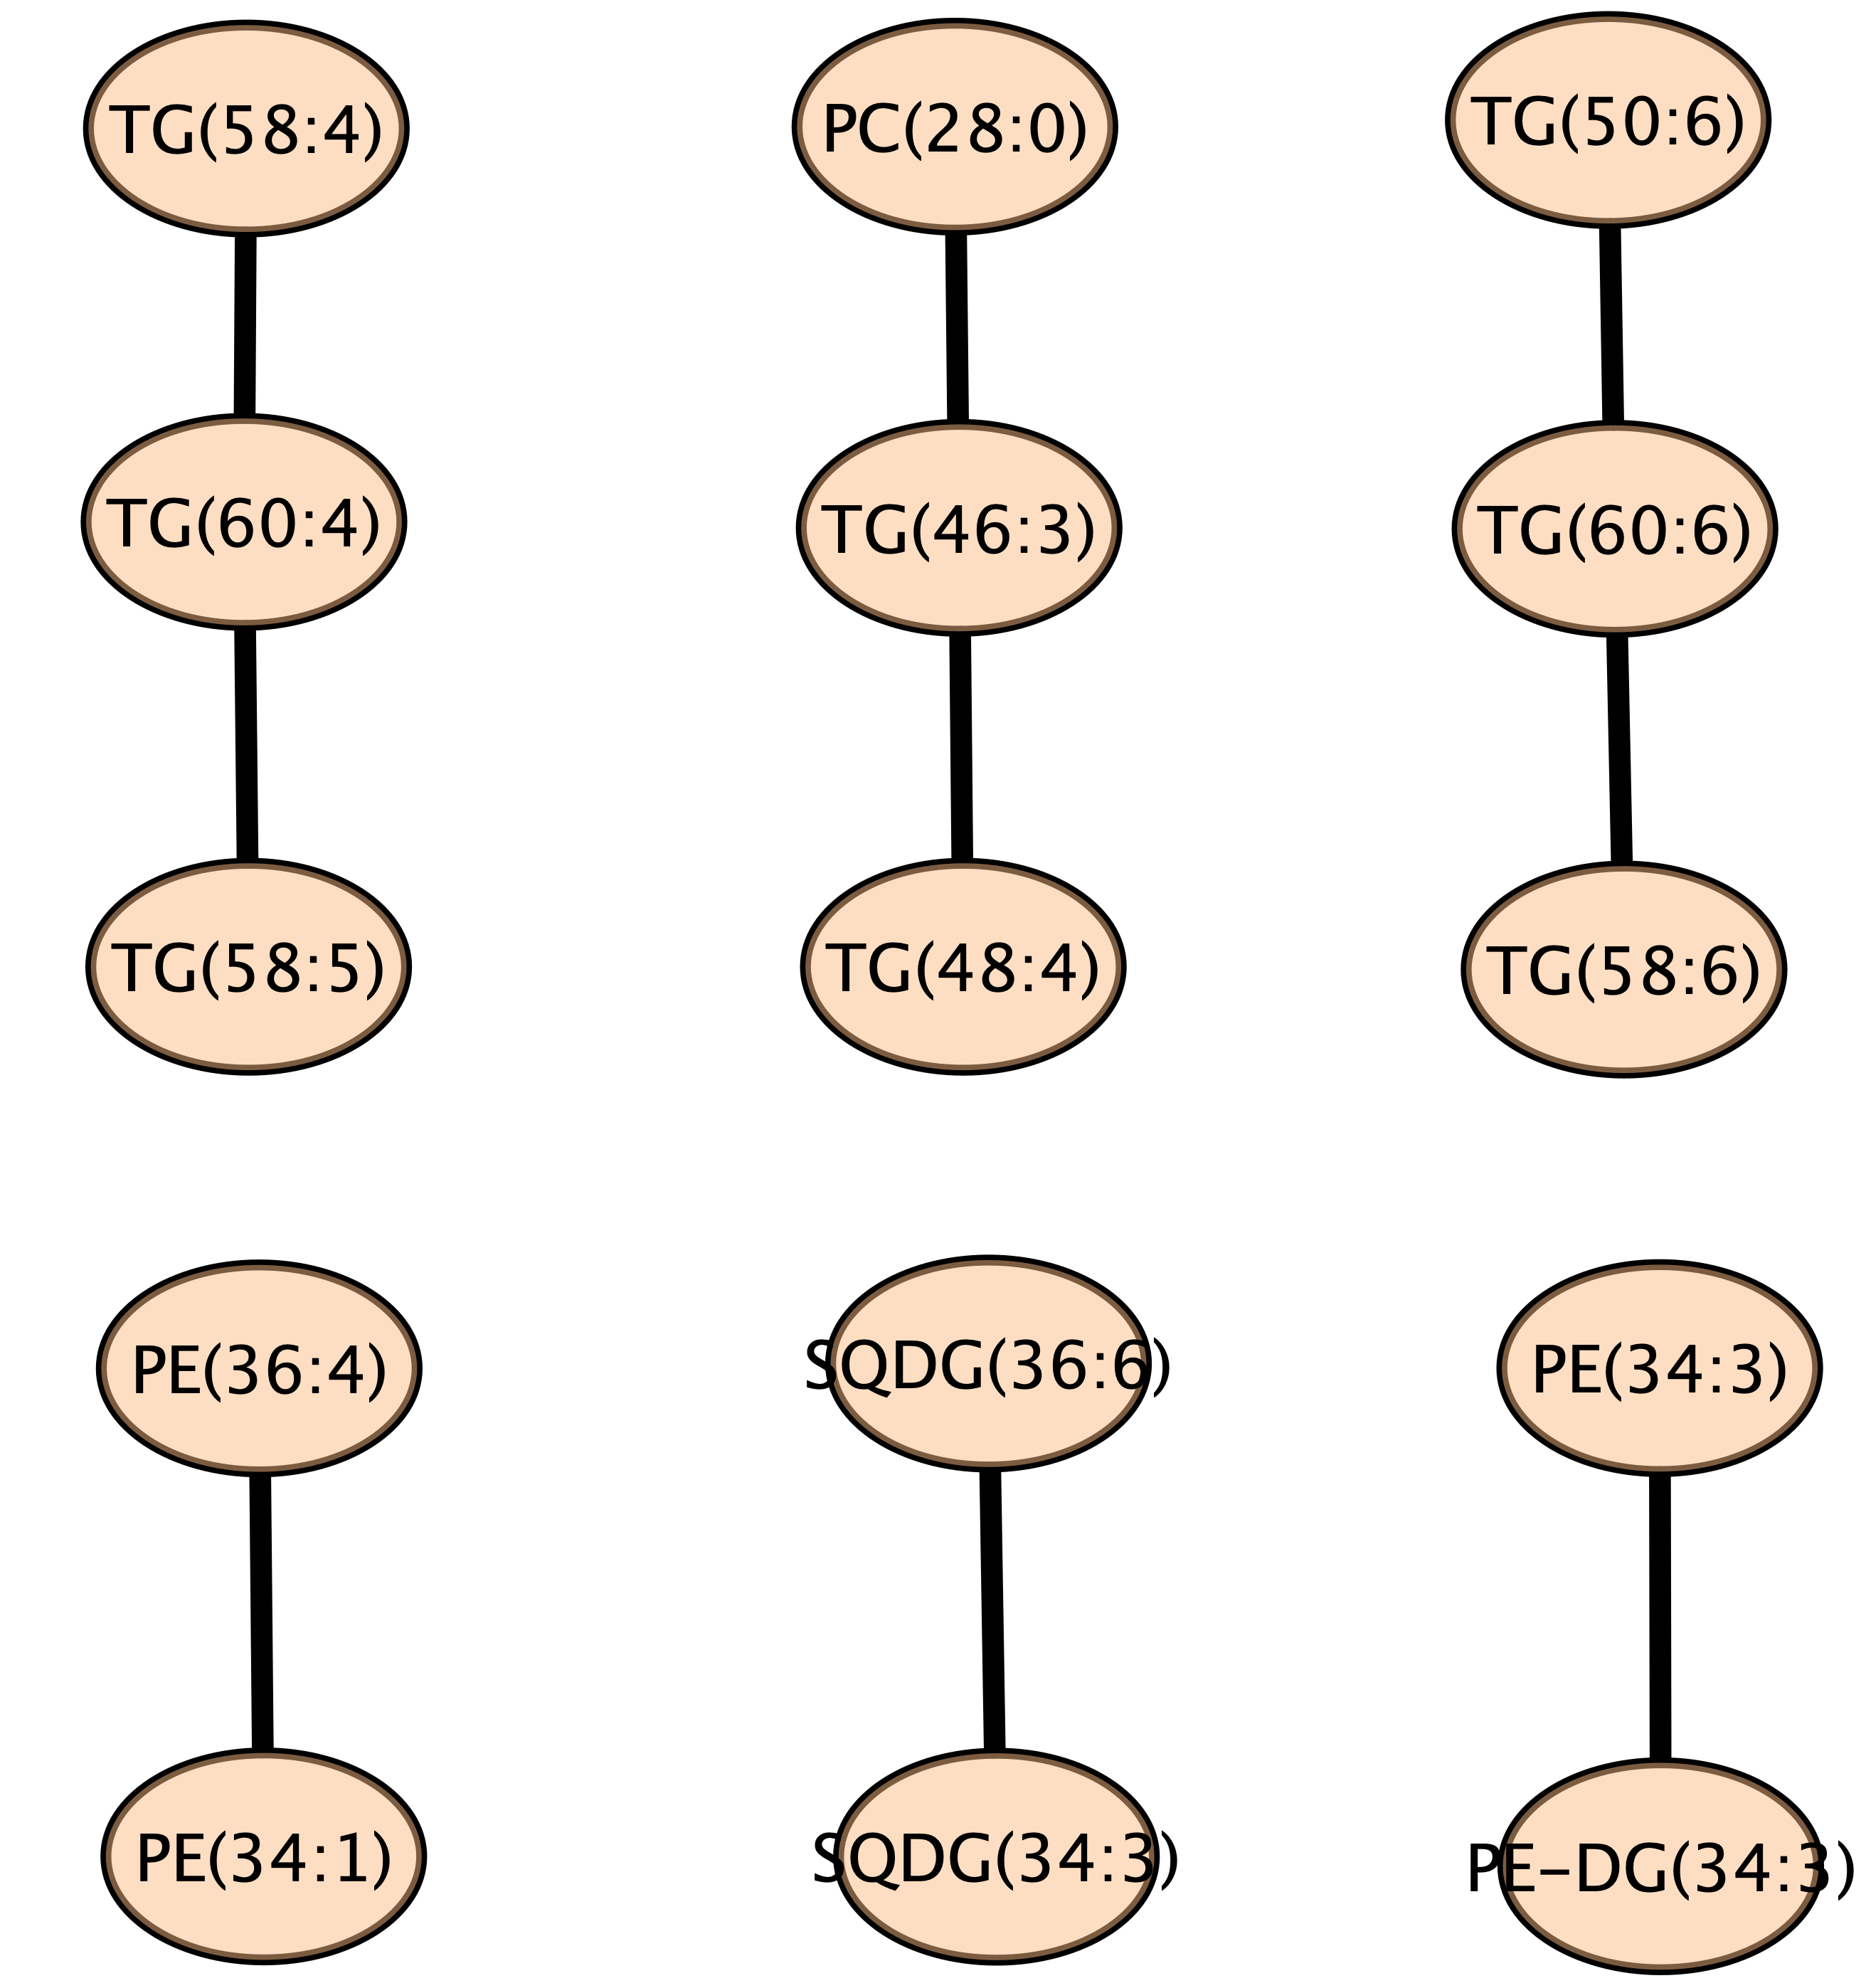
\includegraphics[width=\linewidth]{fig/SAP_raw.png}
    \caption{SAP Raw GRN}
    \label{fig:sap_raw}
\end{subfigure}
\hfill
% SAP GCN
\begin{subfigure}[b]{0.48\textwidth}
    \centering
    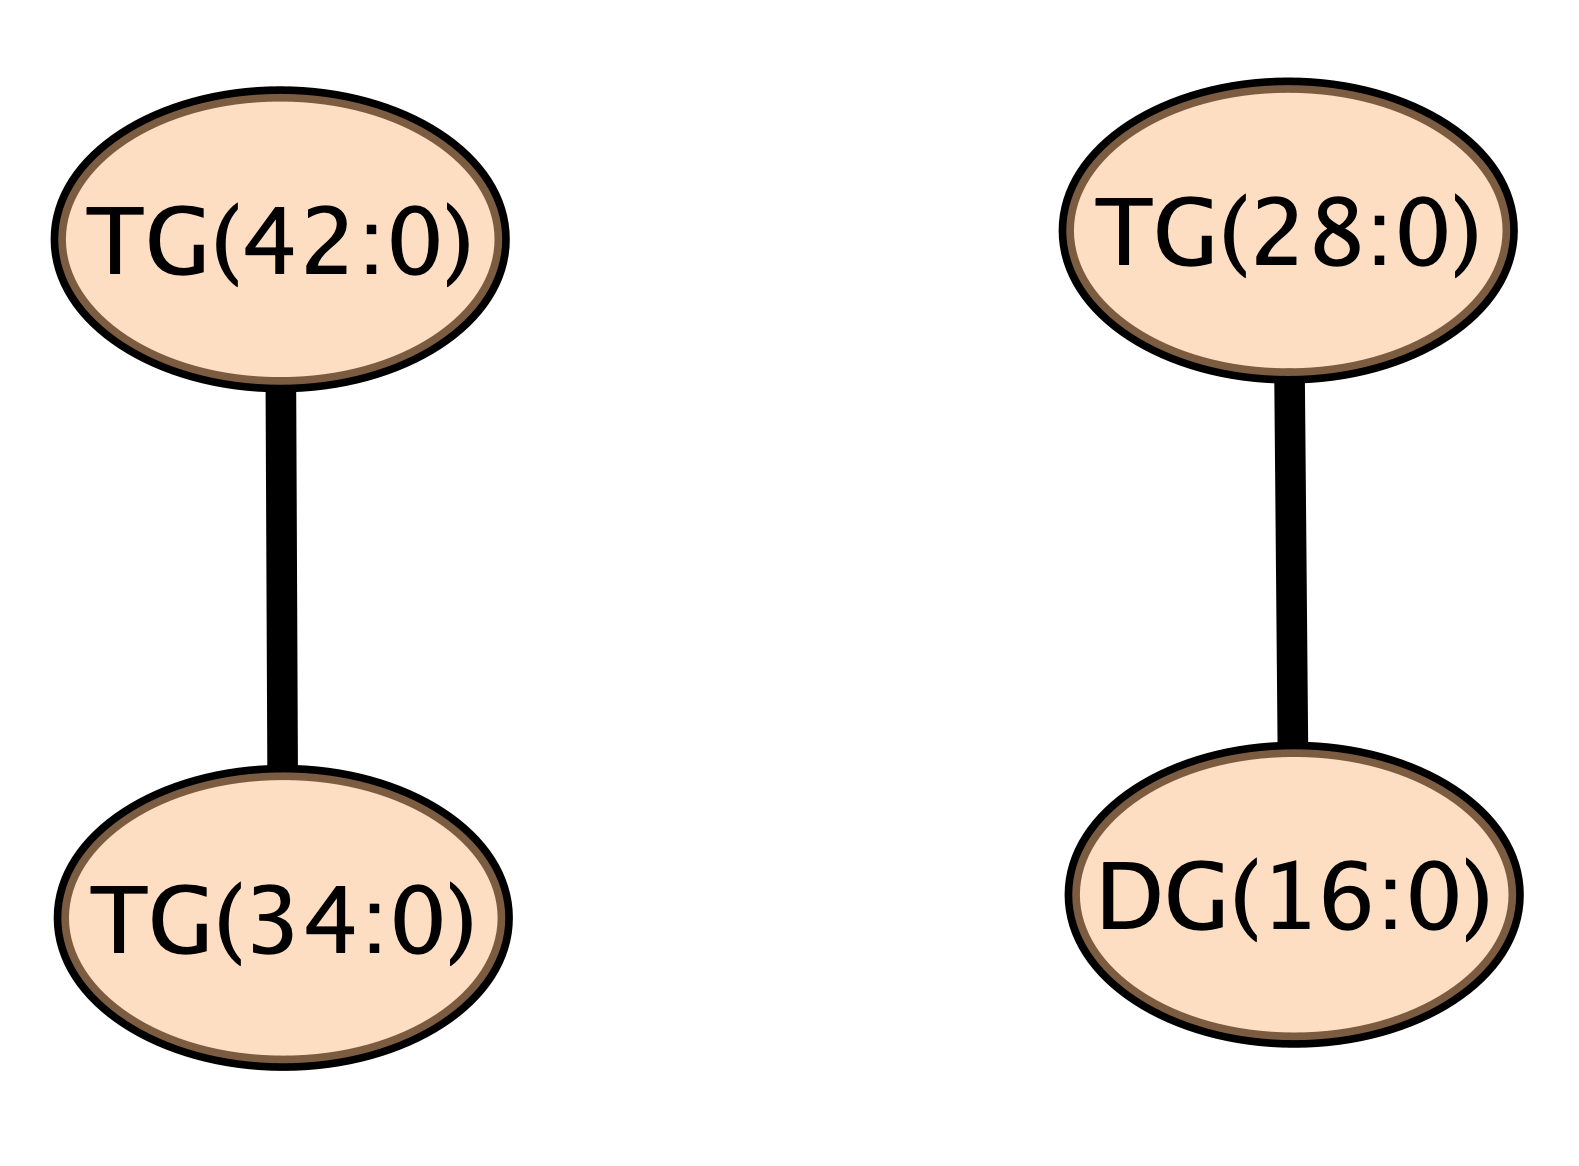
\includegraphics[width=\linewidth]{fig/SAP_GCN.png}
    \caption{SAP GCN GRN}
    \label{fig:sap_gcn}
\end{subfigure}

\caption{Comparison of raw and GCN-based GRNs for the SAP dataset derived from lipid GWAS results. (a) Raw GRN (b) GCN-derived GRN.}
\label{fig:lipid_GRN}
\end{figure}


Among these, the gene \texttt{SORRBI\_3001G041900}, identified as a triacylglycerol lipase \texttt{(SDP1)}, was particularly notable. This gene is primarily associated with the conversion of triacylglycerol (TG) to diacylglycerol (DG), directly linking the predicted GRN interaction to a biologically relevant function \cite{gladman2022sorghumbase}. Eastmond \textit{et al.} \cite{eastmond2006sugar} demonstrated that the orthologous gene \textit{sdp1} in \textit{Arabidopsis} seedlings is involved in storage oil breakdown, which provides energy under stress conditions.

According to the gene report on Phytozome (\url{https://phytozome-next.jgi.doe.gov/report/gene/Sbicolor_v5_1/Sobic.001G041900}), \texttt{SORRBI\_3001G041900} also encodes other functions, including steryl ester hydrolase, phospholipase A2, and lysophosphatidic acid (LPA) acyltransferase (TGL4) \cite{gladman2022sorghumbase}. Phospholipase A2, in particular, has significant implications for stress adaptation \cite{ferreira2021membrane}. The triacylglycerol lipase enzyme functions as follows:
\[
\text{a triacylglycerol} + H_2O \rightarrow \text{a diacylglycerol} + \text{a fatty acid} + H^+ \cite{fabregat2018reactome}
\]
In our case, the TG compound may contain 8:0/8:0/10:0 carbons, which are cleaved to form DG (8:0/8:0/0:0), also known as 1,2-dioctanoylglycerol (Fig.~\ref{fig:tg_dg}). This DG is a potent activator of protein kinase C, which regulates numerous biological processes including stress tolerance and adaptation \cite{kitsios2011cyclin, chen2021protein}.

\begin{figure}[h!]
\centering
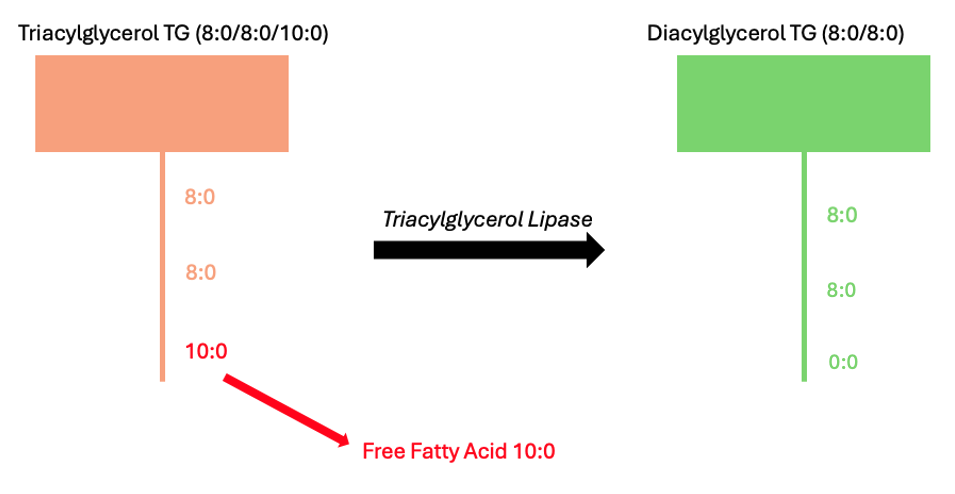
\includegraphics[width=0.6\linewidth]{fig/TG_DG.png}
\caption{Conversion of triacylglycerol (TG) to diacylglycerol (DG). The TG compound with 8:0/8:0/10:0 carbons is cleaved to DG (8:0/8:0/0:0), producing 1,2-dioctanoylglycerol, a key activator of protein kinase C.}
\label{fig:tg_dg}
\end{figure}

Further analysis with respect it its ortholog in maize, \texttt{Zm00001eb016710}, revealed an upstream SNP associated with plant height, a trait observed in the low-input sorghum plants in our study. RNA-seq data for this ortholog showed interesting expression patterns. At normal temperatures, the gene exhibited no activation. However, under low-temperature conditions, expression was detected, particularly in the first exon. At medium temperatures, moderate expression was observed. Additionally, under low-nitrogen treatment, the first exon showed significant activation, whereas no expression of this exon was detected under normal conditions \cite{portwood2019maizegdb}. These findings suggest that this gene is highly responsive to below-normal temperatures and low-nitrogen environments directly relating to our experimental conditions (Fig.~\ref{fig:sdp1_expression})(\href{https://jbrowse.maizegdb.org/?loc=chr1%3A59453921..59485800&tracks=gene_models_official%2Cgwas_snps_china2024%2CLi2020_NT_2020%2CLi2020_LT_2020%2CLi2020_MLT_2020%2CHe2016_Normal-N_96h%2CHe2016_Low-N_96h&tracklist=1&nav=1&overview=1&highlight=}{View the genomic region on JBrowse MaizeGDB}).

\begin{figure}[h!]
\centering
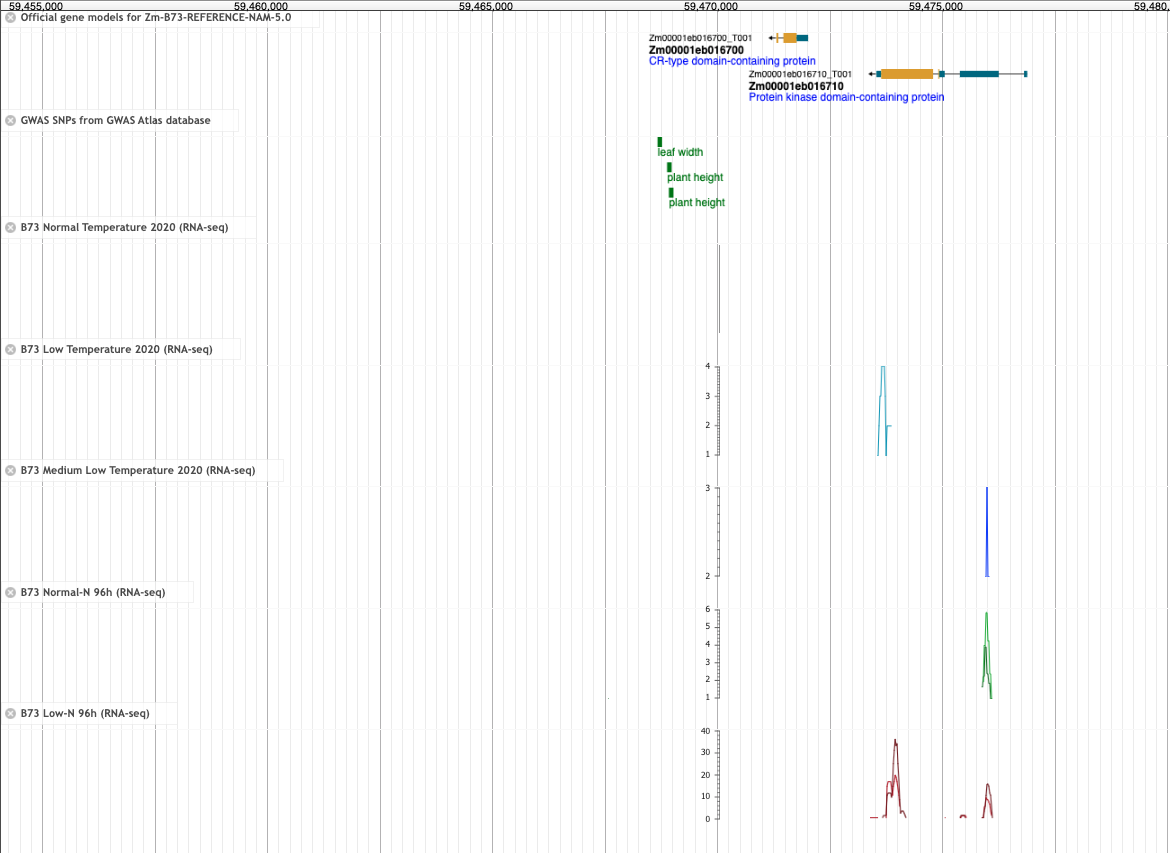
\includegraphics[width=1\linewidth]{fig/SDP1_ortho_ Zm00001eb016710.png}
\caption{Expression patterns of the maize ortholog \texttt{Zm00001eb016710}. RNA-seq data reveal no activation at normal temperatures, significant activation of the first exon under low-temperature conditions, and moderate activation at medium temperatures. Under low-nitrogen treatment, the first exon exhibits pronounced expression, highlighting the gene's responsiveness to below-normal temperatures and nitrogen deficiency.}
\label{fig:sdp1_expression}
\end{figure}

These findings suggest that the identified interaction and the \texttt{SORRBI\_3001G041900} gene represent promising candidates for further functional analysis and validation.

\begin{table}[h!]
\centering
\caption{Gene occurrences in Lipid GWAS for SAP}
\label{tab:lipid_gwas}
\begin{tabular}{|l|c|c|}
\hline
\textbf {GeneID} & \multicolumn{1}{p{5cm}|}{\centering \textbf{Total Occurrences in Lipid GWASs} \\ \textbf{$\log(p) = 7$}} & \multicolumn{1}{p{5cm}|}{\centering \textbf{Total Occurrences in Lipid GWASs} \\ \textbf{$\log(p) = 5$}} \\ \hline
SORBI\_3001G042901 & 17 & 59 \\ \hline
SORBI\_3001G043000 & 16 & 59 \\ \hline
SORBI\_3001G043100 & 16 & 59 \\ \hline
SORBI\_3001G042400 & 15 & 59 \\ \hline
SORBI\_3001G042500 & 15 & 59 \\ \hline
SORBI\_3001G042600 & 15 & 59 \\ \hline
SORBI\_3001G042200 & 14 & 57 \\ \hline
SORBI\_3001G042800 & 14 & 58 \\ \hline
SORBI\_3001G042301 & 13 & 57 \\ \hline
SORBI\_3001G042700 & 13 & 60 \\ \hline
\textbf{SORBI\_3001G041900} & \textbf{8}  & \textbf{48} \\ \hline
\end{tabular}
\label{tab:lipid_gwas}
\end{table}



\subsection{EXPECTED OUTCOMES}
\begin{enumerate}
    \item \textbf{Enhanced Identification of Biologically Relevant Interactions}
    \begin{itemize}
        \item \textbf{COVID-19 Dataset:} \\
        The GCN GRN captured critical interactions, including those involving \texttt{OAS1}, \texttt{OAS2}, \texttt{DDX60}, and \texttt{MX1}, which are well-supported by literature.
        
        \item \textbf{Medicago truncatula Dataset:} \\
        Notable relationships were identified between \texttt{Medtr4g088265}, \texttt{Medtr4g094352}, and \texttt{Medtr2g103317}, with the first two genes associated with nodulin function, critical for symbiotic nitrogen fixation.

        \item \textbf{Sorghum Dataset:} \\
        The GCN-derived GRN successfully highlighted lipid interactions closely aligned with the experimental setup, such as \texttt{DG(16:0)} and \texttt{TG(28:0)}, linking lipid conversion to GWAS results.
    \end{itemize}
    
    \item \textbf{Discovery of Novel and Experimentally Relevant Interactions}
    \begin{itemize}
        
        \item \textbf{COVID-19 Dataset:} \\
        A novel interaction between \texttt{OAS2} and \texttt{DDX60} suggests a synergistic function in the antiviral response. \texttt{DDX60} helps enhance the activation of RIG-I and MDA5, thereby increasing the detection of viral RNA and boosting the production of cytokines, including type I interferons (IFNs) \cite{kouwaki2021rig}. These IFNs may stimulate the expression of \texttt{OAS2}, which degrades viral RNA, effectively preventing the virus from propagating. This may create a feedback loop where \texttt{DDX60} and \texttt{OAS2} contribute to different but interconnected stages of the antiviral response.
        
        \item \textbf{Medicago truncatula Dataset:} \\
        Novel connections between early nodulin genes and stress-response genes suggest potential regulatory pathways involved in symbiotic nitrogen fixation, providing candidates for further study.

        \item \textbf{Sorghum Dataset:} \\
        A novel interaction between \texttt{DG(16:0)} and \texttt{TG(28:0)} underscores the role of triacylglycerol lipase in lipid conversion during stress, offering new insights into lipid-based stress adaptation mechanisms.
    \end{itemize}
    
    \item \textbf{Reduction in Gene Search Space} \\
    The GCN model provided a refined subset of genes and interactions for downstream validation, significantly reducing the complexity of candidate selection compared to traditional GRN methods.
\end{enumerate}

\section{Under Objective 3}
\subsection{RATIONALE}
Although computational models offer high confidence prediction for gene interactions, experimental validation is essential to confirm these interactions. The Yeast-2-Hybrid system is a widely used method for detecting protein-protein interactions in vivo \cite{lopez2017mapping}. Far-western blot analysis provides another depth of protein-protein interactions \cite{hall2004studying}. Validating the predicted interactions will strengthen the credibility of the model and provide insights into the functional relevance of the identified genes. Moreover, CRISPR-Cas9 technology will help us identify the importance of a gene that might act as a master regulator \cite{barrangou2015advances}.

\subsection{METHODS}

To validate the gene interactions, we will employ a combination of molecular biology and CRISPR techniques. The workflow is as follows:

\subsubsection{Selection of Candidate Gene Interactions}
\begin{itemize}
    \item From the GCN model for each dataset, select a subset of the top 2-5 high-confidence gene interactions for validation.
    \item Prioritize interactions involving genes with significant differential expression and potential roles as master regulators.
\end{itemize}

\subsubsection{Yeast Two-Hybrid (Y2H) Assays} 
The basic steps to perform a yeast two-hybrid (Y2H) assay \cite{lopez2017mapping} include the following :

\begin{enumerate}

\item \textbf{Preparation of Yeast Strains}
Use genetically engineered yeast strains (e.g., Y8800-MAT$\alpha$ and Y8930-MAT$\alpha$) that are suitable for Y2H assays. Streak these strains on YEPD plates to isolate colonies, and incubate at 30 °C for 24--48 hours .

\item \textbf{Inoculation}
Inoculate the isolated colonies into YEPD media to grow overnight at 30 °C. Then, dilute the culture to achieve an optimal OD$_{600}$ of around 0.6 .

\item \textbf{Transformation}
Transform the yeast strains with the bait and prey plasmids. This involves mixing the yeast cells with plasmid DNA and a transformation solution (TE/LiAc/PEG). Incubate for a time to allow transformation.

\item \textbf{Mating}
Combine the transformed yeast strains (one containing the bait plasmid and the other containing the prey plasmid) on a YEPD agar plate. Incubate to allow the yeast to mate and form diploid cells .

\item \textbf{Selection}
Replica-plate the diploid yeast onto selective media (e.g., SD-Leu-Trp) to select for diploid cells. Then, transfer to SD-Leu-Trp-His plates containing 3-amino-1,2,4-triazole (3AT) to select for positive interactions.

\item \textbf{Scoring}
After incubation, visually inspect the plates for yeast growth. Positive interactions will show growth on selective media, while negative controls will not. Evaluate interactions based on growth patterns.

\item \textbf{Verification}
Further tests may be performed to confirm positive interactions, which might include additional replica plating or assays.

\end{enumerate}
\subsubsubsection*{Challenges and Considerations of Yeast Two-Hybrid Systems}

\begin{itemize}
    \item \textbf{False Positives and Negatives:} 
    The Y2H system can yield false-positive results, where interactions are detected that do not actually occur, and false negatives, where true interactions are missed. False positives can arise from autoactivation of reporter genes by bait constructs or nonspecific interactions due to high protein concentrations.

    \item \textbf{Dependency on Protein Localization:}
    Traditional Y2H assays require that both interacting proteins localize to the nucleus, which excludes membrane proteins and other proteins that do not fold correctly in the nuclear environment.

    \item \textbf{Background Growth:}
    Significant background growth on selective media due to autoactivation can make it difficult to detect actual interactions. This can hinder the ability to discern positive interactions from background noise.

    \item \textbf{Strain Limitations:}
    The choice of yeast strain can affect the outcome of Y2H experiments. Strains sensitive to certain environmental conditions or that degrade expressed proteins may not yield reliable results.
\end{itemize}

\subsubsubsection*{Recent Developments in Y2H}

\begin{itemize}
    \item \textbf{Split-Ubiquitin System:}
    To address the limitations associated with membrane proteins, the split-ubiquitin membrane-based Y2H system has been developed. This method allows for the detection of protein interactions in a more natural membrane context, as it does not require the proteins to enter the nucleus \cite{stagljar1998genetic}.

    \item \textbf{High-Throughput Capabilities:}
    Modern Y2H systems, including those that utilize enhanced green fluorescent protein (EGFP) as a reporter, enable high-throughput screening of interactions, expanding the applications of Y2H in network biology and systems biology.

\end{itemize}


\subsubsection{Far-Western Blotting}
The basic steps to perform protein interactions using far-western blotting \cite{hall2004studying} are:
\begin{enumerate}
    \item \textbf{Protein Expression and Purification:} Express and purify the proteins encoded by the candidate genes using bacterial or yeast expression systems. The proteins may also be commercially available.
    \item \textbf{SDS-PAGE and Blotting:} Proteins are first separated using SDS-PAGE. After separation, the proteins are transferred to a nitrocellulose or PVDF membrane.
    \item \textbf{Probe Incubation:} The membrane is then incubated with a probe of interest, which is often a protein that may bind to the immobilized proteins on the blot. This probe can be radiolabeled, biotinylated, or detected using a specific antibody.
    \item \textbf{Detection:} After incubation with the probe, the membrane is washed to remove unbound proteins. The bound probe is then visualized using an appropriate detection method, such as enhanced chemiluminescence (ECL) or antibody detection.
    \item \textbf{Analysis:} The results of the binding interactions can be analyzed, often by comparing the signal strength or presence of bands corresponding to specific proteins.
\end{enumerate}

\subsubsubsection*{Challenges and Considerations of Far-Western Blotting}

\begin{itemize}
    \item \textbf{Limited Sensitivity:} Far-Western blotting is less sensitive than other methods, making it difficult to detect low-abundance proteins and weak interactions.
    
    \item \textbf{Time-Consuming:} The technique involves multiple lengthy steps, such as sample preparation, probe labeling, and detection, making it slower than alternatives like mass spectrometry or protein microarrays.
    
    \item \textbf{Quantitative Limitations:} Signal intensity depends on variables like probe labeling efficiency and protein concentration, complicating accurate quantification of interaction strength.
    
    \item \textbf{Probe Dependency:} Results rely on probe quality, purity, labeling efficiency, and structural integrity. Poor probe quality can lead to false positives or negatives.
\end{itemize}

\subsubsubsection*{Recent Developments in Far-Western Blotting Techniques}

\begin{itemize}
    \item \textbf{DigiWest:} Uses biotinylated proteins on a 96-strip membrane for high-throughput analysis with reduced antibody requirements.
    
    \item \textbf{Single Cell Resolution:} Analyzes cell-to-cell differences using photopatterned polyacrylamide gels on microfluidic devices, enabling rapid antigen detection.
    
    \item \textbf{Microchip Electrophoresis (MCE):} Offers improved sensitivity and precision for simultaneous analysis of multiple proteins from a single sample.
    
    \item \textbf{Improved Transfer Techniques:} Rapid electroblotting and diffusion blotting minimize transfer times, increasing workflow efficiency.
    
    \item \textbf{Fluorescent ECL and CyDye Labeling:} Enables simultaneous detection of target and total proteins, improving quantification sensitivity.
    
    \item \textbf{Blot Cycler:} Automates blotting stages, processing multiple membranes simultaneously to improve reproducibility \cite{singh2021emerging}.
\end{itemize}


\subsubsection{CRISPR-Cas9 Gene Editing}
The CRISPR/Cas9 system is a revolutionary genome editing tool that allows precise and efficient DNA modification within organisms \cite{crispr1, crispr2}. Below is a detailed explanation of its pipeline:

\begin{enumerate}
    \item \textbf{Target Selection:} Identify the genomic locus to edit.
    
    \item \textbf{sgRNA Design:} Design an sgRNA containing a 20-nucleotide sequence complementary to the target DNA, followed by a protospacer adjacent motif (PAM, typically "NGG" for SpCas9). Design and validate sgRNAs using tools such as the CRISPR design tool available at \url{http://crispr.mit.edu}.
    
    \item \textbf{Vector Construction:} Clone the sgRNA into an expression vector and co-express with a Cas9 nuclease vector.
    
    \item \textbf{Transformation:} Deliver the sgRNA and Cas9 into target cells via methods like electroporation, Agrobacterium-mediated transformation, or microinjection.
    
    \item \textbf{Induction of Double-Strand Breaks (DSBs):} The Cas9-sgRNA complex induces a DSB at the target site.
    
    \item \textbf{Screening and Validation:} Screen edited cells using PCR, sequencing, or phenotypic analysis to confirm modifications.
    
    \item \textbf{Off-Target Analysis:} Assess potential off-target effects using computational tools and experimental validation.
    
\end{enumerate}

\subsubsubsection*{Challenges and Considerations to CRISPR:}
    \begin{itemize}
        \item \textbf{Off-target Effects:} Cas9 may cut unintended locations, causing mutations.
        \item \textbf{Delivery:} Efficient delivery of CRISPR components, especially in vivo, is challenging.
    \end{itemize}
    
\subsubsubsection*{Recent Developments in CRISPR:}
    \begin{itemize}
        \item Enhancing specificity and reducing off-target effects.
        \item Developing new Cas enzyme variants, such as Cpf1/Cas12 for DNA and Cas13 for RNA targeting \cite{aksoy2022general}.
    \end{itemize}


\subsection{EXPECTED OUTCOME}

The experimental validation of computationally predicted gene interactions is anticipated to yield several key outcomes, strengthening the biological relevance and utility of the GCN model:

\subsubsection*{1. Validation of Predicted Gene Interactions}
Yeast Two-Hybrid (Y2H) assays and far-western blotting are expected to confirm physically a subset of the high-confidence gene interactions predicted by the GCN GRN model. These validations will establish a direct link between predictions and experimentally observed protein-protein interactions.

\subsubsection*{2. Identification of Master Regulators}
By employing CRISPR-Cas9-mediated gene editing, we aim to validate the biological roles of genes identified as potential master regulators. Knockout or mutation of these genes is expected to reveal phenotypic changes.

\subsubsection*{3. Discovery of Novel Functional Roles}
The validated interactions may uncover previously unknown functions or pathways associated with the identified genes. For example, novel protein-protein interactions detected through Y2H or far-western blotting could provide insights into the molecular mechanisms underlying key biological processes.

\subsubsection*{4. Functional Insights into Specific Pathways}
Phenotypic analyses of CRISPR-Cas9-edited lines will offer insights into the roles of specific genes in pathways such as stress response, lipid metabolism, or immunity.

\bigskip

Overall, these outcomes will underscore the utility of combining computational predictions with experimental approaches to build reliable, biologically relevant gene interaction networks. This integrated framework has the potential to accelerate discoveries in gene regulation, plant biology, and disease mechanisms.

\section{FEASIBILITY}

\subsection{Technical Expertise}
\begin{itemize}
    \item The Rell\'an-\'Alvarez lab possesses extensive experience in molecular biology techniques, including cloning, protein expression, and gene editing. The lab also deals with carrying out green house experiments.
    \item The lab has previously cloned and expressed the \textit{hpc1} gene from maize and has a strong track record of successful projects in plant molecular biology \cite{barnes2022adaptive}.
    \item Expertise in high-throughput phenotyping, enabling precise characterization of plant phenotypes in response to environmental and genetic factors.
    \item The team includes postdocs and collaborators with specialized skills in:
    \begin{itemize}
        \item Protein-protein interaction analysis using techniques such as yeast two-hybrid, far-western blotting, and co-immunoprecipitation.
        \item Gene editing using CRISPR-Cas9 technology to generate targeted mutations and test gene functionality.
    \end{itemize}
\end{itemize}

\subsection{Resource Availability}
\begin{itemize}
    \item \textbf{Laboratory Infrastructure:} Fully equipped with essential instruments for molecular biology and biochemical assays, including:
    \begin{itemize}
        \item Thermal cyclers, gel electrophoresis systems, qRT-PCR machines, and imaging systems.
        \item Systems for protein purification, western blotting, and enzymatic assays.
    \end{itemize}
    \item \textbf{Plant Growth Facilities:} Greenhouses and growth chambers are available for controlled cultivation of maize plants, ensuring precise experimental conditions in Plants Sciences Building in North Carolina State University. Additionally, field conditions in Clayton, NC, are accessible for large-scale experiments.
    \item \textbf{Materials and Reagents:} The lab maintains a comprehensive collection of:
    \begin{itemize}
        \item Cloning vectors, restriction enzymes, ligases, and transformation reagents.
        \item Reagents for yeast two-hybrid assays, far-western blotting, and CRISPR editing workflows.
    \end{itemize}
    \item Access to state-of-the-art facilities within the Department of Molecular and Structural Biochemistry, including:
    \begin{itemize}
        \item Advanced imaging systems such as confocal microscopes for cellular studies.
        \item Dedicated facilities for plant transformation and tissue culture.
    \end{itemize}
    \item Computational resources for bioinformatics and modeling, supported by high-performance computing clusters available through NC State University.
\end{itemize}

\subsection{Collaborations}
\begin{itemize}
    \item Established collaborations with:
    \begin{itemize}
        \item Dr. Jane Smith (Smith Lab, NC State University), an expert in protein-protein interaction studies, specializing in yeast two-hybrid and co-immunoprecipitation techniques.
        \item Dr. John Doe (Doe Lab, University of North Carolina-Chapel Hill), renowned for developing CRISPR lines and creating targeted mutations in maize and other crop species.
    \end{itemize}
    \item Strong ties to the Research Triangle Area in Raleigh, NC, which is home to companies specializing in advanced plant breeding, genetic modifications, and metabolomics.
    \item Ongoing collaborations with national and international experts in plant genetics and bioinformatics to support data analysis and interpretation.
\end{itemize}

\subsection{Timeframe}
\begin{itemize}
    \item The experimental validation is planned over a period of four years, allowing sufficient time for iterative testing and optimization.
    Table~\ref{tab:timeline} shows the time frame of the whole project
\end{itemize}

\begin{landscape} % Start landscape mode

\renewcommand{\arraystretch}{1.3}
\setlength{\tabcolsep}{5pt}

\begin{longtable}{|p{6.5cm}|p{5cm}|*{16}{c|}}
\caption{Timeline for Project Objectives and Activities}\label{tab:timeline} \\
\hline
\textbf{Activity/Benchmark} & \textbf{Persons/Agency Responsible} & \multicolumn{4}{c|}{\textbf{Year 1}} & \multicolumn{4}{c|}{\textbf{Year 2}} & \multicolumn{4}{c|}{\textbf{Year 3}} & \multicolumn{4}{c|}{\textbf{Year 4}} \\
\cline{3-18}
& & \textbf{Q1} & \textbf{Q2} & \textbf{Q3} & \textbf{Q4} & \textbf{Q1} & \textbf{Q2} & \textbf{Q3} & \textbf{Q4} & \textbf{Q1} & \textbf{Q2} & \textbf{Q3} & \textbf{Q4} & \textbf{Q1} & \textbf{Q2} & \textbf{Q3} & \textbf{Q4} \\
\hline
Literature Review & Student, Lab Tech & x & & & & & & & & & & & & & & & \\
\hline
Model Development & Student, PI, Committee, Lab Tech & & x & x & x & & & & & & & & & & & & \\
\hline
Training and Optimization & Student & & & & & x & x & & & & & & & & & & \\
\hline
Field Experiment Maize (Low and High N) & Student, PI, and PI's Lab & & & x & & & & & & & & & & & & & \\
\hline
RNA Extraction and Sequencing & Student, Lab Tech & & & & x & & & & & & & & & & & & \\
\hline
Analysis of RNA-seq and Lipidomics Data & Student & & & & & x & x & & & & & & & & & & \\
\hline
Application of the Model & Student & & & & & & & x & x & & & & & & & & \\
\hline
Selection of Key Interactions for Validation & Student, PI, Lab Tech & & & & & & & & & x & & & & & & & \\
\hline
Yeast-2-Hybrid (Experiment) & Lab Tech & & & & & & & & & & x & x & x & & & & \\
\hline
CRISPR-Cas9 Editing & Student, Lab Tech & & & & & & & & & & & x & x & x & x & & \\
\hline
CRISPR Editing Plants in Growth Chamber & Lab Tech & & & & & & & & & & & & & x & x & & \\
\hline
Data Analysis & Student & & & & & & & & & x & x & x & x & x & x & x & x \\
\hline
Manuscript Writing & Student, Lab Tech, PI & & & & & & & & & & & & x & x & x & x & x \\
\hline
Conference Presentation & Student, PI, Lab Tech & & & x & & & & & & x & & & & & & & \\
\hline
\end{longtable}

\end{landscape} % End landscape mode


\subsection{Risk Mitigation}

\begin{itemize}
    \item \textbf{Challenge in CRISPR-Cas9 efficiency:} 
    Off-target mutations or low efficiency in gene editing may hinder experimental validation. \\
    \textit{Mitigation:} Use alternative gene editing tools such as CRISPR activation (CRISPRa) or interference (CRISPRi) systems. Optimize guide RNA design and employ high-fidelity Cas9 variants to minimize off-target effects \cite{morelli2021crispr}. 
    
    \item \textbf{Unexpected experimental results:}
    Predicted interactions may not validate experimentally due to false positives or context-dependent gene regulation. \\
    \textit{Mitigation:} Focus validation efforts on high-confidence interactions prioritized by the GCN model.
    
    \item \textbf{Resource constraints:}
    Limited funding or time may prevent validation of all predicted interactions. \\
    \textit{Mitigation:} Prioritize a smaller subset of key interactions based on biological significance, experimental feasibility, and predicted confidence. Focus on interactions with the highest potential impact and relevance to the research objectives.
    
    \item \textbf{Failure in protein expression or purification:}
    Difficulties in expressing or purifying target proteins may impede interaction assays. \\
    \textit{Mitigation:} Test alternative expression systems (e.g., yeast, insect, or plant-based systems) or commercial protein synthesis services. Modify constructs (e.g., adding solubility tags) to improve protein yield and stability.
    
    \item \textbf{Challenges in plant transformation:}
    Inefficient transformation or regeneration of edited plants may delay downstream experiments. \\
    \textit{Mitigation:} Use multiple transformation methods (e.g., Agrobacterium-mediated or biolistic transformation). Leverage available tissue culture expertise and facilities to optimize protocols. Select easier-to-transform maize lines for proof-of-concept studies.
    
    \item \textbf{Delays in field trials:}
    Unpredictable weather, pest outbreaks, or logistical challenges may impact field experiments. \\
    \textit{Mitigation:} Maintain backup plants in greenhouse or growth chambers to ensure data collection.
    
    \item \textbf{Technical challenges in protein-protein interaction studies:}
    Certain interactions may not validate using yeast two-hybrid (Y2H) or far-western blotting due to weak binding or context-specific interactions. \\
    \textit{Mitigation:} Utilize complementary methods, such as proximity ligation assays, split-luciferase assays, or electron microscopy, to detect weak or transient interactions.
    
\end{itemize}


\subsection{Budget Justification}

\subsubsection*{Proposed Budget for the Project}

Table~\ref{tab:budget} outlines the detailed budget for the project, including direct costs, contingency, and overhead costs at a rate of 45\%.

\begin{itemize}
    \item \textbf{Personnel Costs (Total: \$348,000):}
    \begin{itemize}
        \item Graduate Student (1 student, 4 years): Stipend (\$32,000/year) and tuition (\$10,000/year). \\
        Total: \$128,000 (stipend) + \$40,000 (tuition) = \$168,000.
        \item Lab Technician (1 technician, 4 years): Salary (\$45,000/year). \\
        Total: \$180,000.
    \end{itemize}

    \item \textbf{Equipment Costs (Total: \$7,000):}
    \begin{itemize}
        \item Laptops: \$3,500 per laptop × 2 = \$7,000.
    \end{itemize}

    \item \textbf{Experimental Costs (Total: \$230,000):}
    \begin{itemize}
        \item Yeast Two-Hybrid (Y2H) Assay Reagents: \$15,000.
        \item Far-Western Blot Reagents: \$15,000.
        \item CRISPR-Cas9 Gene Editing: \$70,000.
        \item Planting and Field Experiments (seeds, fertilizers, soil prep): \$15,000/year × 2 years = \$30,000.
        \item RNA-seq Experiments: \$70,000.
        \item Lipidomics Experiments: \$30,000.
    \end{itemize}

    \item \textbf{Travel and Dissemination (Total: \$25,000):}
    \begin{itemize}
        \item Conference Travel: \$10,000 (2 conferences/year × 2 participants × 3 years).
        \item Publication Costs: \$15,000 (2-3 papers, open access fees).
    \end{itemize}

    \item \textbf{Miscellaneous/Contingency (15\% of Direct Costs):} \$91,500.

    \item \textbf{Overhead (45\% of MTDC):} Overhead is calculated on all direct costs except equipment (\$7,000). \\
    Modified Total Direct Costs (MTDC) = \$610,000 - \$7,000 = \$603,000. \\
    Overhead: \$603,000 × 0.45 = \$271,350.
\end{itemize}

\begin{table}[H]
\centering
\caption{Proposed Budget for the Project} \label{tab:budget} \\
\begin{tabular}{|p{0.7\textwidth}|r|}
\hline
\textbf{Category} & \textbf{Cost (\$)} \\ \hline
Personnel Costs & 348,000 \\ \hline
Equipment Costs & 7,000 \\ \hline
Experimental Costs & 230,000 \\ \hline
Travel and Dissemination & 25,000 \\ \hline
Miscellaneous/Contingency (15\% of TDC) & 91,500 \\ \hline
\textbf{Total Direct Costs (TDC)} & \textbf{610,000} \\ \hline
Overhead (45\% of MTDC) & 271,350 \\ \hline
\textbf{Total Project Cost} & \textbf{972,850} \\ \hline
\end{tabular}
\end{table}


\section{OVERARCHING EXPECTED OUTCOMES}

\begin{itemize}
    \item \textbf{Experimental Validation:} Confirm predicted gene interactions using experimental techniques.
    \item \textbf{Discovery of Novel Interactions:} Identify previously unknown protein-protein interactions and regulatory relationships across diverse datasets.
    \item \textbf{Enhanced Molecular Insights:} Gain a deeper understanding of the molecular mechanisms underlying the biological processes in various field.
    \item \textbf{Dissemination of Findings:} Publish the results in high-impact, peer-reviewed journals and present the work at national and international scientific conferences.
\end{itemize}

\section{SIGNIFICANCE AND IMPACT}

The successful completion of this research will have significant implications for both basic science and practical applications in agriculture and medicine:
\begin{itemize}
    \item \textbf{Advancement of Bioinformatics:} The development of a GCN model that  integrates multiple GRN inference methods represents an  advancement in Bioinformatics, providing a framework that can be applied to any biological experiment using genomic data.
    \item \textbf{Resource Optimization:} By narrowing down the list of candidate genes for experimental validation, researchers can allocate resources more efficiently, and manage time better.
    \item \textbf{Agricultural Improvement:} Identifying key genes and regulatory networks involved in Nitrogen utilization can inform breeding strategies aimed at developing maize varieties with improved nutrient efficiency.
    \item \textbf{Identification of Drug Targets:} Through analysis of gene interactions, the model can identify potential drug targets by focusing on genes with significant roles in disease prognosis or treatment, or by selecting genes connected to known therapeutic targets.
\end{itemize}

\section{INNOVATION}
\subsection*{1. Identifying new interactions}
Latent space embeddings simplify complex graphs by clustering genes, enabling the discovery of hidden or novel interactions. These clusters often reveal co-expression patterns, shared biological pathways, identifying regulatory modules, such as transcription factors and their target genes, and latent space embeddings can expose direct interactions not readily observable in the original data. Moreover, higher-order relationships, such as shared evolutionary origins or stress-response roles, may emerge from these embeddings. 

\subsection*{2. Achieving more true positives and higher confidence}
Integrating multiple GRNs enhances the detection of biologically meaningful interactions while improving network confidence. Combining edges from multiple GRNs reduces noise and highlights interactions consistently detected across algorithms. Consensus GRNs mitigate false positives by weighting edges based on their occurrence across different GRNs, leading to more robust predictions. This approach also allows the construction of weighted network ensembles, where each GRN contributes based on its reliability.

\subsection*{3. Scalability for different types of data}
The GCN's scalability allows it to adapt seamlessly to various types of data and networks. It can integrate multi-omics datasets, such as transcriptomics, proteomics, and metabolomics, into a single latent space, uncovering cross-omics patterns as shown with the SAP data. 

\subsection*{4. Adding more GRNs for better predictions}
Expanding the number of GRNs improves confidence in predictions by increasing overlap among predicted edges. Higher precision is achieved as more GRNs consistently support true-positive edges. A larger set of GRNs also facilitates improved edge ranking, prioritizing edges based on their frequency or strength across methods. This approach helps refine predictions by distinguishing biologically meaningful signals from noise. 

\section{LIMITATAIONS}

\begin{enumerate}
    \item \textbf{Over-reliance on Algorithmic Consensus:} Using too many algorithms with similar principles (e.g., mutual information-based methods) can introduce bias in the consensus. While reinforcing certain interactions, this may also amplify shared errors. Ensuring algorithmic diversity is crucial for reducing biases and enhancing robustness.
    
    \item \textbf{Scalability and Computational Burden:} Training GCN models for large networks with numerous nodes and edges is computationally intensive. Without high-performance GPUs, training times can become prohibitively long, limiting scalability for large-scale biological datasets.
    
    \item \textbf{Sensitivity to Hyperparameters:} GCN models are highly sensitive to hyperparameters like the number of layers, learning rate, and regularization terms. Poor tuning may lead to underfitting or overfitting, requiring extensive experimentation and optimization, which can be time-intensive.
    
    \item \textbf{Limited Interpretability:} Despite their effectiveness in uncovering complex patterns, GCNs often operate as black boxes, making it difficult to interpret the reasoning behind predicted interactions. This lack of interpretability poses challenges in validating the biological relevance of predictions.
\end{enumerate}

\section{FUTURE DIRECTIONS}

\begin{enumerate}
    \item \textbf{Incorporating Additional GRN Models:} Future work could focus on integrating additional GRN models utilizing diverse algorithms. Recent advancements, particularly machine learning-driven approaches, offer opportunities to improve the accuracy of gene regulatory interaction predictions \cite{gmfgrn, yuan2020gcng}. Employing these advanced models can further refine GRN inference.

    \item \textbf{Developing Ensemble Methods:} Ensemble methods, such as the Flexible Neural Tree (FNT) model, provide a promising avenue for combining insights from multiple algorithms. The FNT integrates 13 classification methods, including ridge classification, stochastic gradient descent, Gaussian process classification, and boosting algorithms. It employs a hybrid evolutionary optimization technique combining genetic programming and particle swarm optimization to refine its structure and parameters. This ensemble approach has demonstrated superior accuracy in identifying GRNs compared to existing supervised, unsupervised, and single-cell-specific techniques \cite{cande2012evolution}.

    \item \textbf{Expanding Dataset Applications:} Extending the model to diverse datasets is essential for broader applicability. While current applications include time-series RNA-seq, clustered data, and lipidomics datasets, future efforts could focus on single-cell RNA sequencing (scRNA-seq), static RNA-seq, and other omics data. 
\end{enumerate}


\section{CONCLUSION}

We developed a Graph Convolutional Network (GCN) model to predict gene interactions by integrating adjacency matrices derived from various GRN inference algorithms. The model’s performance was validated using the DREAM4 benchmark dataset, demonstrating its ability to accurately reconstruct GRNs and identify biologically meaningful interactions. Additionally, we applied the GCN model to published genomic datasets, uncovering critical regulatory relationships that were supported by existing literature. Building on these promising results, we aim to extend this framework to our own experimental studies on nitrogen use efficiency in maize, combining field and laboratory , and computational analysis.

\bibliographystyle{unsrt} 
\bibliography{ref} 

\end{document}